% Options for packages loaded elsewhere
\PassOptionsToPackage{unicode}{hyperref}
\PassOptionsToPackage{hyphens}{url}
\PassOptionsToPackage{dvipsnames,svgnames,x11names}{xcolor}
%
\documentclass[
  11pt,
  a4paper,
]{report}

\usepackage{amsmath,amssymb}
\usepackage{setspace}
\usepackage{iftex}
\ifPDFTeX
  \usepackage[T1]{fontenc}
  \usepackage[utf8]{inputenc}
  \usepackage{textcomp} % provide euro and other symbols
\else % if luatex or xetex
  \usepackage{unicode-math}
  \defaultfontfeatures{Scale=MatchLowercase}
  \defaultfontfeatures[\rmfamily]{Ligatures=TeX,Scale=1}
\fi
\usepackage{lmodern}
\ifPDFTeX\else  
    % xetex/luatex font selection
\fi
% Use upquote if available, for straight quotes in verbatim environments
\IfFileExists{upquote.sty}{\usepackage{upquote}}{}
\IfFileExists{microtype.sty}{% use microtype if available
  \usepackage[]{microtype}
  \UseMicrotypeSet[protrusion]{basicmath} % disable protrusion for tt fonts
}{}
\makeatletter
\@ifundefined{KOMAClassName}{% if non-KOMA class
  \IfFileExists{parskip.sty}{%
    \usepackage{parskip}
  }{% else
    \setlength{\parindent}{0pt}
    \setlength{\parskip}{6pt plus 2pt minus 1pt}}
}{% if KOMA class
  \KOMAoptions{parskip=half}}
\makeatother
\usepackage{xcolor}
\usepackage[top=2.5cm,bottom=2.5cm,left=2.5cm,right=2.5cm]{geometry}
\setlength{\emergencystretch}{3em} % prevent overfull lines
\setcounter{secnumdepth}{2}

\usepackage{color}
\usepackage{fancyvrb}
\newcommand{\VerbBar}{|}
\newcommand{\VERB}{\Verb[commandchars=\\\{\}]}
\DefineVerbatimEnvironment{Highlighting}{Verbatim}{commandchars=\\\{\}}
% Add ',fontsize=\small' for more characters per line
\usepackage{framed}
\definecolor{shadecolor}{RGB}{241,243,245}
\newenvironment{Shaded}{\begin{snugshade}}{\end{snugshade}}
\newcommand{\AlertTok}[1]{\textcolor[rgb]{0.68,0.00,0.00}{#1}}
\newcommand{\AnnotationTok}[1]{\textcolor[rgb]{0.37,0.37,0.37}{#1}}
\newcommand{\AttributeTok}[1]{\textcolor[rgb]{0.40,0.45,0.13}{#1}}
\newcommand{\BaseNTok}[1]{\textcolor[rgb]{0.68,0.00,0.00}{#1}}
\newcommand{\BuiltInTok}[1]{\textcolor[rgb]{0.00,0.23,0.31}{#1}}
\newcommand{\CharTok}[1]{\textcolor[rgb]{0.13,0.47,0.30}{#1}}
\newcommand{\CommentTok}[1]{\textcolor[rgb]{0.37,0.37,0.37}{#1}}
\newcommand{\CommentVarTok}[1]{\textcolor[rgb]{0.37,0.37,0.37}{\textit{#1}}}
\newcommand{\ConstantTok}[1]{\textcolor[rgb]{0.56,0.35,0.01}{#1}}
\newcommand{\ControlFlowTok}[1]{\textcolor[rgb]{0.00,0.23,0.31}{\textbf{#1}}}
\newcommand{\DataTypeTok}[1]{\textcolor[rgb]{0.68,0.00,0.00}{#1}}
\newcommand{\DecValTok}[1]{\textcolor[rgb]{0.68,0.00,0.00}{#1}}
\newcommand{\DocumentationTok}[1]{\textcolor[rgb]{0.37,0.37,0.37}{\textit{#1}}}
\newcommand{\ErrorTok}[1]{\textcolor[rgb]{0.68,0.00,0.00}{#1}}
\newcommand{\ExtensionTok}[1]{\textcolor[rgb]{0.00,0.23,0.31}{#1}}
\newcommand{\FloatTok}[1]{\textcolor[rgb]{0.68,0.00,0.00}{#1}}
\newcommand{\FunctionTok}[1]{\textcolor[rgb]{0.28,0.35,0.67}{#1}}
\newcommand{\ImportTok}[1]{\textcolor[rgb]{0.00,0.46,0.62}{#1}}
\newcommand{\InformationTok}[1]{\textcolor[rgb]{0.37,0.37,0.37}{#1}}
\newcommand{\KeywordTok}[1]{\textcolor[rgb]{0.00,0.23,0.31}{\textbf{#1}}}
\newcommand{\NormalTok}[1]{\textcolor[rgb]{0.00,0.23,0.31}{#1}}
\newcommand{\OperatorTok}[1]{\textcolor[rgb]{0.37,0.37,0.37}{#1}}
\newcommand{\OtherTok}[1]{\textcolor[rgb]{0.00,0.23,0.31}{#1}}
\newcommand{\PreprocessorTok}[1]{\textcolor[rgb]{0.68,0.00,0.00}{#1}}
\newcommand{\RegionMarkerTok}[1]{\textcolor[rgb]{0.00,0.23,0.31}{#1}}
\newcommand{\SpecialCharTok}[1]{\textcolor[rgb]{0.37,0.37,0.37}{#1}}
\newcommand{\SpecialStringTok}[1]{\textcolor[rgb]{0.13,0.47,0.30}{#1}}
\newcommand{\StringTok}[1]{\textcolor[rgb]{0.13,0.47,0.30}{#1}}
\newcommand{\VariableTok}[1]{\textcolor[rgb]{0.07,0.07,0.07}{#1}}
\newcommand{\VerbatimStringTok}[1]{\textcolor[rgb]{0.13,0.47,0.30}{#1}}
\newcommand{\WarningTok}[1]{\textcolor[rgb]{0.37,0.37,0.37}{\textit{#1}}}

\providecommand{\tightlist}{%
  \setlength{\itemsep}{0pt}\setlength{\parskip}{0pt}}\usepackage{longtable,booktabs,array}
\usepackage{calc} % for calculating minipage widths
% Correct order of tables after \paragraph or \subparagraph
\usepackage{etoolbox}
\makeatletter
\patchcmd\longtable{\par}{\if@noskipsec\mbox{}\fi\par}{}{}
\makeatother
% Allow footnotes in longtable head/foot
\IfFileExists{footnotehyper.sty}{\usepackage{footnotehyper}}{\usepackage{footnote}}
\makesavenoteenv{longtable}
\usepackage{graphicx}
\makeatletter
\newsavebox\pandoc@box
\newcommand*\pandocbounded[1]{% scales image to fit in text height/width
  \sbox\pandoc@box{#1}%
  \Gscale@div\@tempa{\textheight}{\dimexpr\ht\pandoc@box+\dp\pandoc@box\relax}%
  \Gscale@div\@tempb{\linewidth}{\wd\pandoc@box}%
  \ifdim\@tempb\p@<\@tempa\p@\let\@tempa\@tempb\fi% select the smaller of both
  \ifdim\@tempa\p@<\p@\scalebox{\@tempa}{\usebox\pandoc@box}%
  \else\usebox{\pandoc@box}%
  \fi%
}
% Set default figure placement to htbp
\def\fps@figure{htbp}
\makeatother

\makeatletter
\@ifpackageloaded{bookmark}{}{\usepackage{bookmark}}
\makeatother
\makeatletter
\@ifpackageloaded{caption}{}{\usepackage{caption}}
\AtBeginDocument{%
\ifdefined\contentsname
  \renewcommand*\contentsname{Table of contents}
\else
  \newcommand\contentsname{Table of contents}
\fi
\ifdefined\listfigurename
  \renewcommand*\listfigurename{List of Figures}
\else
  \newcommand\listfigurename{List of Figures}
\fi
\ifdefined\listtablename
  \renewcommand*\listtablename{List of Tables}
\else
  \newcommand\listtablename{List of Tables}
\fi
\ifdefined\figurename
  \renewcommand*\figurename{Figure}
\else
  \newcommand\figurename{Figure}
\fi
\ifdefined\tablename
  \renewcommand*\tablename{Table}
\else
  \newcommand\tablename{Table}
\fi
}
\@ifpackageloaded{float}{}{\usepackage{float}}
\floatstyle{ruled}
\@ifundefined{c@chapter}{\newfloat{codelisting}{h}{lop}}{\newfloat{codelisting}{h}{lop}[chapter]}
\floatname{codelisting}{Listing}
\newcommand*\listoflistings{\listof{codelisting}{List of Listings}}
\makeatother
\makeatletter
\makeatother
\makeatletter
\@ifpackageloaded{caption}{}{\usepackage{caption}}
\@ifpackageloaded{subcaption}{}{\usepackage{subcaption}}
\makeatother

\usepackage[style=authoryear-comp,]{biblatex}
\addbibresource{thesisrefs.bib}
\usepackage{bookmark}

\IfFileExists{xurl.sty}{\usepackage{xurl}}{} % add URL line breaks if available
\urlstyle{same} % disable monospaced font for URLs
\hypersetup{
  pdftitle={Spatio-Temporal Data Analysis},
  pdfauthor={Thiyanga S. Talagala},
  colorlinks=true,
  linkcolor={blue},
  filecolor={Maroon},
  citecolor={Blue},
  urlcolor={Blue},
  pdfcreator={LaTeX via pandoc}}

%% CAPTIONS
\usepackage{caption}
\DeclareCaptionStyle{italic}[justification=centering]
 {labelfont={bf},textfont={it},labelsep=colon}
\captionsetup[figure]{style=italic,format=hang,singlelinecheck=true}
\captionsetup[table]{style=italic,format=hang,singlelinecheck=true}

%% FONT
\usepackage{bera}
\usepackage[charter]{mathdesign}
%\usepackage[scale=0.9]{sourcecodepro}
\usepackage[lf,t]{FiraSans}
\usepackage{fontawesome}

%% HEADERS AND FOOTERS
\usepackage{fancyhdr}
\pagestyle{fancy}
\rfoot{\Large\sffamily\raisebox{-0.1cm}{\textbf{\thepage}}}
\makeatletter
\lhead{\textsf{\expandafter{\@title}}}
\makeatother
\rhead{}
\cfoot{}
\setlength{\headheight}{15pt}
\renewcommand{\headrulewidth}{0.4pt}
\renewcommand{\footrulewidth}{0.4pt}
\fancypagestyle{plain}{%
\fancyhf{} % clear all header and footer fields
\fancyfoot[C]{\sffamily\thepage} % except the center
\renewcommand{\headrulewidth}{0pt}
\renewcommand{\footrulewidth}{0pt}}

%% MATHS
\usepackage{bm,amsmath}
\allowdisplaybreaks

%% GRAPHICS
\makeatletter
\def\fps@figure{htbp}
\makeatother
\setcounter{topnumber}{2}
\setcounter{bottomnumber}{2}
\setcounter{totalnumber}{4}
\renewcommand{\topfraction}{0.85}
\renewcommand{\bottomfraction}{0.85}
\renewcommand{\textfraction}{0.15}
\renewcommand{\floatpagefraction}{0.8}
\graphicspath{{figures/}}

%% SECTION TITLES
\usepackage[compact,sf,bf]{titlesec}
\titleformat*{\section}{\Large\sf\bfseries}
\titleformat*{\subsection}{\large\sf\bfseries}
\titleformat*{\subsubsection}{\sf\bfseries}
\titlespacing{\section}{0pt}{*5}{*1}
\titlespacing{\subsection}{0pt}{*2}{*0.2}
\titlespacing{\subsubsection}{0pt}{*1}{*0.1}

%% TABLES
\usepackage{booktabs,tabu}

%% BIBLIOGRAPHY.

\makeatletter
\@ifpackageloaded{biblatex}{
\ExecuteBibliographyOptions{bibencoding=utf8,minnames=1,maxnames=3, maxbibnames=99,dashed=false,terseinits=true,giveninits=true,uniquename=false,uniquelist=false,doi=false, isbn=false,url=true,sortcites=false}
\DeclareFieldFormat{url}{\texttt{\url{#1}}}
\DeclareFieldFormat[article]{pages}{#1}
\DeclareFieldFormat[inproceedings]{pages}{\lowercase{pp.}#1}
\DeclareFieldFormat[incollection]{pages}{\lowercase{pp.}#1}
\DeclareFieldFormat[article]{volume}{\mkbibbold{#1}}
\DeclareFieldFormat[article]{number}{\mkbibparens{#1}}
\DeclareFieldFormat[article]{title}{\MakeCapital{#1}}
\DeclareFieldFormat[article]{url}{}
\DeclareFieldFormat[inproceedings]{title}{#1}
\DeclareFieldFormat{shorthandwidth}{#1}
\usepackage{xpatch}
\xpatchbibmacro{volume+number+eid}{\setunit*{\adddot}}{}{}{}
% Remove In: for an article.
\renewbibmacro{in:}{%
  \ifentrytype{article}{}{%
  \printtext{\bibstring{in}\intitlepunct}}}
\AtEveryBibitem{\clearfield{month}}
\AtEveryCitekey{\clearfield{month}}
\DeclareDelimFormat[cbx@textcite]{nameyeardelim}{\addspace}
\renewcommand*{\finalnamedelim}{\addspace\&\space}
}{}
\makeatother


\hypersetup{
     pdfcreator={Quarto -> pandoc -> LaTeX -> pdf}
}


%% PAGE BREAKING to avoid widows and orphans
\clubpenalty = 2000
\widowpenalty = 2000
\usepackage{microtype}
\def\maketitle{
\pagenumbering{roman}
{\sf\thispagestyle{empty}%
  \null\vskip-.4cm%
  \centerline{
\includegraphics[width=12cm]{monash-logo}}
  \vspace*{4cm}
  \begin{center}\fontsize{24}{28}\sf
     \textbf{Spatio-Temporal Data Analysis}\\[2cm]
     \fontsize{18}{20}\sf Thiyanga S. Talagala\\[0.2cm]
     \fontsize{13}{15}\sf 
     \vfill
     \fontsize{13}{15}\sf A thesis submitted for the degree of\\ \\ at Monash University in \number\the\year\\
     
  \end{center}
  \newpage\mbox{}\thispagestyle{empty}\newpage
}
}

% Title and date

\title{Spatio-Temporal Data Analysis}
\date{}
\begin{document}
\maketitle

\renewcommand*\contentsname{Table of contents}
{
\hypersetup{linkcolor=}
\setcounter{tocdepth}{1}
\tableofcontents
}

\setstretch{1.5}
\bookmarksetup{startatroot}

\chapter*{Copyright notice}\label{copyright-notice}
\addcontentsline{toc}{chapter}{Copyright notice}

\markboth{Copyright notice}{Copyright notice}

Produced on 27 September 2025.

© Thiyanga S. Talagala (2025).

\clearpage\pagenumbering{arabic}\setcounter{page}{1}

\bookmarksetup{startatroot}

\chapter{Introduction}\label{sec-intro}

In statistics and data science, datasets can take different forms
depending on how they are collected and organized. Understanding the
type of data is crucial because it guides the choice of appropriate
analytical methods.

\section{Cross-sectional data}\label{cross-sectional-data}

Data collected at a single point in time across multiple units (e.g.,
households, firms, individuals).

\textbf{Example:} household income survey conducted in 2025.

\textbf{Assumption:} Each observation (e.g., each household, individual,
firm) is assumed to be unrelated to the others.

In practice, this assumption can be violated if:

\begin{itemize}
\item
  There's clustering (e.g., individuals from the same village may be
  correlated).
\item
  There's spatial correlation (e.g., nearby locations may be similar).
\item
  There's hidden time effects (if data were not truly collected at the
  same time).
\end{itemize}

\section{Time series data}\label{time-series-data}

A time series is a sequence of observations taken sequentially in time.
The data may consist of one variable (univariate time series) or
multiple variables (multivariate time series) observed over regular or
irregular time intervals.

\textbf{Examples:}

Univariate: Monthly rainfall in Colombo from 2000--2025.

Multivariate: Monthly rainfall, temperature, and humidity in Colombo
from 2000--2025.

\section{Spatial data}\label{spatial-data}

Data linked to a geographical location or space.

Example: soil pH levels measured across different districts in Sri
Lanka.

\section{Spatio-temporal data}\label{spatio-temporal-data}

Data that varies across both space and time.

Example: daily dengue cases recorded across different districts over
several years.

\section{Longitudinal data (Repeated
cross-sections)}\label{longitudinal-data-repeated-cross-sections}

Longitudinal data refer to data collected through repeated measurements
over time. The measurements may be taken on the same units (e.g.,
following the same households each year) or on different units at
different time points (e.g., different random samples of households each
year).

\textbf{Example (different random samples of households each year)}

Suppose a national health survey is conducted every 5 years (2000, 2005,
2010, 2015, 2020). Each time, a new random sample of 5,000 households is
selected.

In 2000 → Households A, B, C, \ldots{}

In 2005 → Households X, Y, Z, \ldots{}

In 2010 → Households P, Q, R, \ldots{}

Here, the same households are not followed across time, but the survey
is still longitudinal, since measurements are taken repeatedly over time
to study population-level changes (e.g., trends in obesity, smoking
rates, or income inequality).

\section{Panel data}\label{panel-data}

Panel data are a special case of longitudinal data, where the same units
are observed consistently across multiple time periods. This allows
analysts to study both within-unit dynamics (how a given unit changes
over time) and between-unit differences.

In finance and econometric modelling, panel data is widely used because
it captures both the cross-sectional dimension (different firms,
individuals, or markets) and the time dimension (repeated observations).

In Panel data and Longitudinal data, which combines cross-sectional and
time-series data, allows for the examination of both ``within-behavior''
and ``between-behavior'' effects.

\textbf{Example (Country-level Panel Data)}

Suppose you collect data on GDP growth rates for 50 countries from
2000--2020.

\textbf{1. Country-specific behavior (within a country over time)}

You can see how Sri Lanka's GDP growth changed year by year.

Example:

\begin{itemize}
\tightlist
\item
  was there a slowdown after the 2008 global crisis, followed by
  recovery?
\end{itemize}

\textbf{2. cross-country and temporal effects (Between countries over
time)}

You can compare trends across countries.

Example:

\begin{itemize}
\item
  Did most countries experience a dip in 2008--2009 due to the financial
  crisis?
\item
  Do developing countries generally grow faster than developed countries
  over these 20 years?
\end{itemize}

\bookmarksetup{startatroot}

\chapter{Introduction to Time Series
Analysis}\label{introduction-to-time-series-analysis}

\section{Time series}\label{time-series}

A time series is a sequence of observations recorded in time order. The
time intervals between observations can be regular (e.g., daily,
monthly, yearly) or irregular (e.g., magnitude of a earthquake at a
particular location).

\section{Main Time Series Patterns}\label{main-time-series-patterns}

\subsection{Trend}\label{trend}

Long-term increase or decrease in the data.

\subsection{Seasonal}\label{seasonal}

\begin{itemize}
\item
  A seasonal pattern exists when a series is influenced by seasonal
  factors (e.g., the quarter of the year, the month, or day of the
  week).
\item
  Seasonality is always of a fixed and known period.
\end{itemize}

\subsection{Cyclic}\label{cyclic}

\begin{itemize}
\item
  A cyclic pattern exists when data exhibit rises and falls that are not
  of fixed period.
\item
  The duration of these fluctuations is usually of at least 2 years.
\item
  The average length of cycles is longer than the length of a seasonal
  pattern.
\end{itemize}

\section{Frequency of a time series (Seasonal
periods)}\label{frequency-of-a-time-series-seasonal-periods}

Number of observations per natural time interval (Usually year, but
sometimes a week, a day, an hour)

\subsection{Single Seasonality}\label{single-seasonality}

The time series exhibits one repeating pattern at a fixed frequency.

Example:

Monthly sales that peak every December (annual seasonality).

\begin{longtable}[]{@{}lr@{}}
\toprule\noalign{}
Data & Frequency \\
\midrule\noalign{}
\endhead
\bottomrule\noalign{}
\endlastfoot
Annual & 1 \\
Quarterly & 4 \\
Monthly & 12 \\
Weekly & 52 \\
\end{longtable}

\subsection{Multiple Seasonality}\label{multiple-seasonality}

The time series exhibits more than one repeating pattern at different
frequencies simultaneously.

Example:

Hourly electricity demand with a daily pattern (peaks every day at
certain hours), a weekly pattern (weekdays vs weekends).

Website traffic with hourly variation and seasonal holiday peaks.

\begin{longtable}[]{@{}cccccc@{}}
\caption{Time Unit Frequencies}\tabularnewline
\toprule\noalign{}
Data & Minute & Hour & Day & Week & Year \\
\midrule\noalign{}
\endfirsthead
\toprule\noalign{}
Data & Minute & Hour & Day & Week & Year \\
\midrule\noalign{}
\endhead
\bottomrule\noalign{}
\endlastfoot
Daily & NA & NA & NA & 7 & 365.25 \\
Hourly & NA & NA & 24 & 168 & 8766.00 \\
Half-hourly & NA & NA & 48 & 336 & 17532.00 \\
Minutes & 60 & 1440 & 1440 & 10080 & 525960.00 \\
Seconds & 60 & 3600 & 86400 & 604800 & 31557600.00 \\
\end{longtable}

\section{\texorpdfstring{\texttt{DataFrame} for time series data:
Python}{DataFrame for time series data: Python}}\label{dataframe-for-time-series-data-python}

When your DataFrame represents a time series, the index is usually the
date or time, allowing pandas to:

\begin{itemize}
\item
  Plot time series easily
\item
  Resample or aggregate data by time
\item
  Compute rolling statistics
\end{itemize}

\begin{Shaded}
\begin{Highlighting}[]
\CommentTok{\# Import pandas}
\CommentTok{\#py {-}m pip install pandas}
\ImportTok{import}\NormalTok{ pandas }\ImportTok{as}\NormalTok{ pd}

\CommentTok{\# Define data}
\NormalTok{value }\OperatorTok{=}\NormalTok{ [}\DecValTok{100}\NormalTok{, }\DecValTok{250}\NormalTok{, }\DecValTok{78}\NormalTok{, }\DecValTok{300}\NormalTok{, }\DecValTok{500}\NormalTok{]}
\NormalTok{time }\OperatorTok{=} \BuiltInTok{list}\NormalTok{(}\BuiltInTok{range}\NormalTok{(}\DecValTok{2015}\NormalTok{, }\DecValTok{2020}\NormalTok{))}

\CommentTok{\# Create DataFrame}
\NormalTok{df }\OperatorTok{=}\NormalTok{ pd.DataFrame(\{}\StringTok{"Year"}\NormalTok{: time, }\StringTok{"Observation"}\NormalTok{: value\})}

\CommentTok{\# Set \textquotesingle{}Year\textquotesingle{} as index}
\NormalTok{df.set\_index(}\StringTok{"Year"}\NormalTok{, inplace}\OperatorTok{=}\VariableTok{True}\NormalTok{)}

\CommentTok{\# Display the DataFrame}
\BuiltInTok{print}\NormalTok{(df)}
\end{Highlighting}
\end{Shaded}

\begin{verbatim}
      Observation
Year             
2015          100
2016          250
2017           78
2018          300
2019          500
\end{verbatim}

For data collected more often than once a year (e.g., monthly, weekly,
or daily), it's important to tell the computer that the index represents
time. We do this by converting the index to a time or date type using a
time-class function. This helps us sort, select, and analyze the data
correctly over time.

\begin{Shaded}
\begin{Highlighting}[]
\CommentTok{\# Sample monthly data}
\NormalTok{data }\OperatorTok{=}\NormalTok{ \{}
    \StringTok{"Month"}\NormalTok{: pd.date\_range(start}\OperatorTok{=}\StringTok{"2025{-}01{-}01"}\NormalTok{, periods}\OperatorTok{=}\DecValTok{6}\NormalTok{, freq}\OperatorTok{=}\StringTok{"M"}\NormalTok{),  }\CommentTok{\# 6 months}
    \StringTok{"Sales"}\NormalTok{: [}\DecValTok{120}\NormalTok{, }\DecValTok{150}\NormalTok{, }\DecValTok{170}\NormalTok{, }\DecValTok{130}\NormalTok{, }\DecValTok{180}\NormalTok{, }\DecValTok{200}\NormalTok{]}
\NormalTok{\}}

\CommentTok{\# Create DataFrame}
\NormalTok{z }\OperatorTok{=}\NormalTok{ pd.DataFrame(data)}

\CommentTok{\# Format Month as "Year Month" (e.g., "2025 Jan")}
\NormalTok{z[}\StringTok{"Month"}\NormalTok{] }\OperatorTok{=}\NormalTok{ z[}\StringTok{"Month"}\NormalTok{].dt.strftime(}\StringTok{"\%Y \%b"}\NormalTok{)}

\CommentTok{\# Set Month as index}
\NormalTok{z.set\_index(}\StringTok{"Month"}\NormalTok{, inplace}\OperatorTok{=}\VariableTok{True}\NormalTok{)}

\CommentTok{\# Display the DataFrame}
\BuiltInTok{print}\NormalTok{(z)}
\end{Highlighting}
\end{Shaded}

\begin{verbatim}
          Sales
Month          
2025 Jan    120
2025 Feb    150
2025 Mar    170
2025 Apr    130
2025 May    180
2025 Jun    200
\end{verbatim}

\section{\texorpdfstring{\texttt{DataFrame} for time series data:
R}{DataFrame for time series data: R}}\label{dataframe-for-time-series-data-r}

We use tsibbles to store data.

\begin{Shaded}
\begin{Highlighting}[]
\FunctionTok{library}\NormalTok{(tidyverse)}
\FunctionTok{library}\NormalTok{(tsibble)}
\FunctionTok{library}\NormalTok{(lubridate)}
\FunctionTok{library}\NormalTok{(feasts)}
\FunctionTok{library}\NormalTok{(denguedatahub)}
\CommentTok{\# install.packages("devtools")}
\CommentTok{\#devtools::install\_github("thiyangt/TourSriLanka")}
\FunctionTok{library}\NormalTok{(TourSriLanka)}
\end{Highlighting}
\end{Shaded}

\begin{Shaded}
\begin{Highlighting}[]
\NormalTok{y.tsibble }\OtherTok{\textless{}{-}} \FunctionTok{tsibble}\NormalTok{(}
  \AttributeTok{Year =} \DecValTok{2020}\SpecialCharTok{:}\DecValTok{2023}\NormalTok{,}
  \AttributeTok{Earnings =} \FunctionTok{c}\NormalTok{(}\FloatTok{682.4}\NormalTok{, }\FloatTok{506.9}\NormalTok{, }\FloatTok{1136.3}\NormalTok{, }\FloatTok{2068.0}\NormalTok{),}
  \AttributeTok{index =}\NormalTok{ Year)}
\NormalTok{y.tsibble}
\end{Highlighting}
\end{Shaded}

\begin{verbatim}
# A tsibble: 4 x 2 [1Y]
   Year Earnings
  <int>    <dbl>
1  2020     682.
2  2021     507.
3  2022    1136.
4  2023    2068 
\end{verbatim}

\section{Dataset: R}\label{dataset-r}

\begin{Shaded}
\begin{Highlighting}[]
\FunctionTok{library}\NormalTok{(TourSriLanka)}
\FunctionTok{data}\NormalTok{(earnings)}
\NormalTok{earnings}
\end{Highlighting}
\end{Shaded}

\begin{verbatim}
# A tibble: 180 x 3
   Month   Year  Earnings
   <chr>   <chr>    <dbl>
 1 January 2009      30  
 2 January 2010      44.7
 3 January 2011      72  
 4 January 2012      88.9
 5 January 2013     149. 
 6 January 2014     233. 
 7 January 2015     259  
 8 January 2016     333. 
 9 January 2017     407. 
10 January 2018     448. 
# i 170 more rows
\end{verbatim}

\begin{Shaded}
\begin{Highlighting}[]
\NormalTok{earnings }\OtherTok{\textless{}{-}}\NormalTok{ earnings }\SpecialCharTok{|\textgreater{}}
  \FunctionTok{arrange}\NormalTok{(Year, }\FunctionTok{match}\NormalTok{(Month, month.name) )}
\NormalTok{earnings}
\end{Highlighting}
\end{Shaded}

\begin{verbatim}
# A tibble: 180 x 3
   Month     Year  Earnings
   <chr>     <chr>    <dbl>
 1 January   2009      30  
 2 February  2009      26.7
 3 March     2009      26.6
 4 April     2009      20.3
 5 May       2009      19.3
 6 June      2009      23.6
 7 July      2009      33  
 8 August    2009      32.2
 9 September 2009      29.6
10 October   2009      29.3
# i 170 more rows
\end{verbatim}

\begin{Shaded}
\begin{Highlighting}[]
\NormalTok{y.earnings }\OtherTok{\textless{}{-}}\NormalTok{ earnings }\SpecialCharTok{|\textgreater{}} \FunctionTok{mutate}\NormalTok{(}\AttributeTok{Date =} \FunctionTok{seq}\NormalTok{(}\FunctionTok{ymd\_hm}\NormalTok{(}\StringTok{"2009{-}1{-}1 0:00"}\NormalTok{), }\FunctionTok{ymd\_hm}\NormalTok{(}\StringTok{"2023{-}12{-}1 12:00"}\NormalTok{), }\AttributeTok{by =} \StringTok{"month"}\NormalTok{))}
\NormalTok{y.earnings}
\end{Highlighting}
\end{Shaded}

\begin{verbatim}
# A tibble: 180 x 4
   Month     Year  Earnings Date               
   <chr>     <chr>    <dbl> <dttm>             
 1 January   2009      30   2009-01-01 00:00:00
 2 February  2009      26.7 2009-02-01 00:00:00
 3 March     2009      26.6 2009-03-01 00:00:00
 4 April     2009      20.3 2009-04-01 00:00:00
 5 May       2009      19.3 2009-05-01 00:00:00
 6 June      2009      23.6 2009-06-01 00:00:00
 7 July      2009      33   2009-07-01 00:00:00
 8 August    2009      32.2 2009-08-01 00:00:00
 9 September 2009      29.6 2009-09-01 00:00:00
10 October   2009      29.3 2009-10-01 00:00:00
# i 170 more rows
\end{verbatim}

\begin{Shaded}
\begin{Highlighting}[]
\NormalTok{y.earnings }\OtherTok{\textless{}{-}}\NormalTok{ y.earnings }\SpecialCharTok{|\textgreater{}}
  \FunctionTok{select}\NormalTok{(Earnings, Date) }\SpecialCharTok{|\textgreater{}} \FunctionTok{mutate}\NormalTok{(}\AttributeTok{Time =} \FunctionTok{yearmonth}\NormalTok{(Date))}
\NormalTok{y.earnings}
\end{Highlighting}
\end{Shaded}

\begin{verbatim}
# A tibble: 180 x 3
   Earnings Date                    Time
      <dbl> <dttm>                 <mth>
 1     30   2009-01-01 00:00:00 2009 Jan
 2     26.7 2009-02-01 00:00:00 2009 Feb
 3     26.6 2009-03-01 00:00:00 2009 Mar
 4     20.3 2009-04-01 00:00:00 2009 Apr
 5     19.3 2009-05-01 00:00:00 2009 May
 6     23.6 2009-06-01 00:00:00 2009 Jun
 7     33   2009-07-01 00:00:00 2009 Jul
 8     32.2 2009-08-01 00:00:00 2009 Aug
 9     29.6 2009-09-01 00:00:00 2009 Sep
10     29.3 2009-10-01 00:00:00 2009 Oct
# i 170 more rows
\end{verbatim}

\begin{Shaded}
\begin{Highlighting}[]
\NormalTok{ts.earnings }\OtherTok{\textless{}{-}}\NormalTok{ y.earnings }\SpecialCharTok{|\textgreater{}}
  \FunctionTok{select}\NormalTok{(Earnings, Time) }\SpecialCharTok{|\textgreater{}} \FunctionTok{as\_tsibble}\NormalTok{(}\AttributeTok{index=}\NormalTok{Time)}
\NormalTok{ts.earnings}
\end{Highlighting}
\end{Shaded}

\begin{verbatim}
# A tsibble: 180 x 2 [1M]
   Earnings     Time
      <dbl>    <mth>
 1     30   2009 Jan
 2     26.7 2009 Feb
 3     26.6 2009 Mar
 4     20.3 2009 Apr
 5     19.3 2009 May
 6     23.6 2009 Jun
 7     33   2009 Jul
 8     32.2 2009 Aug
 9     29.6 2009 Sep
10     29.3 2009 Oct
# i 170 more rows
\end{verbatim}

\begin{Shaded}
\begin{Highlighting}[]
\NormalTok{ggts }\OtherTok{\textless{}{-}}\NormalTok{ ts.earnings }\SpecialCharTok{|\textgreater{}}
  \FunctionTok{ggplot}\NormalTok{(}\FunctionTok{aes}\NormalTok{(}\AttributeTok{x =}\NormalTok{ Time, }\AttributeTok{y =}\NormalTok{ Earnings)) }\SpecialCharTok{+}
  \FunctionTok{geom\_point}\NormalTok{() }\SpecialCharTok{+}
  \FunctionTok{labs}\NormalTok{(}\AttributeTok{y =} \StringTok{"Earnings from tourism (USD Mn)"}\NormalTok{, }\AttributeTok{x=}\StringTok{"Time"}\NormalTok{)  }
\NormalTok{ggts}
\end{Highlighting}
\end{Shaded}

\pandocbounded{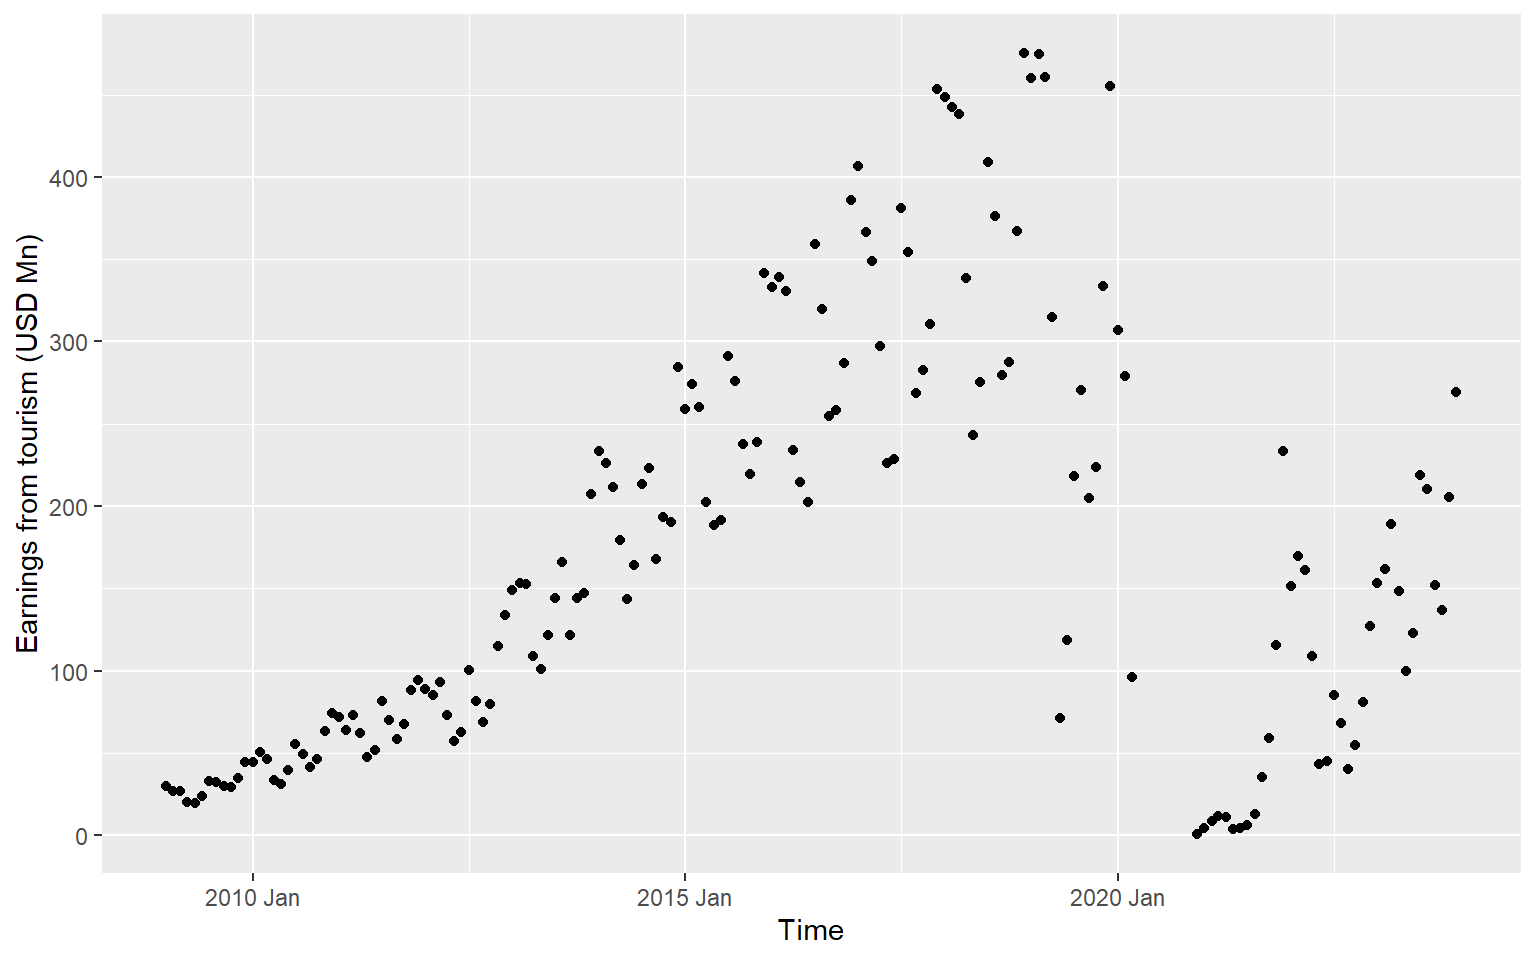
\includegraphics[keepaspectratio]{02-chap2_files/figure-pdf/unnamed-chunk-13-1.pdf}}

\begin{Shaded}
\begin{Highlighting}[]
\NormalTok{ts.earnings }\OtherTok{\textless{}{-}}\NormalTok{ y.earnings }\SpecialCharTok{|\textgreater{}}
  \FunctionTok{select}\NormalTok{(Earnings, Time) }\SpecialCharTok{|\textgreater{}} \FunctionTok{as\_tsibble}\NormalTok{(}\AttributeTok{index=}\NormalTok{Time)}
\NormalTok{ts.earnings}
\end{Highlighting}
\end{Shaded}

\begin{verbatim}
# A tsibble: 180 x 2 [1M]
   Earnings     Time
      <dbl>    <mth>
 1     30   2009 Jan
 2     26.7 2009 Feb
 3     26.6 2009 Mar
 4     20.3 2009 Apr
 5     19.3 2009 May
 6     23.6 2009 Jun
 7     33   2009 Jul
 8     32.2 2009 Aug
 9     29.6 2009 Sep
10     29.3 2009 Oct
# i 170 more rows
\end{verbatim}

\section{Time series visualisation using grammar of graphics:
R}\label{time-series-visualisation-using-grammar-of-graphics-r}

The grammar of graphics is a way of thinking about plots as layers. Each
plot is built from components like:

\textbf{Data} -- the dataset you are plotting.

\textbf{Aesthetics (aes)} -- how variables map to visual properties like
x, y, color, or size.

\textbf{Geometries (geom)} -- the type of plot (points, lines, bars,
etc.).

\textbf{Facets} -- split the plot into subplots based on a variable.

\textbf{Statistics (stat)} -- summary computations like regression lines
or counts.

\textbf{Scales} -- control axis limits, colors, or sizes.

\textbf{Coordinates (coord)} -- control coordinate system (Cartesian,
polar).

\textbf{Theme} -- control visual appearance like text, background, and
grid.

\begin{Shaded}
\begin{Highlighting}[]
\NormalTok{ggts }\OtherTok{\textless{}{-}}\NormalTok{ ts.earnings }\SpecialCharTok{|\textgreater{}}
  \FunctionTok{ggplot}\NormalTok{(}\FunctionTok{aes}\NormalTok{(}\AttributeTok{x =}\NormalTok{ Time, }\AttributeTok{y =}\NormalTok{ Earnings)) }\SpecialCharTok{+}
  \FunctionTok{geom\_point}\NormalTok{() }\SpecialCharTok{+}
  \FunctionTok{labs}\NormalTok{(}\AttributeTok{y =} \StringTok{"Earnings from tourism (USD Mn)"}\NormalTok{, }\AttributeTok{x=}\StringTok{"Time"}\NormalTok{)  }
\NormalTok{ggts}
\end{Highlighting}
\end{Shaded}

\pandocbounded{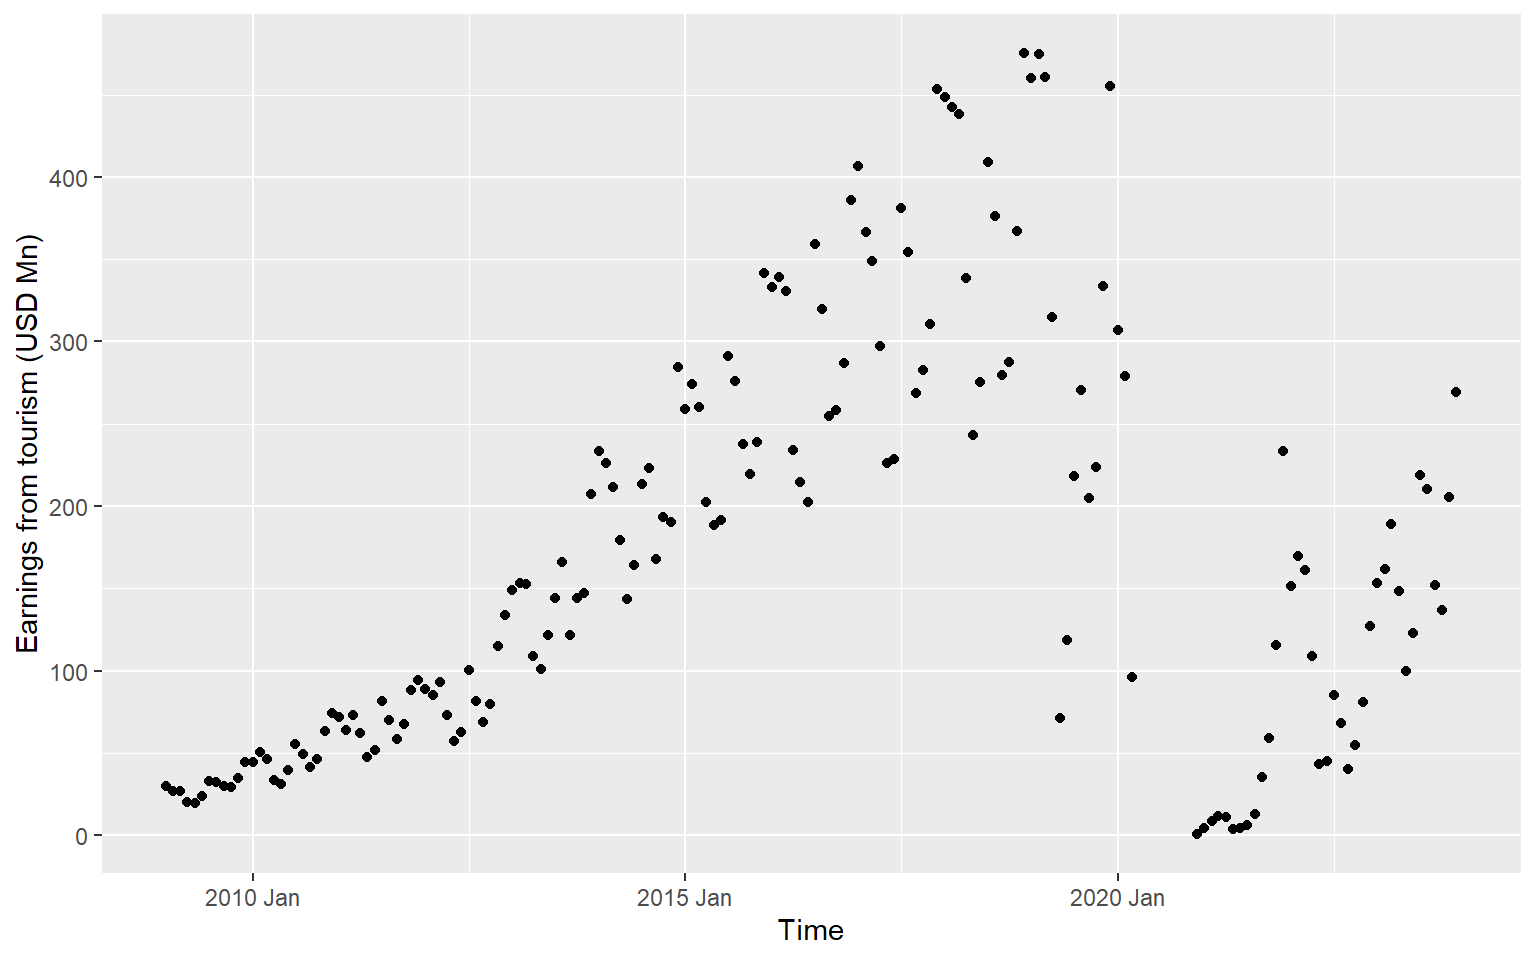
\includegraphics[keepaspectratio]{02-chap2_files/figure-pdf/unnamed-chunk-15-1.pdf}}

\begin{Shaded}
\begin{Highlighting}[]
\NormalTok{ggts }\OtherTok{\textless{}{-}}\NormalTok{ ts.earnings }\SpecialCharTok{|\textgreater{}}
  \FunctionTok{ggplot}\NormalTok{(}\FunctionTok{aes}\NormalTok{(}\AttributeTok{x =}\NormalTok{ Time, }\AttributeTok{y =}\NormalTok{ Earnings)) }\SpecialCharTok{+}
  \FunctionTok{geom\_line}\NormalTok{() }\SpecialCharTok{+}
  \FunctionTok{labs}\NormalTok{(}\AttributeTok{y =} \StringTok{"Earnings from tourism (USD Mn)"}\NormalTok{, }\AttributeTok{x=}\StringTok{"Time"}\NormalTok{)  }
\NormalTok{ggts}
\end{Highlighting}
\end{Shaded}

\pandocbounded{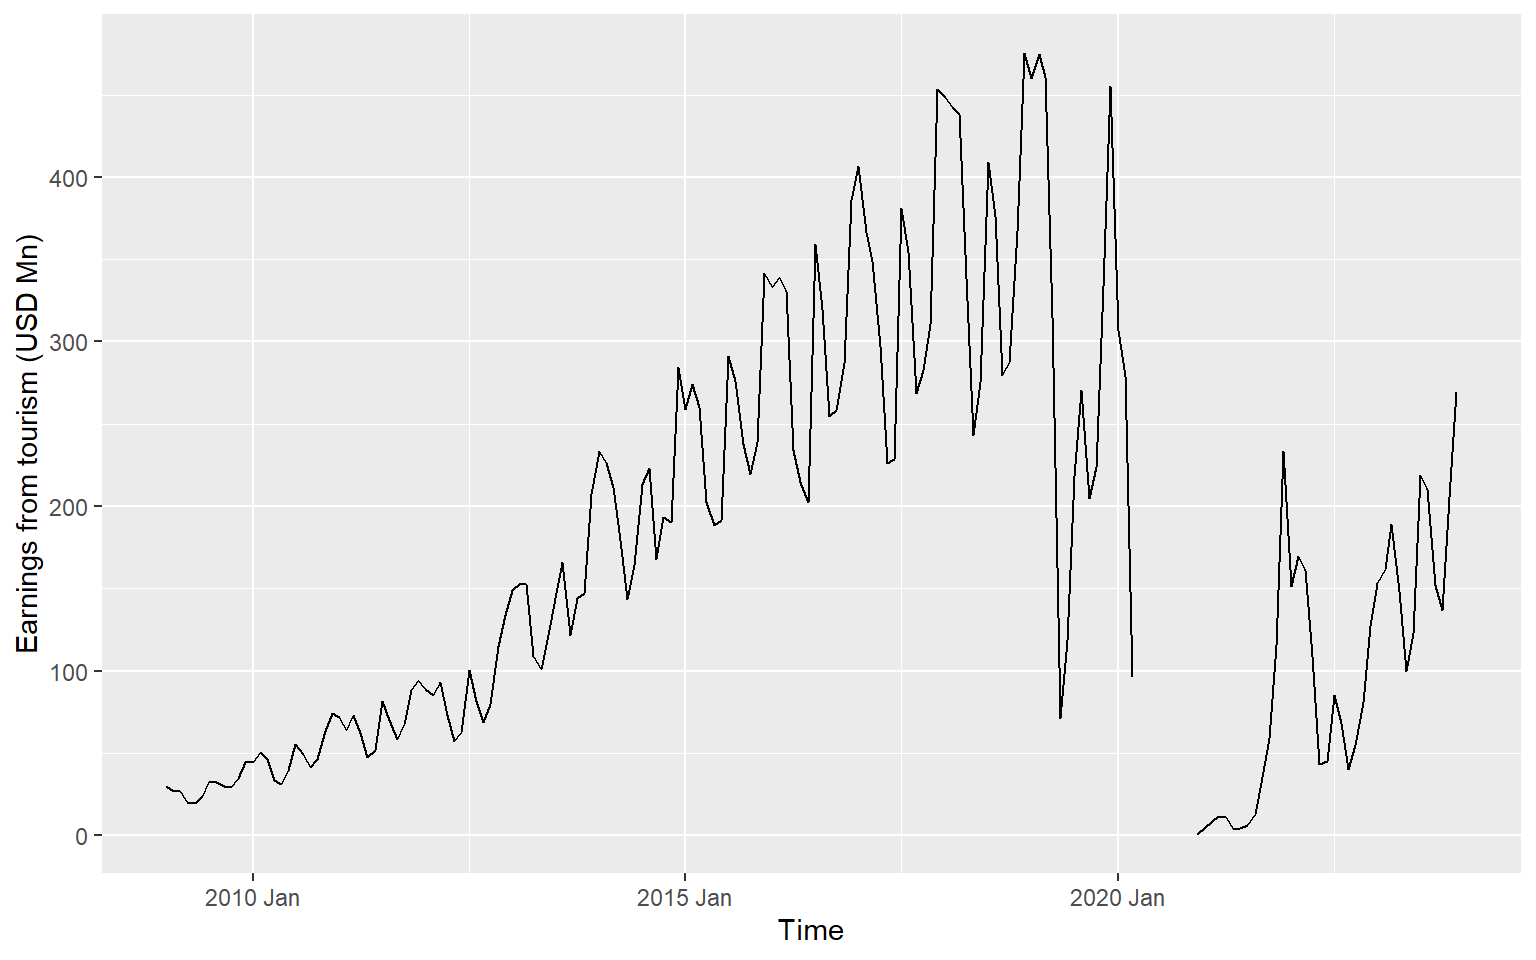
\includegraphics[keepaspectratio]{02-chap2_files/figure-pdf/unnamed-chunk-16-1.pdf}}

\begin{Shaded}
\begin{Highlighting}[]
\NormalTok{ts.earnings }\SpecialCharTok{|\textgreater{}}
    \FunctionTok{mutate}\NormalTok{(}\AttributeTok{Time =} \FunctionTok{as\_date}\NormalTok{(}\FunctionTok{yearmonth}\NormalTok{(Time))) }\SpecialCharTok{|\textgreater{}}
  \FunctionTok{ggplot}\NormalTok{(}\FunctionTok{aes}\NormalTok{(}\AttributeTok{x =}\NormalTok{ Time, }\AttributeTok{y =}\NormalTok{ Earnings)) }\SpecialCharTok{+}
  \FunctionTok{geom\_line}\NormalTok{() }\SpecialCharTok{+}
  \FunctionTok{scale\_x\_date}\NormalTok{(}\AttributeTok{date\_breaks =} \StringTok{"1 year"}\NormalTok{, }\AttributeTok{date\_labels =} \StringTok{"\%Y"}\NormalTok{) }\SpecialCharTok{+} 
  \FunctionTok{labs}\NormalTok{(}\AttributeTok{y =} \StringTok{"Earnings from tourism (USD Mn)"}\NormalTok{, }\AttributeTok{x=}\StringTok{"Time"}\NormalTok{) }
\end{Highlighting}
\end{Shaded}

\pandocbounded{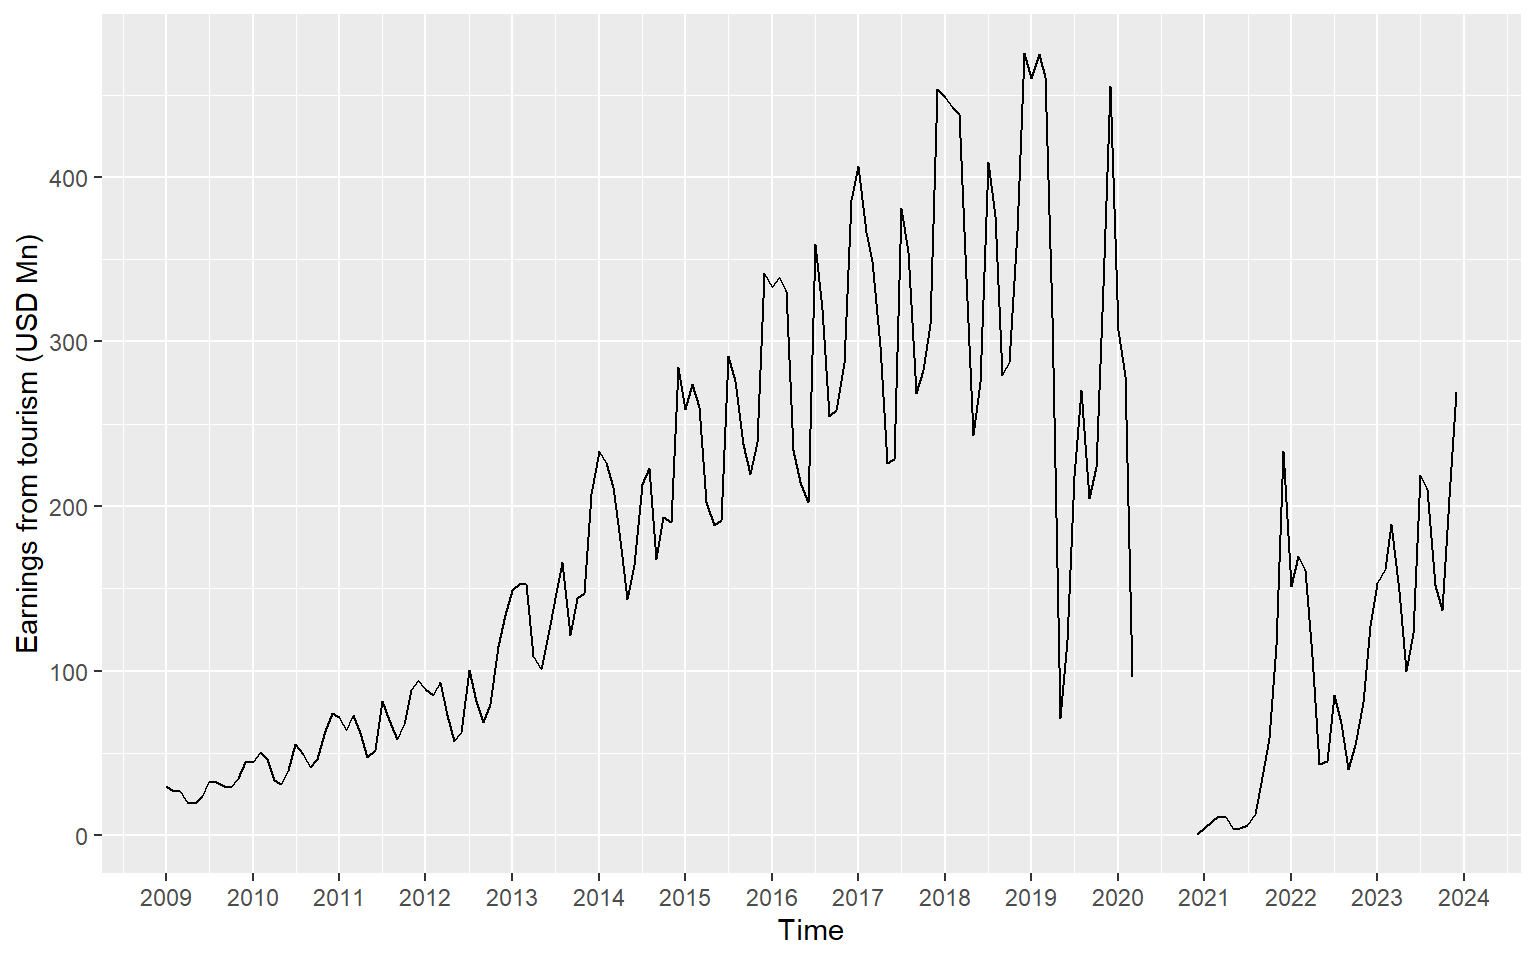
\includegraphics[keepaspectratio]{02-chap2_files/figure-pdf/unnamed-chunk-17-1.pdf}}

\begin{Shaded}
\begin{Highlighting}[]
\FunctionTok{library}\NormalTok{(viridis)}
\NormalTok{ts.earnings }\SpecialCharTok{|\textgreater{}}
  \FunctionTok{gg\_season}\NormalTok{(Earnings, }\AttributeTok{period =} \StringTok{"1 year"}\NormalTok{,  }\AttributeTok{pal =}\NormalTok{ scales}\SpecialCharTok{::}\FunctionTok{viridis\_pal}\NormalTok{()(}\DecValTok{15}\NormalTok{))  }\SpecialCharTok{+} \FunctionTok{geom\_point}\NormalTok{()  }
\end{Highlighting}
\end{Shaded}

\pandocbounded{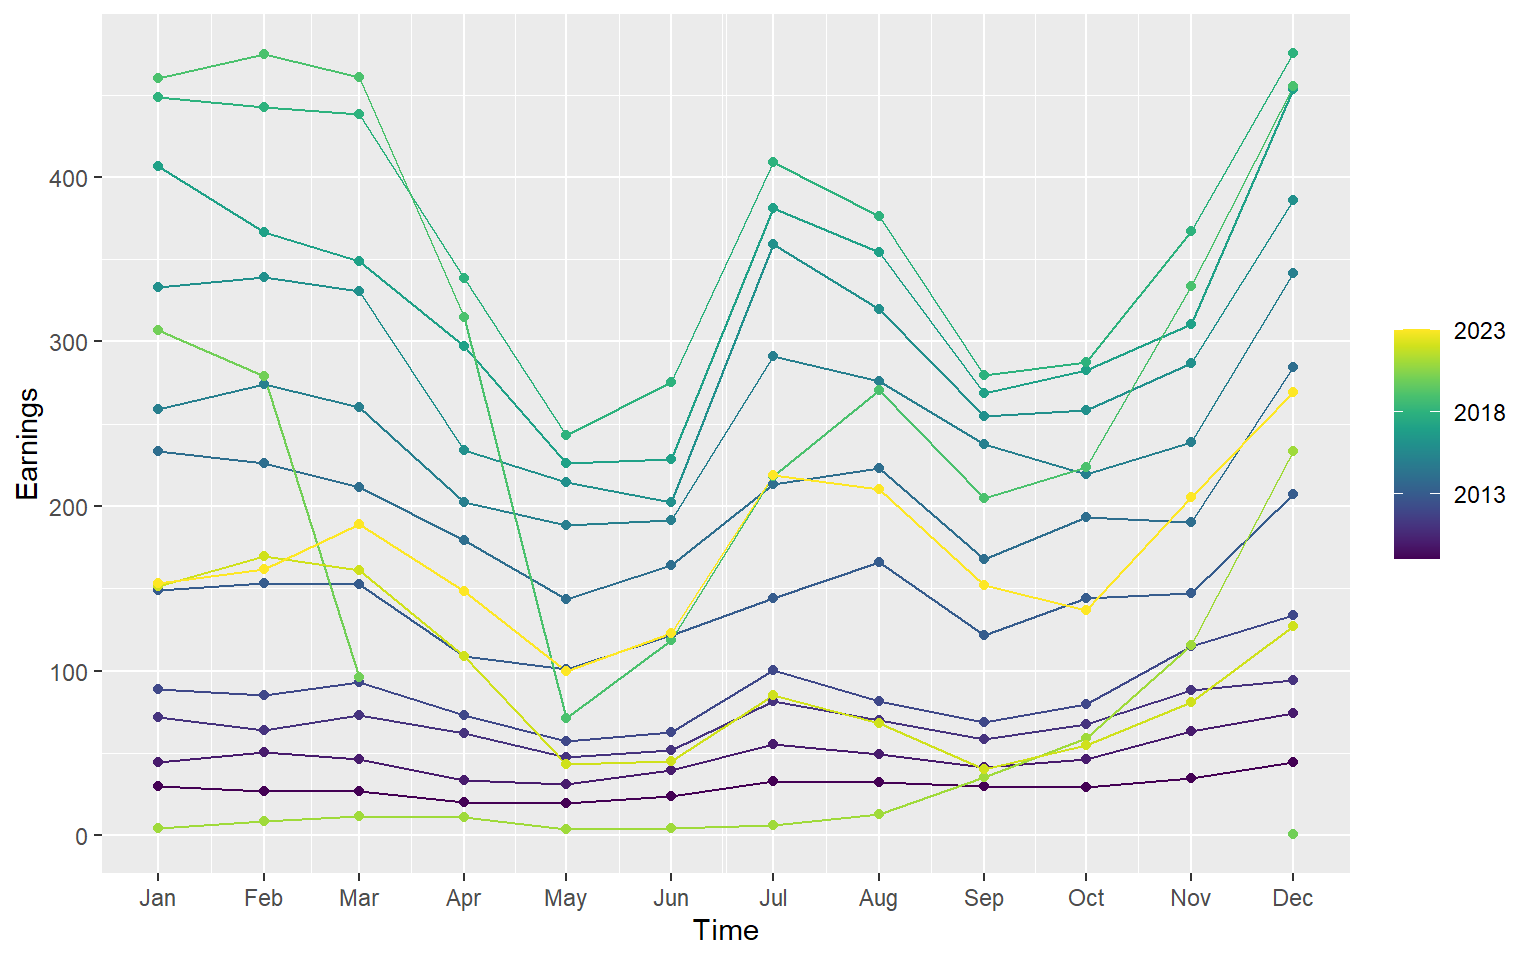
\includegraphics[keepaspectratio]{02-chap2_files/figure-pdf/unnamed-chunk-18-1.pdf}}

\section{Dataset: Python}\label{dataset-python}

\begin{Shaded}
\begin{Highlighting}[]
\ImportTok{import}\NormalTok{ plotnine }\ImportTok{as}\NormalTok{ p9}
\ImportTok{from}\NormalTok{ plotnine.data }\ImportTok{import}\NormalTok{ economics}
\end{Highlighting}
\end{Shaded}

\section{Working with Built-in Data
Set}\label{working-with-built-in-data-set}

\begin{Shaded}
\begin{Highlighting}[]
\ImportTok{import}\NormalTok{ pandas }\ImportTok{as}\NormalTok{ pd}
\ImportTok{import}\NormalTok{ plotnine }\ImportTok{as}\NormalTok{ p9 }
\ImportTok{from}\NormalTok{ plotnine }\ImportTok{import} \OperatorTok{*}
\ImportTok{from}\NormalTok{ plotnine.data }\ImportTok{import} \OperatorTok{*}
\ImportTok{import}\NormalTok{ numpy }\ImportTok{as}\NormalTok{ np}
\NormalTok{economics}
\end{Highlighting}
\end{Shaded}

\begin{verbatim}
          date      pce     pop  psavert  uempmed  unemploy
0   1967-07-01    507.4  198712     12.5      4.5      2944
1   1967-08-01    510.5  198911     12.5      4.7      2945
2   1967-09-01    516.3  199113     11.7      4.6      2958
3   1967-10-01    512.9  199311     12.5      4.9      3143
4   1967-11-01    518.1  199498     12.5      4.7      3066
..         ...      ...     ...      ...      ...       ...
569 2014-12-01  12122.0  320201      5.0     12.6      8688
570 2015-01-01  12080.8  320367      5.5     13.4      8979
571 2015-02-01  12095.9  320534      5.7     13.1      8705
572 2015-03-01  12161.5  320707      5.2     12.2      8575
573 2015-04-01  12158.9  320887      5.6     11.7      8549

[574 rows x 6 columns]
\end{verbatim}

\begin{Shaded}
\begin{Highlighting}[]
\NormalTok{economics.info()}
\end{Highlighting}
\end{Shaded}

\begin{verbatim}
<class 'pandas.core.frame.DataFrame'>
RangeIndex: 574 entries, 0 to 573
Data columns (total 6 columns):
 #   Column    Non-Null Count  Dtype         
---  ------    --------------  -----         
 0   date      574 non-null    datetime64[ns]
 1   pce       574 non-null    float64       
 2   pop       574 non-null    int64         
 3   psavert   574 non-null    float64       
 4   uempmed   574 non-null    float64       
 5   unemploy  574 non-null    int64         
dtypes: datetime64[ns](1), float64(3), int64(2)
memory usage: 27.0 KB
\end{verbatim}

\subsection{\texorpdfstring{Create \texttt{year} and \texttt{month}
columns}{Create year and month columns}}\label{create-year-and-month-columns}

\begin{Shaded}
\begin{Highlighting}[]
\NormalTok{economics[}\StringTok{\textquotesingle{}year\textquotesingle{}}\NormalTok{] }\OperatorTok{=}\NormalTok{ economics[}\StringTok{\textquotesingle{}date\textquotesingle{}}\NormalTok{].dt.year}
\NormalTok{economics[}\StringTok{\textquotesingle{}month\textquotesingle{}}\NormalTok{] }\OperatorTok{=}\NormalTok{ economics[}\StringTok{\textquotesingle{}date\textquotesingle{}}\NormalTok{].dt.month}
\NormalTok{economics}
\end{Highlighting}
\end{Shaded}

\begin{verbatim}
          date      pce     pop  psavert  uempmed  unemploy  year  month
0   1967-07-01    507.4  198712     12.5      4.5      2944  1967      7
1   1967-08-01    510.5  198911     12.5      4.7      2945  1967      8
2   1967-09-01    516.3  199113     11.7      4.6      2958  1967      9
3   1967-10-01    512.9  199311     12.5      4.9      3143  1967     10
4   1967-11-01    518.1  199498     12.5      4.7      3066  1967     11
..         ...      ...     ...      ...      ...       ...   ...    ...
569 2014-12-01  12122.0  320201      5.0     12.6      8688  2014     12
570 2015-01-01  12080.8  320367      5.5     13.4      8979  2015      1
571 2015-02-01  12095.9  320534      5.7     13.1      8705  2015      2
572 2015-03-01  12161.5  320707      5.2     12.2      8575  2015      3
573 2015-04-01  12158.9  320887      5.6     11.7      8549  2015      4

[574 rows x 8 columns]
\end{verbatim}

\section{Time series visualisation using grammar of graphics:
Python}\label{time-series-visualisation-using-grammar-of-graphics-python}

The grammar of graphics is a way of thinking about plots as layers. Each
plot is built from components like:

\textbf{Data} -- the dataset you are plotting.

\textbf{Aesthetics (aes)} -- how variables map to visual properties like
x, y, color, or size.

\textbf{Geometries (geom)} -- the type of plot (points, lines, bars,
etc.).

\textbf{Facets} -- split the plot into subplots based on a variable.

\textbf{Statistics (stat)} -- summary computations like regression lines
or counts.

\textbf{Scales} -- control axis limits, colors, or sizes.

\textbf{Coordinates (coord)} -- control coordinate system (Cartesian,
polar).

\textbf{Theme} -- control visual appearance like text, background, and
grid.

\href{https://thiyangt.github.io/spts_python_practical/Practical1/}{*}

\section{What is a lag value?}\label{what-is-a-lag-value}

In time series analysis, a lag represents the number of time steps by
which a series is shifted backward to compare it with itself.

Lag 1: Compare each value with the previous observation.

Lag 2: Compare each value with the value two steps before.

Lag k: Compare each value with the value k steps earlier.

\begin{Shaded}
\begin{Highlighting}[]
\ImportTok{import}\NormalTok{ pandas }\ImportTok{as}\NormalTok{ pd}

\CommentTok{\# Small time series with 5 points}
\NormalTok{data }\OperatorTok{=}\NormalTok{ [}\DecValTok{10}\NormalTok{, }\DecValTok{12}\NormalTok{, }\DecValTok{13}\NormalTok{, }\DecValTok{15}\NormalTok{, }\DecValTok{14}\NormalTok{]}
\NormalTok{dates }\OperatorTok{=}\NormalTok{ pd.date\_range(start}\OperatorTok{=}\StringTok{\textquotesingle{}2025{-}01{-}01\textquotesingle{}}\NormalTok{, periods}\OperatorTok{=}\DecValTok{5}\NormalTok{, freq}\OperatorTok{=}\StringTok{\textquotesingle{}D\textquotesingle{}}\NormalTok{)}

\NormalTok{df }\OperatorTok{=}\NormalTok{ pd.DataFrame(\{}\StringTok{\textquotesingle{}Date\textquotesingle{}}\NormalTok{: dates, }\StringTok{\textquotesingle{}Value\textquotesingle{}}\NormalTok{: data\})}
\NormalTok{df.set\_index(}\StringTok{\textquotesingle{}Date\textquotesingle{}}\NormalTok{, inplace}\OperatorTok{=}\VariableTok{True}\NormalTok{)}

\CommentTok{\# Create lagged series}
\NormalTok{df[}\StringTok{\textquotesingle{}Lag1\textquotesingle{}}\NormalTok{] }\OperatorTok{=}\NormalTok{ df[}\StringTok{\textquotesingle{}Value\textquotesingle{}}\NormalTok{].shift(}\DecValTok{1}\NormalTok{)  }\CommentTok{\# lag 1}
\NormalTok{df[}\StringTok{\textquotesingle{}Lag2\textquotesingle{}}\NormalTok{] }\OperatorTok{=}\NormalTok{ df[}\StringTok{\textquotesingle{}Value\textquotesingle{}}\NormalTok{].shift(}\DecValTok{2}\NormalTok{)  }\CommentTok{\# lag 2}

\CommentTok{\# Show the result}
\BuiltInTok{print}\NormalTok{(df)}
\end{Highlighting}
\end{Shaded}

\begin{verbatim}
            Value  Lag1  Lag2
Date                         
2025-01-01     10   NaN   NaN
2025-01-02     12  10.0   NaN
2025-01-03     13  12.0  10.0
2025-01-04     15  13.0  12.0
2025-01-05     14  15.0  13.0
\end{verbatim}

\section{Correlation vs
Autocorrelation}\label{correlation-vs-autocorrelation}

\subsection{Correlation}\label{correlation}

Measures the strength of the linear relationship between two variables

\[r = \frac{\sum_{i=1}^{n} (x_i -\bar{x})(y_i-\bar{y})}{\sqrt{\sum_{i=1}^{n} (x_i -\bar{x})^2 \sum_{i=1}^{n} (y_i -\bar{y})^2}}\]

\subsection{Autocorrelation}\label{autocorrelation}

Measures the strength of linear relationship between lagged values of
time series.

\[r_k = \frac{\sum (y_t -\bar{y})(y_{t-k}-\bar{y})}{\sum (y_t -\bar{y})^2}\]

\section{Your turn: why different
values?}\label{your-turn-why-different-values}

\begin{Shaded}
\begin{Highlighting}[]
\CommentTok{\# Correlation (autocorrelation) between original series and lagged series}
\NormalTok{autocorr\_lag1 }\OperatorTok{=}\NormalTok{ df[}\StringTok{\textquotesingle{}Value\textquotesingle{}}\NormalTok{].corr(df[}\StringTok{\textquotesingle{}Lag1\textquotesingle{}}\NormalTok{])}
\NormalTok{autocorr\_lag2 }\OperatorTok{=}\NormalTok{ df[}\StringTok{\textquotesingle{}Value\textquotesingle{}}\NormalTok{].corr(df[}\StringTok{\textquotesingle{}Lag2\textquotesingle{}}\NormalTok{])}

\BuiltInTok{print}\NormalTok{(}\SpecialStringTok{f"Autocorrelation at lag 1: }\SpecialCharTok{\{}\NormalTok{autocorr\_lag1}\SpecialCharTok{:.3f\}}\SpecialStringTok{"}\NormalTok{)}
\end{Highlighting}
\end{Shaded}

\begin{verbatim}
Autocorrelation at lag 1: 0.744
\end{verbatim}

\begin{Shaded}
\begin{Highlighting}[]
\BuiltInTok{print}\NormalTok{(}\SpecialStringTok{f"Autocorrelation at lag 2: }\SpecialCharTok{\{}\NormalTok{autocorr\_lag2}\SpecialCharTok{:.3f\}}\SpecialStringTok{"}\NormalTok{)}
\end{Highlighting}
\end{Shaded}

\begin{verbatim}
Autocorrelation at lag 2: 0.655
\end{verbatim}

\begin{Shaded}
\begin{Highlighting}[]
\ImportTok{import}\NormalTok{ pandas }\ImportTok{as}\NormalTok{ pd}
\ImportTok{import}\NormalTok{ numpy }\ImportTok{as}\NormalTok{ np}
\ImportTok{import}\NormalTok{ matplotlib.pyplot }\ImportTok{as}\NormalTok{ plt}
\ImportTok{from}\NormalTok{ statsmodels.tsa.stattools }\ImportTok{import}\NormalTok{ acf}

\CommentTok{\# Small time series with 5 points}
\NormalTok{data }\OperatorTok{=}\NormalTok{ [}\DecValTok{10}\NormalTok{, }\DecValTok{12}\NormalTok{, }\DecValTok{13}\NormalTok{, }\DecValTok{15}\NormalTok{, }\DecValTok{14}\NormalTok{]}
\NormalTok{dates }\OperatorTok{=}\NormalTok{ pd.date\_range(start}\OperatorTok{=}\StringTok{\textquotesingle{}2025{-}01{-}01\textquotesingle{}}\NormalTok{, periods}\OperatorTok{=}\DecValTok{5}\NormalTok{, freq}\OperatorTok{=}\StringTok{\textquotesingle{}D\textquotesingle{}}\NormalTok{)}

\NormalTok{df }\OperatorTok{=}\NormalTok{ pd.DataFrame(\{}\StringTok{\textquotesingle{}Date\textquotesingle{}}\NormalTok{: dates, }\StringTok{\textquotesingle{}Value\textquotesingle{}}\NormalTok{: data\})}
\NormalTok{df.set\_index(}\StringTok{\textquotesingle{}Date\textquotesingle{}}\NormalTok{, inplace}\OperatorTok{=}\VariableTok{True}\NormalTok{)}

\BuiltInTok{print}\NormalTok{(df)}
\end{Highlighting}
\end{Shaded}

\begin{verbatim}
            Value
Date             
2025-01-01     10
2025-01-02     12
2025-01-03     13
2025-01-04     15
2025-01-05     14
\end{verbatim}

\begin{Shaded}
\begin{Highlighting}[]
\CommentTok{\# Compute autocorrelation for lags 1 to 4 (max lag = n{-}1)}
\NormalTok{autocorr\_values }\OperatorTok{=}\NormalTok{ acf(df[}\StringTok{\textquotesingle{}Value\textquotesingle{}}\NormalTok{], nlags}\OperatorTok{=}\DecValTok{4}\NormalTok{, fft}\OperatorTok{=}\VariableTok{False}\NormalTok{)}

\CommentTok{\# Show autocorrelation values}
\ControlFlowTok{for}\NormalTok{ lag, val }\KeywordTok{in} \BuiltInTok{enumerate}\NormalTok{(autocorr\_values):}
    \BuiltInTok{print}\NormalTok{(}\SpecialStringTok{f"Lag }\SpecialCharTok{\{}\NormalTok{lag}\SpecialCharTok{\}}\SpecialStringTok{: }\SpecialCharTok{\{}\NormalTok{val}\SpecialCharTok{:.3f\}}\SpecialStringTok{"}\NormalTok{)}
\end{Highlighting}
\end{Shaded}

\begin{verbatim}
Lag 0: 1.000
Lag 1: 0.349
Lag 2: -0.141
Lag 3: -0.481
Lag 4: -0.227
\end{verbatim}

\section{Autocorrelation plots (ACF)}\label{autocorrelation-plots-acf}

The ACF measures the correlation between a time series and lagged
versions of itself. It tells us how past values influence current
values.

\subsection{Example 1}\label{example-1}

Time series plot

\begin{Shaded}
\begin{Highlighting}[]
\FunctionTok{library}\NormalTok{(fable)}
\FunctionTok{library}\NormalTok{(fpp2)}
\FunctionTok{autoplot}\NormalTok{(beer)}
\end{Highlighting}
\end{Shaded}

\pandocbounded{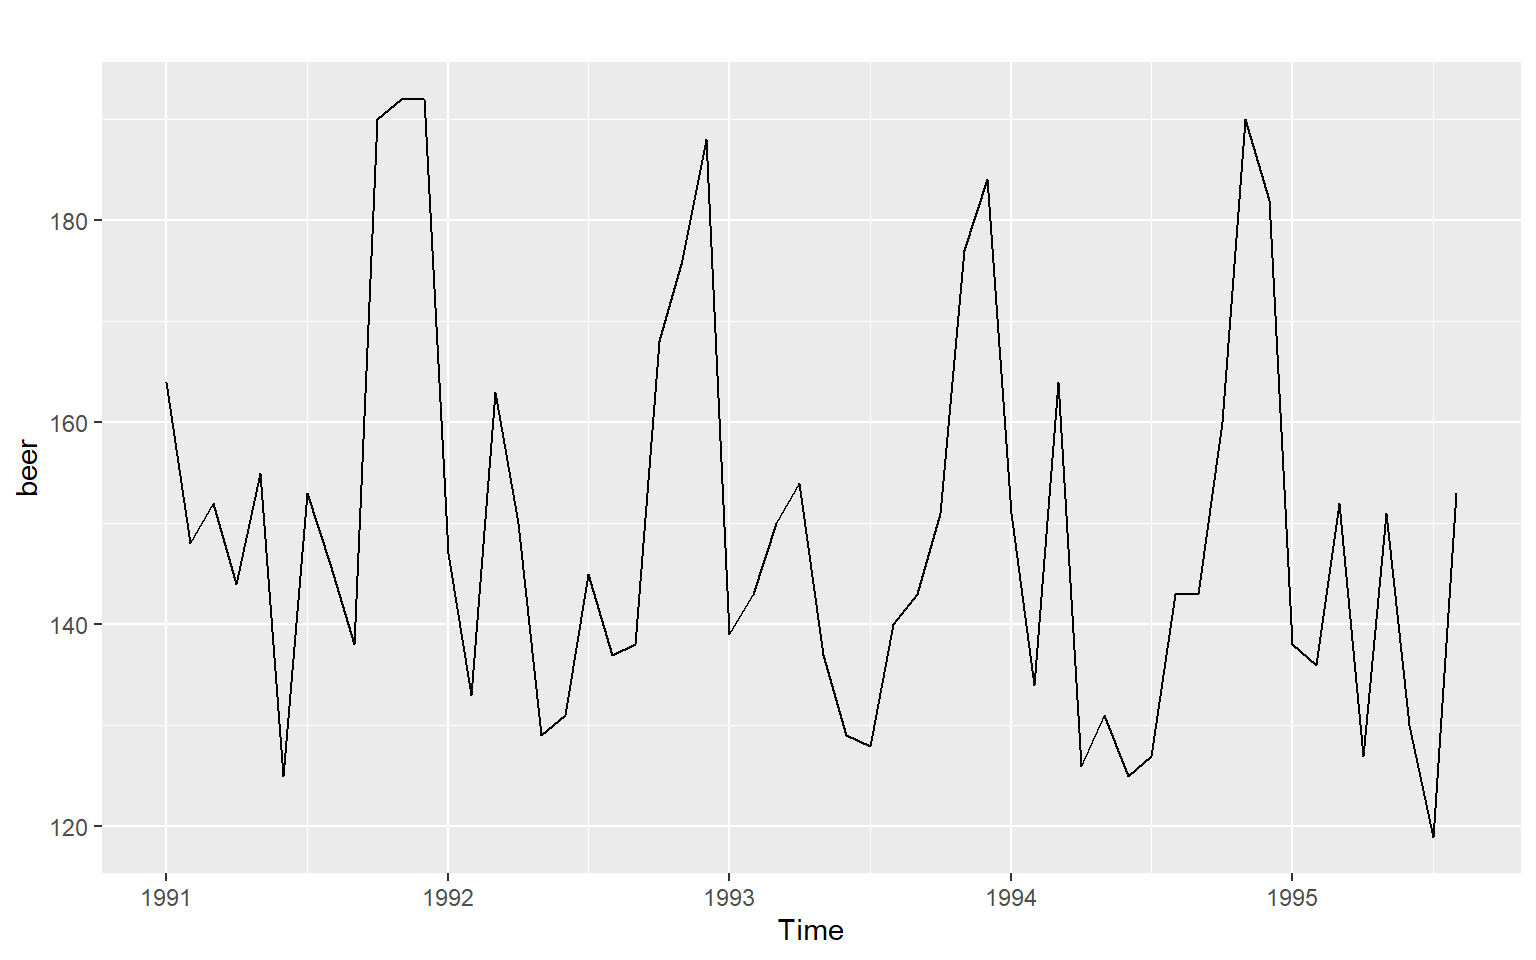
\includegraphics[keepaspectratio]{02-chap2_files/figure-pdf/unnamed-chunk-27-1.pdf}}

Seasonal plot

\begin{Shaded}
\begin{Highlighting}[]
\FunctionTok{ggseasonplot}\NormalTok{(beer, }\AttributeTok{year.labels=}\ConstantTok{TRUE}\NormalTok{, }\AttributeTok{year.labels.left=}\ConstantTok{TRUE}\NormalTok{)}
\end{Highlighting}
\end{Shaded}

\pandocbounded{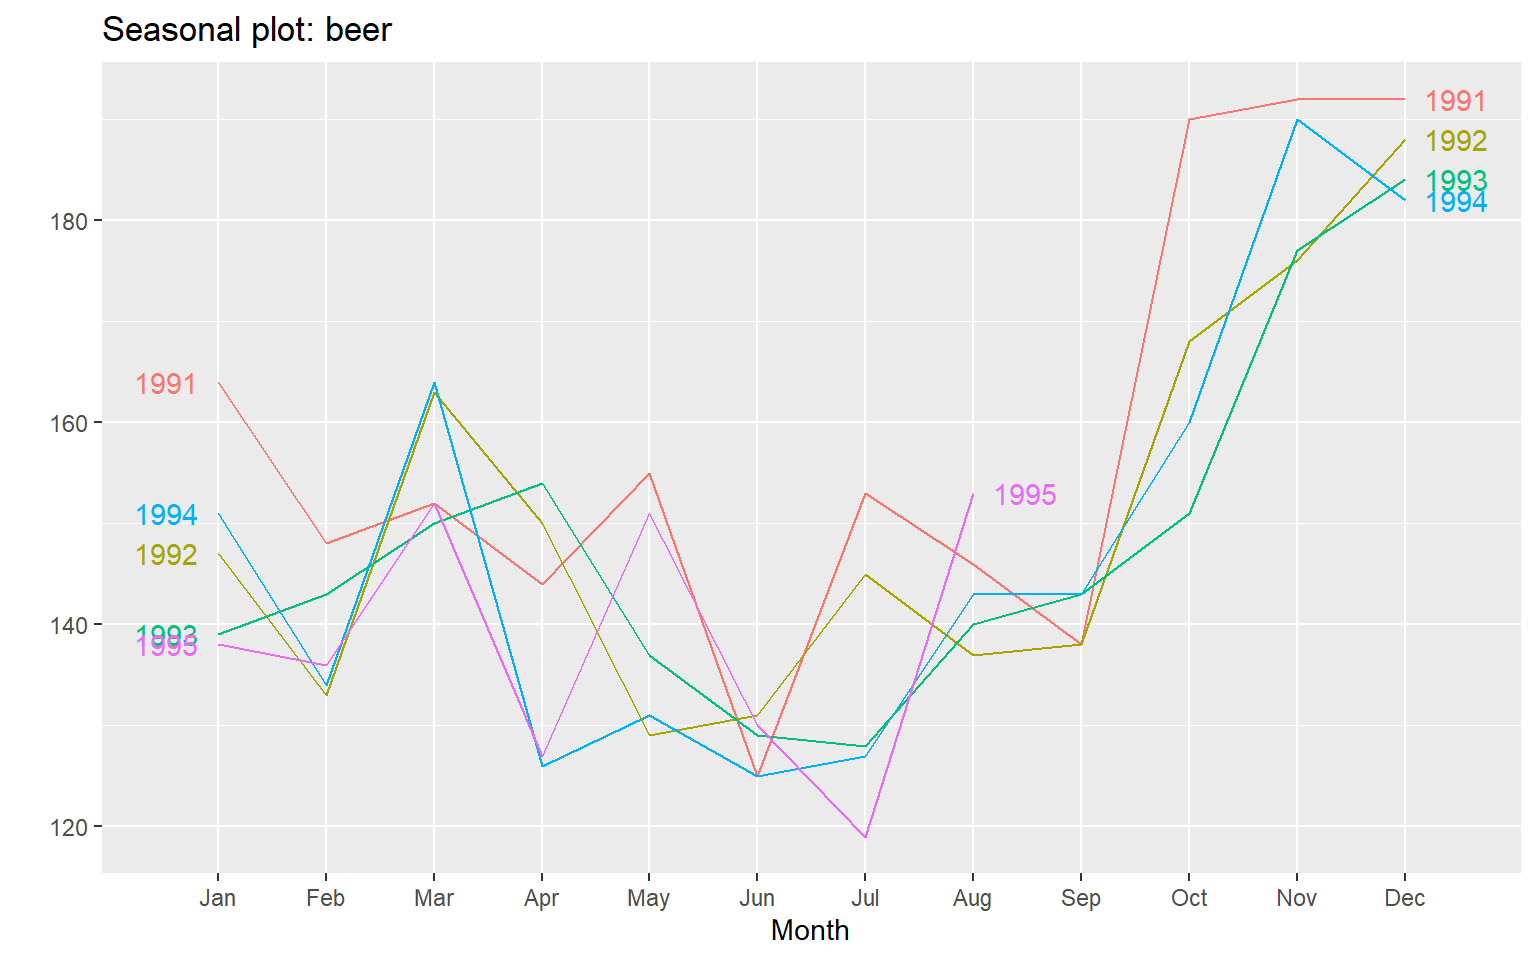
\includegraphics[keepaspectratio]{02-chap2_files/figure-pdf/unnamed-chunk-28-1.pdf}}

ACF

\begin{Shaded}
\begin{Highlighting}[]
\FunctionTok{ggAcf}\NormalTok{(beer)}
\end{Highlighting}
\end{Shaded}

\pandocbounded{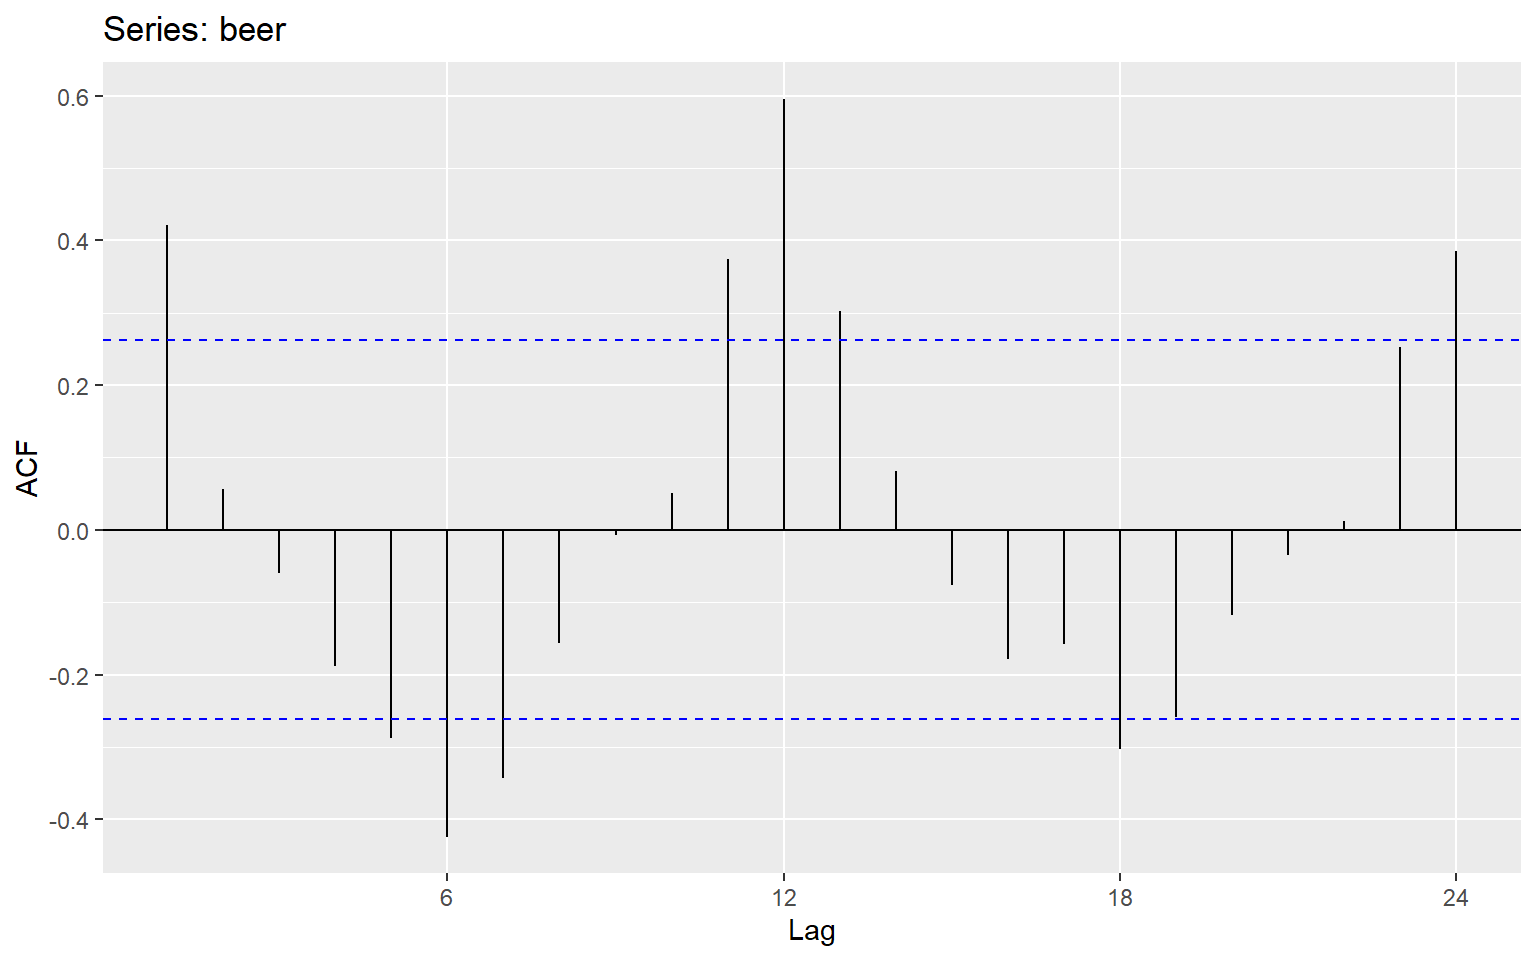
\includegraphics[keepaspectratio]{02-chap2_files/figure-pdf/unnamed-chunk-29-1.pdf}}

\begin{Shaded}
\begin{Highlighting}[]
\FunctionTok{ggseasonplot}\NormalTok{(beer, }\AttributeTok{year.labels=}\ConstantTok{TRUE}\NormalTok{, }\AttributeTok{year.labels.left=}\ConstantTok{TRUE}\NormalTok{)}
\end{Highlighting}
\end{Shaded}

\pandocbounded{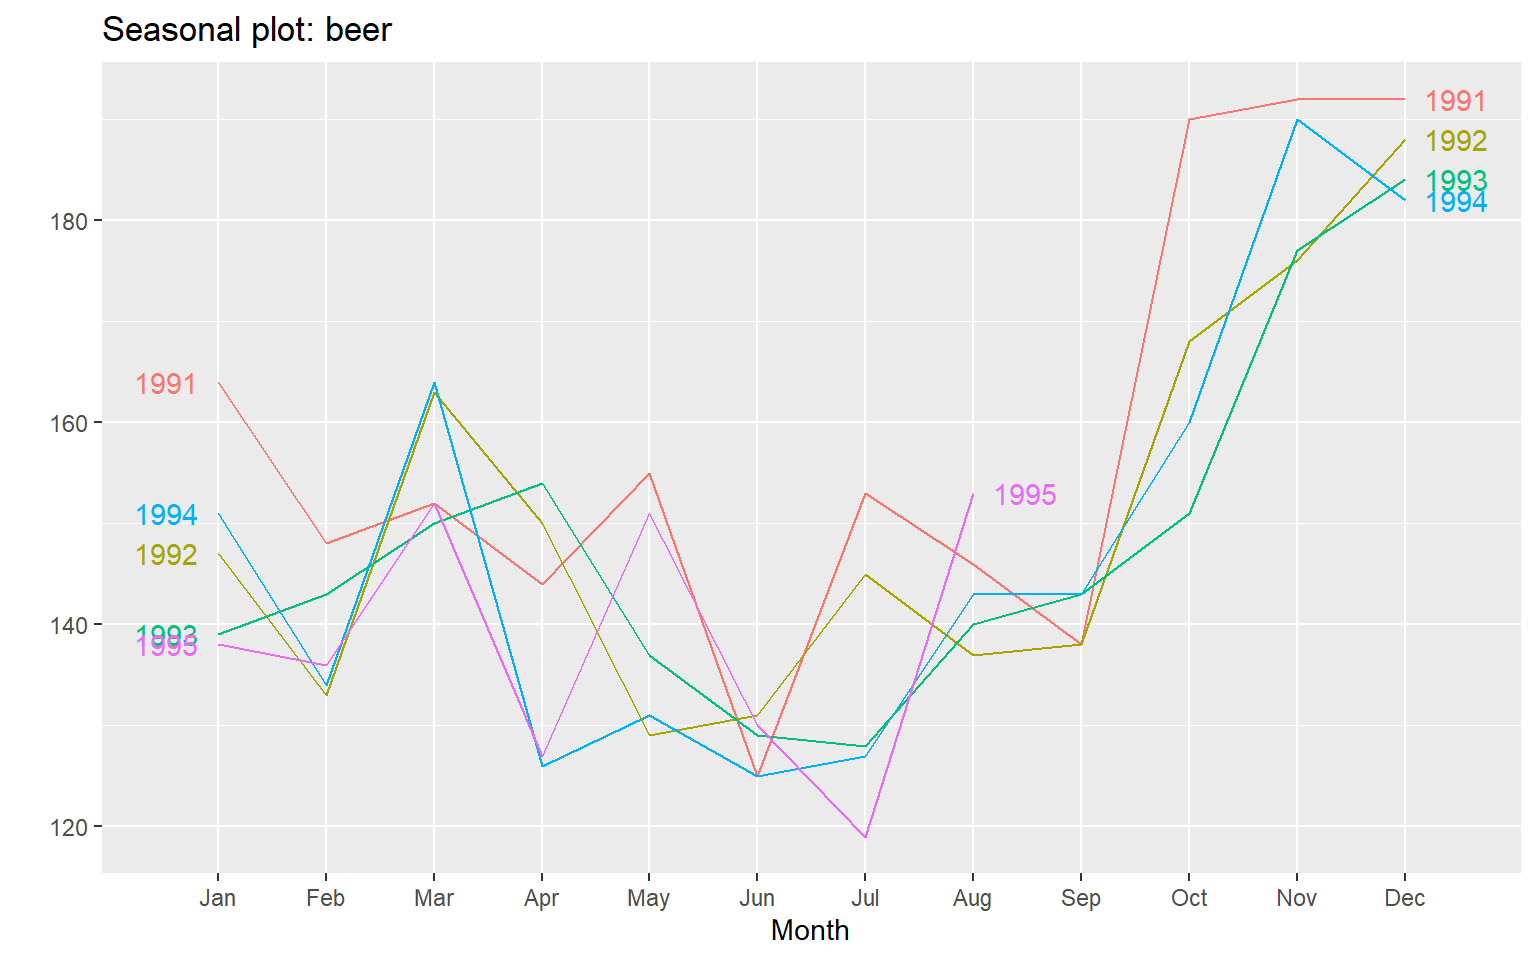
\includegraphics[keepaspectratio]{02-chap2_files/figure-pdf/unnamed-chunk-30-1.pdf}}

\section{Example 2}\label{example-2}

\begin{Shaded}
\begin{Highlighting}[]
\NormalTok{aelec }\OtherTok{\textless{}{-}} \FunctionTok{window}\NormalTok{(elec, }\AttributeTok{start=}\DecValTok{1980}\NormalTok{)}
\FunctionTok{autoplot}\NormalTok{(aelec) }\SpecialCharTok{+} \FunctionTok{xlab}\NormalTok{(}\StringTok{"Year"}\NormalTok{) }\SpecialCharTok{+} \FunctionTok{ylab}\NormalTok{(}\StringTok{"GWh"}\NormalTok{)}
\end{Highlighting}
\end{Shaded}

\pandocbounded{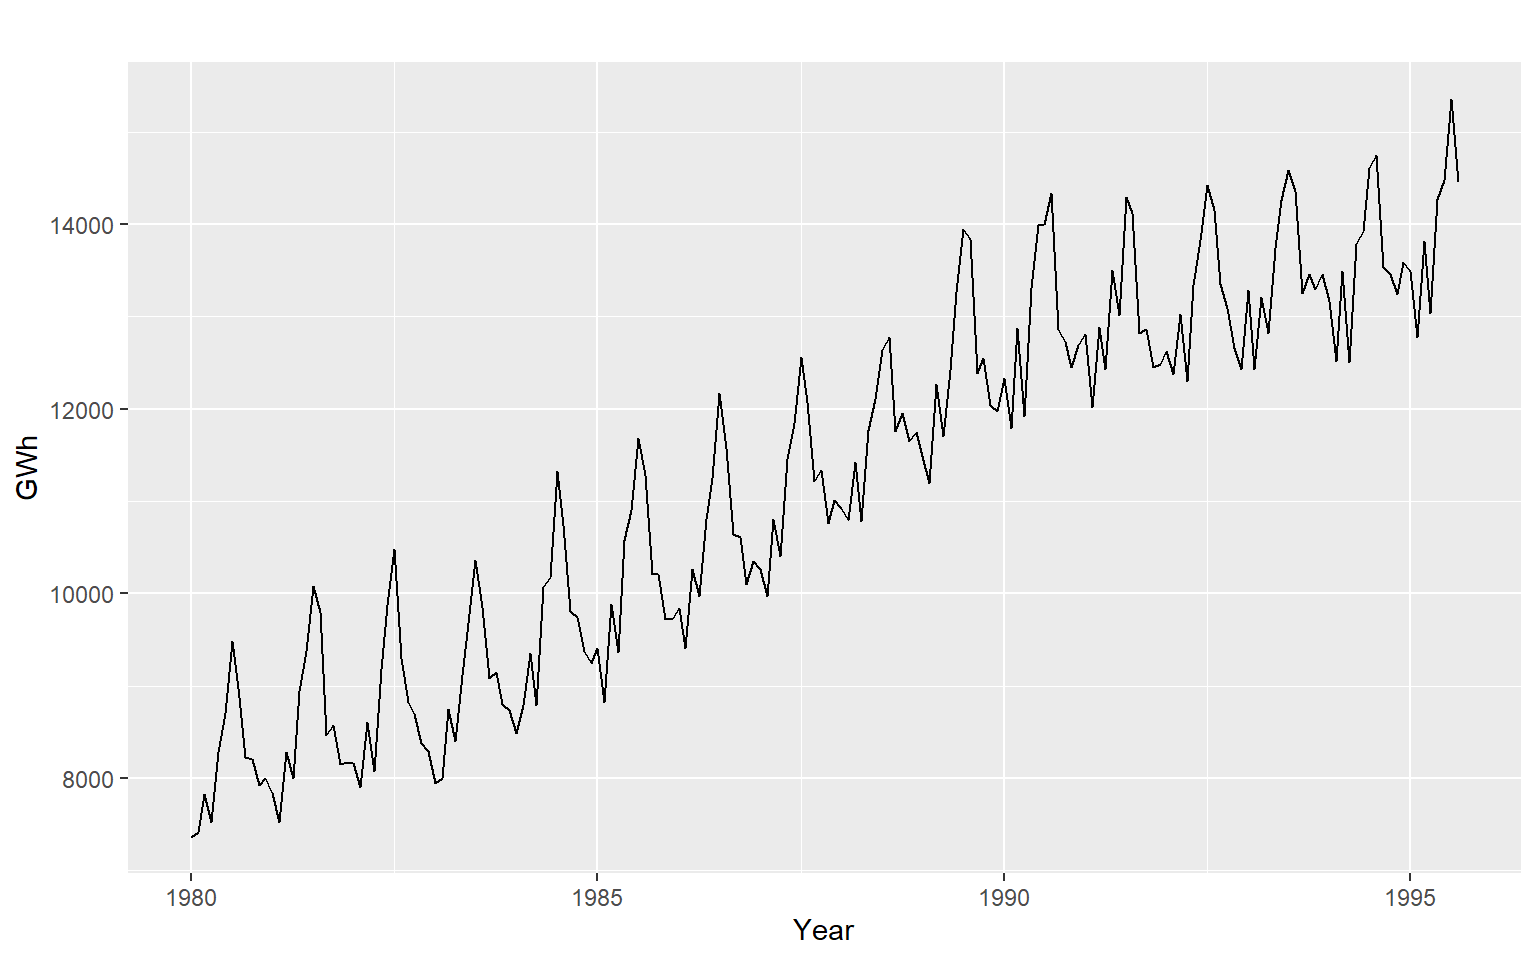
\includegraphics[keepaspectratio]{02-chap2_files/figure-pdf/unnamed-chunk-31-1.pdf}}

Seasonal plots

\begin{Shaded}
\begin{Highlighting}[]
\FunctionTok{ggseasonplot}\NormalTok{(aelec, }\AttributeTok{year.labels=}\ConstantTok{TRUE}\NormalTok{, }\AttributeTok{year.labels.left=}\ConstantTok{TRUE}\NormalTok{)}
\end{Highlighting}
\end{Shaded}

\pandocbounded{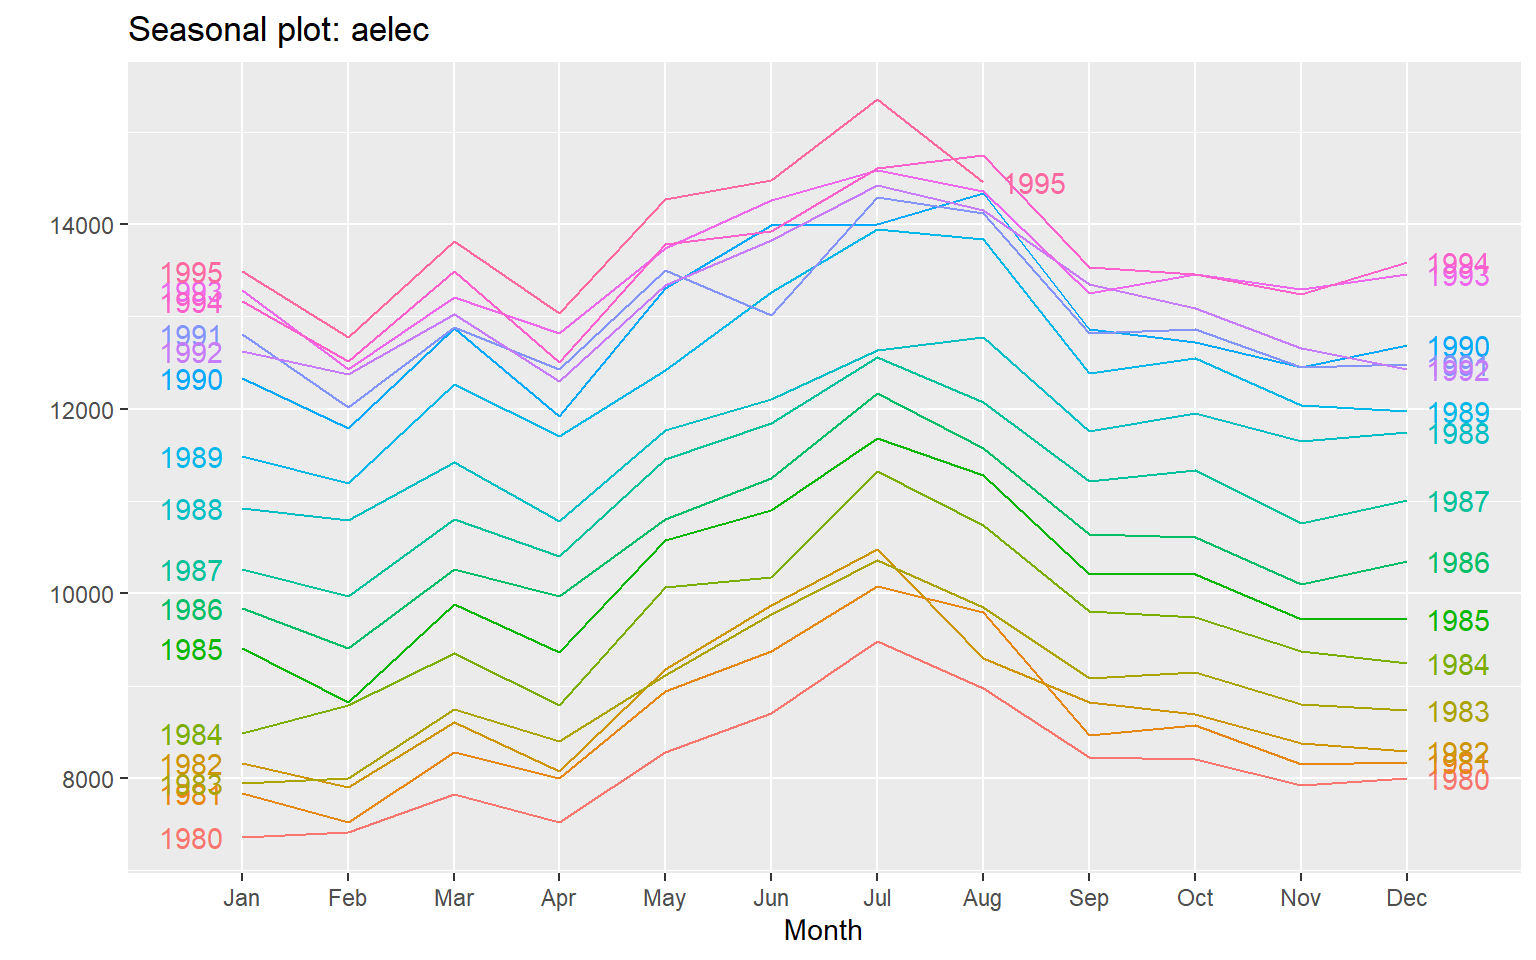
\includegraphics[keepaspectratio]{02-chap2_files/figure-pdf/unnamed-chunk-32-1.pdf}}

\begin{Shaded}
\begin{Highlighting}[]
\FunctionTok{ggAcf}\NormalTok{(aelec, }\AttributeTok{lag=}\DecValTok{48}\NormalTok{)}
\end{Highlighting}
\end{Shaded}

\pandocbounded{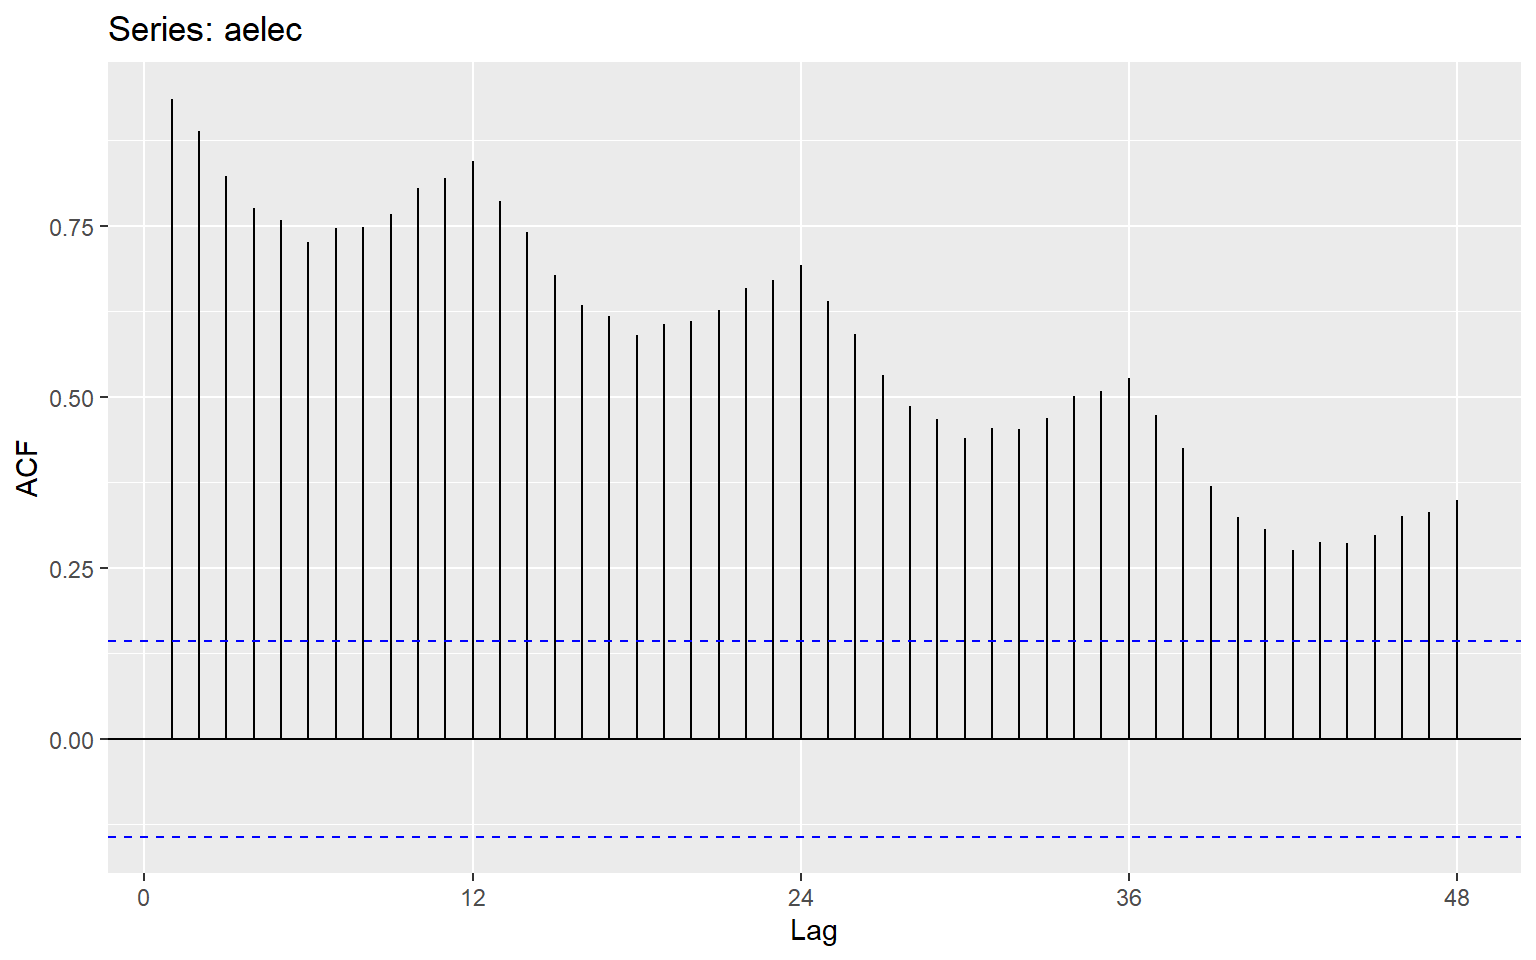
\includegraphics[keepaspectratio]{02-chap2_files/figure-pdf/unnamed-chunk-33-1.pdf}}

\section{Example 3}\label{example-3}

\begin{Shaded}
\begin{Highlighting}[]
\FunctionTok{set.seed}\NormalTok{(}\DecValTok{3}\NormalTok{)}
\NormalTok{y }\OtherTok{\textless{}{-}} \FunctionTok{ts}\NormalTok{(}\FunctionTok{rnorm}\NormalTok{(}\DecValTok{50}\NormalTok{))}
\FunctionTok{autoplot}\NormalTok{(y) }\SpecialCharTok{+} \FunctionTok{ggtitle}\NormalTok{(}\StringTok{"White noise"}\NormalTok{)}
\end{Highlighting}
\end{Shaded}

\pandocbounded{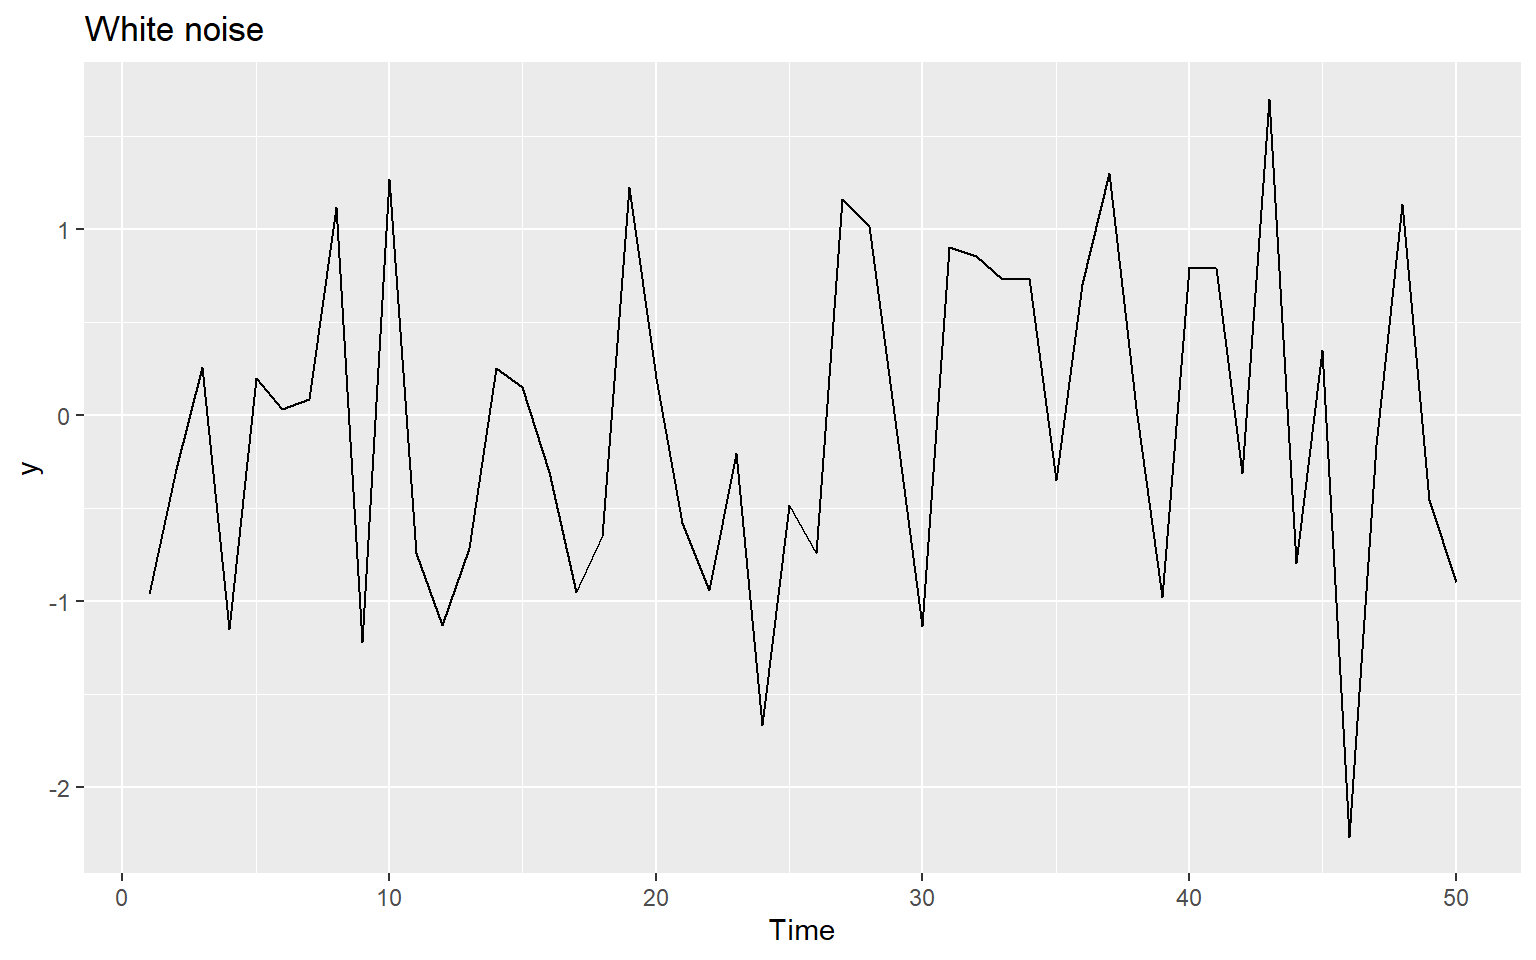
\includegraphics[keepaspectratio]{02-chap2_files/figure-pdf/unnamed-chunk-34-1.pdf}}

\begin{Shaded}
\begin{Highlighting}[]
\FunctionTok{ggAcf}\NormalTok{(y)}
\end{Highlighting}
\end{Shaded}

\pandocbounded{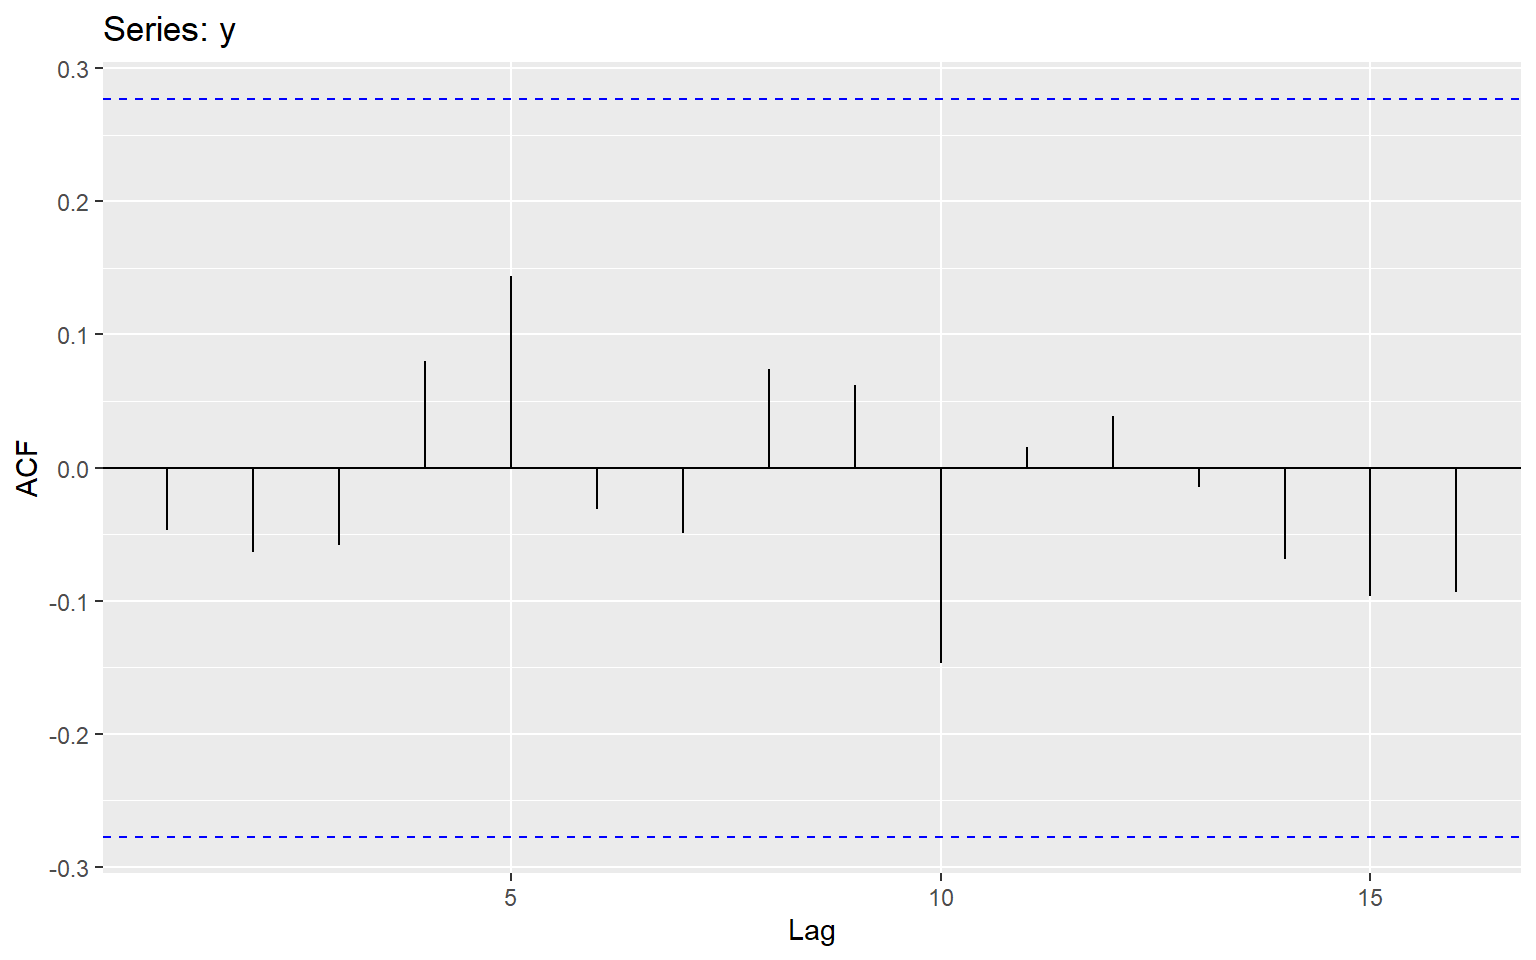
\includegraphics[keepaspectratio]{02-chap2_files/figure-pdf/unnamed-chunk-35-1.pdf}}

\section{Exercise}\label{exercise}

Question 6 at \url{https://otexts.com/fpp2/graphics-exercises.html}

\bookmarksetup{startatroot}

\chapter{Introduction to Time Series
Forecasting}\label{introduction-to-time-series-forecasting}

\section{Notation}\label{notation}

\(\hat{Y}_{T+h|T}\) - The forecast of the time series \(𝑌\) at time
\(T+h\), made using the information available up to time \(T\).

\section{Simple time series forecasting
techniques}\label{simple-time-series-forecasting-techniques}

\begin{enumerate}
\def\labelenumi{\arabic{enumi}.}
\item
  Average method
\item
  Naive method/ random walk method
\item
  Seasonal naive method
\item
  Drift method
\end{enumerate}

\href{https://otexts.com/fpp2/simple-methods.html}{Reading}

\section{Example: Electricity Demand
Forecasting}\label{example-electricity-demand-forecasting}

\begin{Shaded}
\begin{Highlighting}[]
\FunctionTok{library}\NormalTok{(fable)}
\FunctionTok{library}\NormalTok{(fpp2)}
\end{Highlighting}
\end{Shaded}

\begin{Shaded}
\begin{Highlighting}[]
\NormalTok{aelec }\OtherTok{\textless{}{-}} \FunctionTok{window}\NormalTok{(elec, }\AttributeTok{start=}\DecValTok{1980}\NormalTok{)}
\FunctionTok{autoplot}\NormalTok{(aelec)}
\end{Highlighting}
\end{Shaded}

\pandocbounded{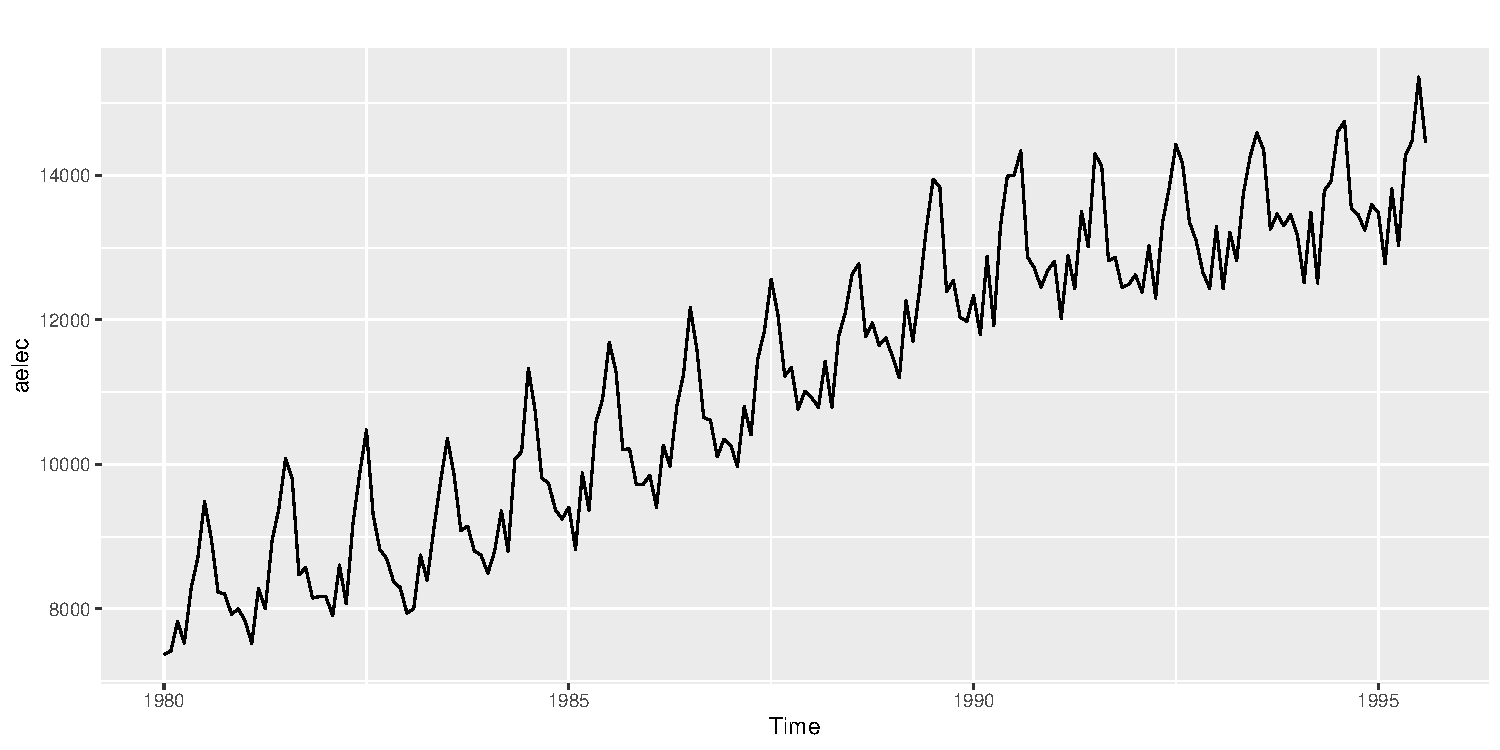
\includegraphics[keepaspectratio]{03-chap3_files/figure-pdf/unnamed-chunk-3-1.pdf}}

\begin{Shaded}
\begin{Highlighting}[]
\CommentTok{\# Plot some forecasts}
\FunctionTok{autoplot}\NormalTok{(aelec) }\SpecialCharTok{+}
  \FunctionTok{autolayer}\NormalTok{(}\FunctionTok{meanf}\NormalTok{(aelec, }\AttributeTok{h=}\DecValTok{11}\NormalTok{),}
    \AttributeTok{series=}\StringTok{"Mean"}\NormalTok{, }\AttributeTok{PI=}\ConstantTok{FALSE}\NormalTok{) }\SpecialCharTok{+}
  \FunctionTok{autolayer}\NormalTok{(}\FunctionTok{naive}\NormalTok{(aelec, }\AttributeTok{h=}\DecValTok{11}\NormalTok{),}
    \AttributeTok{series=}\StringTok{"Naïve"}\NormalTok{, }\AttributeTok{PI=}\ConstantTok{FALSE}\NormalTok{) }\SpecialCharTok{+}
  \FunctionTok{autolayer}\NormalTok{(}\FunctionTok{snaive}\NormalTok{(aelec, }\AttributeTok{h=}\DecValTok{11}\NormalTok{),}
    \AttributeTok{series=}\StringTok{"Seasonal naïve"}\NormalTok{, }\AttributeTok{PI=}\ConstantTok{FALSE}\NormalTok{) }\SpecialCharTok{+}
  \FunctionTok{ggtitle}\NormalTok{(}\StringTok{"Forecasts from Mean, NAIVE and SNAIVE"}\NormalTok{) }\SpecialCharTok{+}
  \FunctionTok{xlab}\NormalTok{(}\StringTok{"Year"}\NormalTok{) }\SpecialCharTok{+} \FunctionTok{ylab}\NormalTok{(}\StringTok{"Value"}\NormalTok{) }\SpecialCharTok{+}
  \FunctionTok{guides}\NormalTok{(}\AttributeTok{colour=}\FunctionTok{guide\_legend}\NormalTok{(}\AttributeTok{title=}\StringTok{"Forecast"}\NormalTok{))}
\end{Highlighting}
\end{Shaded}

\pandocbounded{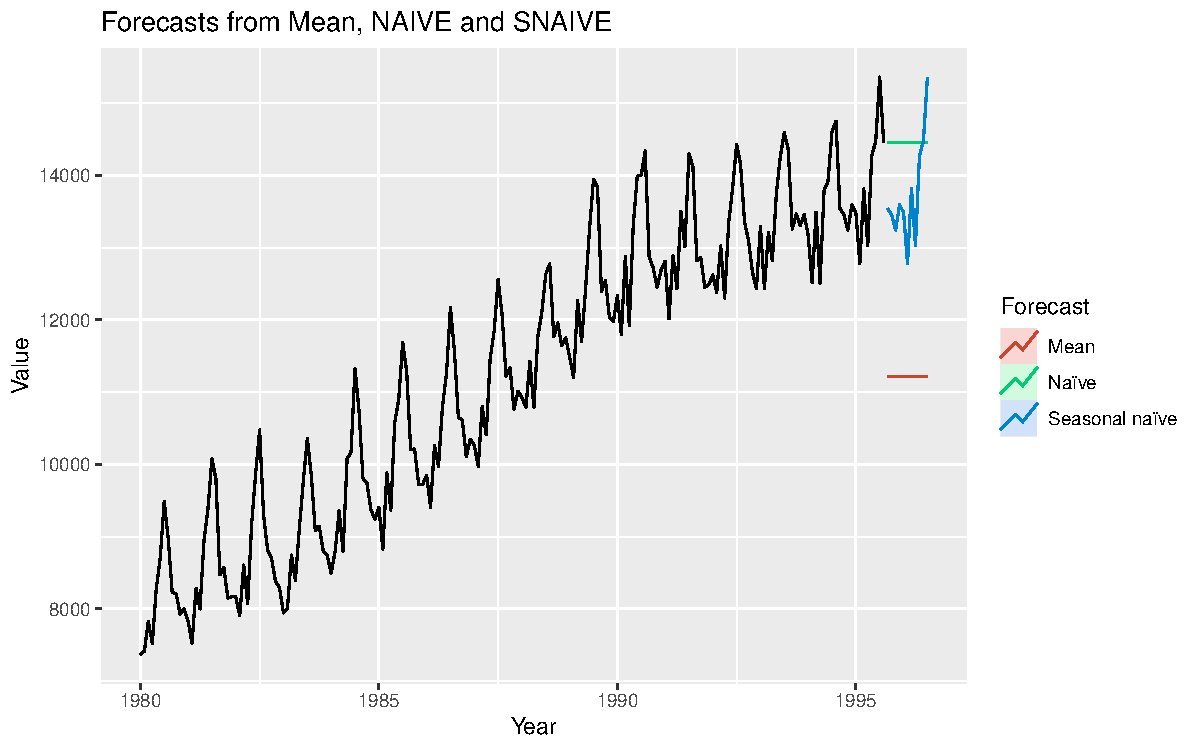
\includegraphics[keepaspectratio]{03-chap3_files/figure-pdf/unnamed-chunk-4-1.pdf}}

\section{Time Series and Stochastic
Processes}\label{time-series-and-stochastic-processes}

The terms stochastic processes and time series are closely related but
not the same.

A \textbf{stochastic process} is a collection of random variables
indexed by time (or space).

\[\{X_t : t \in T\},\]

where \(T\) is the index set (e.g., discrete or continuous time).

A \textbf{time series} is a single realization (observed data) of a
stochastic process. It is the actual sequence of observations collected
over time.

In short:

Stochastic process = model/theory (all possible sequences). The
probability mechanism (all possible paths).

Time series = observed data (one sequence). One observed path (the
single trajectory we actually have).

\section{Statistical Properties}\label{statistical-properties}

\subsection{Mean function}\label{mean-function}

Let \({X_1, X_2, ...}\) be a sequence of time index random variables.

The \textbf{mean function} of \({X_t}\) is

\[\mu_X(t)=E(X_t).\]

\subsection{Covariance function}\label{covariance-function}

The \textbf{covariance function} of \({X_t}\) is

\[\gamma_X(r, s)=Cov(X_r, X_s)=E[(X_r-\mu_X(r))(X_s-\mu_X(s))]\]

for all integers \((r)\) and \((s)\).

\subsection{Autocovariance function}\label{autocovariance-function}

The autocovariance function of \({X_t}\) at lag \((h)\) is defined by
\[\gamma_X(h):=\gamma_X(h, 0)=\gamma(t+h, t)=Cov(X_{t+h}, X_t).\]

or

The autocovariance function of \({X_t}\) at lag \((h)\) is

\[\gamma_X(h)=Cov(X_{t+h}, X_t).\]

\subsection{Autocorrelation function}\label{autocorrelation-function}

The autocorrelation function of \({X_t}\) at lag \((h)\) is

\[\rho_X(h)=\frac{\gamma_X(h)}{\gamma_X(0)}=Cor(X_{t+h}, X_t).\]

\section{Weekly stationary}\label{weekly-stationary}

A time series \({X_t}\) is called weekly stationary if

\begin{itemize}
\item
  \(\mu_X(t)\) is independent of \(t\).
\item
  \(Var(X_t) = \sigma^2\), Variance is constant. 2
\item
  \(\gamma_X(t+h, t)\) is independent of \((t)\) for each \((h)\). The
  autocovariance depends only on the lag (\(\gamma(h)\) depends only on
  how far apart two points are (\(h\)), and not on the actual time
  \(t\).
\end{itemize}

In other words the statistical properties of the time series (mean,
variance, autocorrelation, etc.) do not depend on the time at which the
series is observed, that is no trend or seasonality. However, a time
series with cyclic behaviour (but with no trend or seasonality) is
stationary.

\section{Strict stationarity of a time
series}\label{strict-stationarity-of-a-time-series}

A time series \(\{X_t\}\) is called strictly stationary if the random
vector \([X_1, X_2..., X_n]\) and \([X_{1+h}, X_{2+h}..., X_{n+h}]\)
have the same joint distribution for all integers \((h)\) and
\((n > 0)\).

\section{1. independent and identically distributed (iid)
noise}\label{independent-and-identically-distributed-iid-noise}

\begin{enumerate}
\def\labelenumi{\arabic{enumi}.}
\item
  no trend or seasonal component
\item
  observations are independent and identically distributed (iid) random
  variables with zero mean.
\item
  Notation: \({X_t} \sim IID(0, \sigma^2)\)
\item
  plays an important role as a building block for more complicated time
  series.
\end{enumerate}

\section{2. White noise}\label{white-noise}

If \({X_t}\) is a sequence of uncorrelated random variables, each with
zero mean and variance \(\sigma^2\), then such a sequence is referred to
as \textbf{white noise}.

\section{\texorpdfstring{Every \((IID(0, \sigma^2)\) sequence is
\((WN(0, \sigma^2)\) but not conversely.
Why?}{Every (IID(0, \textbackslash sigma\^{}2) sequence is (WN(0, \textbackslash sigma\^{}2) but not conversely. Why?}}\label{every-iid0-sigma2-sequence-is-wn0-sigma2-but-not-conversely.-why}

\subsection{1. White Noise (WN)}\label{white-noise-wn}

A sequence \(\{X_t\}\) is called \textbf{white noise} with mean \(0\)
and variance \(\sigma^2\), written \(WN(0, \sigma^2)\), if:

\begin{itemize}
\tightlist
\item
  \(\mathbb{E}[X_t] = 0\) for all \(t\).\\
\item
  \(\mathrm{Var}(X_t) = \sigma^2\) for all \(t\).\\
\item
  \(\mathrm{Cov}(X_t, X_s) = 0\) for all \(t \neq s\) (uncorrelated
  across time).
\end{itemize}

Notice: \emph{uncorrelated \(\neq\) independent}.

\subsection{\texorpdfstring{2. i.i.d.
\((0, \sigma^2)\)}{2. i.i.d. (0, \textbackslash sigma\^{}2)}}\label{i.i.d.-0-sigma2}

A sequence \(\{X_t\}\) is \(IID(0, \sigma^2)\) if:

\begin{itemize}
\tightlist
\item
  \(\mathbb{E}[X_t] = 0\).\\
\item
  \(\mathrm{Var}(X_t) = \sigma^2\).\\
\item
  \(X_t\) are independent and identically distributed.
\end{itemize}

\subsection{\texorpdfstring{3. Why every \(IID(0, \sigma^2)\) is
\(WN(0, \sigma^2)\)}{3. Why every IID(0, \textbackslash sigma\^{}2) is WN(0, \textbackslash sigma\^{}2)}}\label{why-every-iid0-sigma2-is-wn0-sigma2}

\begin{itemize}
\tightlist
\item
  Independence \(\;\Rightarrow\;\) zero correlation.\\
\item
  So, an i.i.d. sequence automatically satisfies the white noise
  conditions (same mean, same variance, no correlation).
\end{itemize}

Therefore:

\[
IID(0, \sigma^2) \;\;\Rightarrow\;\; WN(0, \sigma^2).
\]

\subsection{4. Why not conversely?}\label{why-not-conversely}

The reverse is not always true, because \textbf{white noise only
requires uncorrelatedness, not full independence}.

That means a sequence could be white noise but still have dependence in
higher moments (nonlinear dependence).

\section{5. Example of WN but not IID}\label{example-of-wn-but-not-iid}

Let \(\{Z_t\}\) be i.i.d. \(N(0,1)\). Define

\[
X_t = Z_t \cdot Z_{t-1}.
\]

Then:

\begin{itemize}
\tightlist
\item
  \(\mathbb{E}[X_t] = 0\),\\
\item
  \(\mathrm{Var}(X_t) = 1\),\\
\item
  For \(t \neq s\), \(\mathrm{Cov}(X_t, X_s) = 0\). ✅ So it's white
  noise.
\end{itemize}

But the sequence is \textbf{not independent} (because \(X_t\) depends on
\(Z_{t-1}\), which also appears in \(X_{t-1}\)).

Thus,

\[
X_t \sim WN(0,1) \quad \text{but not} \quad IID(0,1).
\]

\section{Simulation example}\label{simulation-example}

IID series

\begin{Shaded}
\begin{Highlighting}[]
\FunctionTok{set.seed}\NormalTok{(}\DecValTok{123}\NormalTok{)}

\CommentTok{\# Parameters}
\NormalTok{n }\OtherTok{\textless{}{-}} \DecValTok{200}        \CommentTok{\# length of series}
\NormalTok{sigma }\OtherTok{\textless{}{-}} \DecValTok{1}      \CommentTok{\# standard deviation}

\CommentTok{\# IID(0, sigma\^{}2) \textasciitilde{} Normal(0, sigma\^{}2)}
\NormalTok{iid\_seq }\OtherTok{\textless{}{-}} \FunctionTok{rnorm}\NormalTok{(n, }\AttributeTok{mean =} \DecValTok{0}\NormalTok{, }\AttributeTok{sd =}\NormalTok{ sigma)}

\CommentTok{\# Quick check}
\FunctionTok{mean}\NormalTok{(iid\_seq)      }\CommentTok{\# should be \textasciitilde{}0}
\end{Highlighting}
\end{Shaded}

\begin{verbatim}
[1] -0.008570445
\end{verbatim}

\begin{Shaded}
\begin{Highlighting}[]
\FunctionTok{var}\NormalTok{(iid\_seq)       }\CommentTok{\# should be \textasciitilde{}sigma\^{}2}
\end{Highlighting}
\end{Shaded}

\begin{verbatim}
[1] 0.8895506
\end{verbatim}

\begin{Shaded}
\begin{Highlighting}[]
\FunctionTok{acf}\NormalTok{(iid\_seq)       }\CommentTok{\# autocorrelations \textasciitilde{} 0}
\end{Highlighting}
\end{Shaded}

\pandocbounded{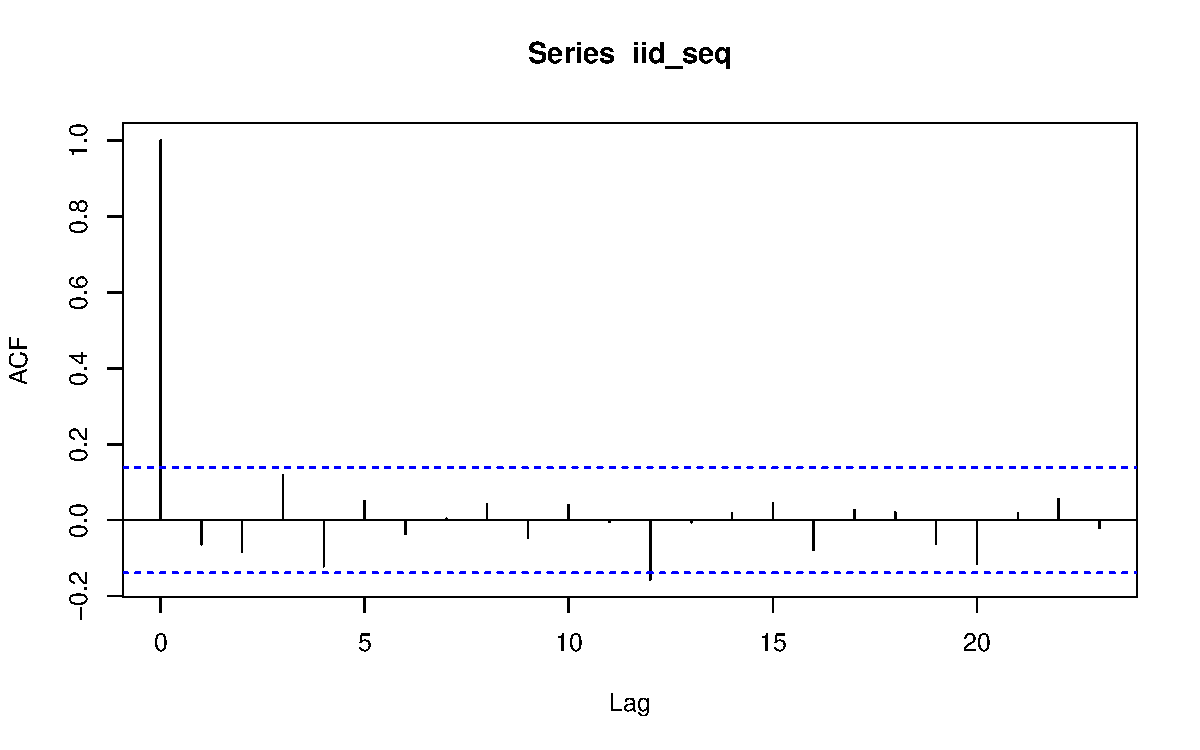
\includegraphics[keepaspectratio]{03-chap3_files/figure-pdf/unnamed-chunk-5-1.pdf}}

White noise

\begin{Shaded}
\begin{Highlighting}[]
\FunctionTok{set.seed}\NormalTok{(}\DecValTok{123}\NormalTok{)}

\NormalTok{n }\OtherTok{\textless{}{-}} \DecValTok{200}
\NormalTok{Z }\OtherTok{\textless{}{-}} \FunctionTok{rnorm}\NormalTok{(n, }\AttributeTok{mean =} \DecValTok{0}\NormalTok{, }\AttributeTok{sd =} \DecValTok{1}\NormalTok{)}

\CommentTok{\# Construct WN but not IID}
\NormalTok{wn\_not\_iid }\OtherTok{\textless{}{-}}\NormalTok{ Z[}\SpecialCharTok{{-}}\DecValTok{1}\NormalTok{] }\SpecialCharTok{*}\NormalTok{ Z[}\SpecialCharTok{{-}}\NormalTok{n]   }\CommentTok{\# X\_t = Z\_t * Z\_\{t{-}1\}, length n{-}1}

\CommentTok{\# Quick check}
\FunctionTok{mean}\NormalTok{(wn\_not\_iid)        }\CommentTok{\# \textasciitilde{}0}
\end{Highlighting}
\end{Shaded}

\begin{verbatim}
[1] -0.05650406
\end{verbatim}

\begin{Shaded}
\begin{Highlighting}[]
\FunctionTok{var}\NormalTok{(wn\_not\_iid)         }\CommentTok{\# \textasciitilde{}1}
\end{Highlighting}
\end{Shaded}

\begin{verbatim}
[1] 0.8196189
\end{verbatim}

\begin{Shaded}
\begin{Highlighting}[]
\FunctionTok{acf}\NormalTok{(wn\_not\_iid)         }\CommentTok{\# uncorrelated {-}\textgreater{} ACF \textasciitilde{} 0}
\end{Highlighting}
\end{Shaded}

\pandocbounded{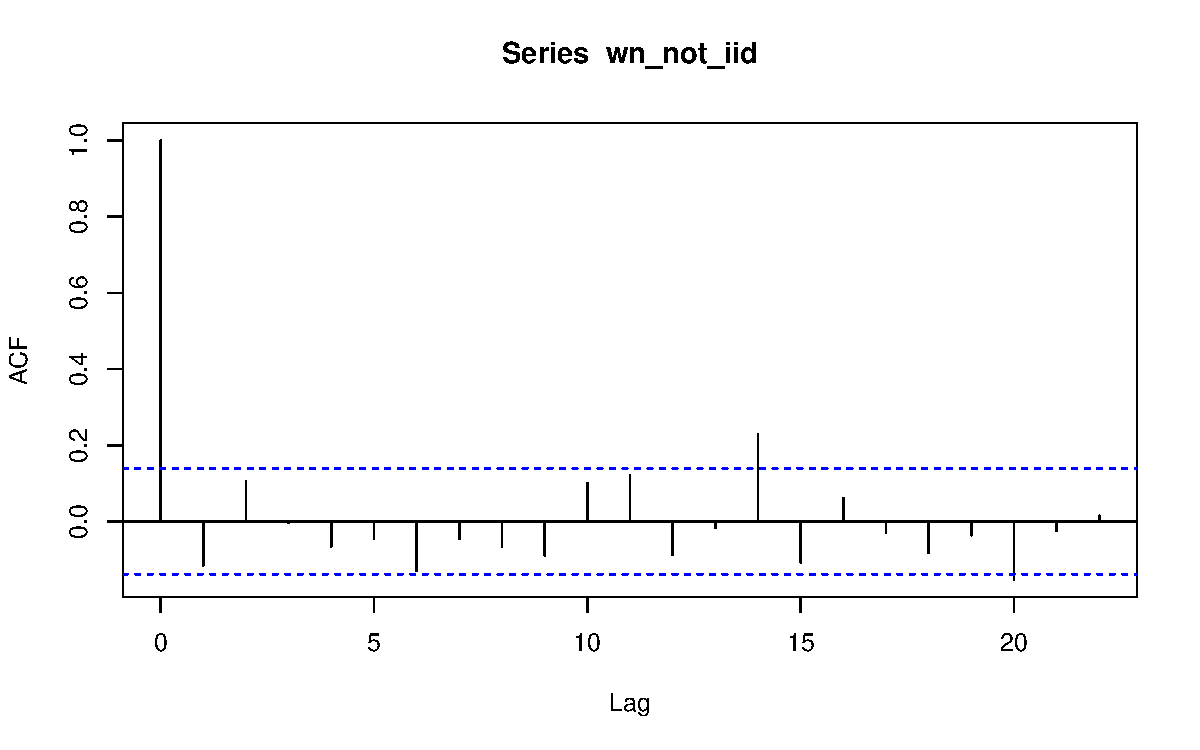
\includegraphics[keepaspectratio]{03-chap3_files/figure-pdf/unnamed-chunk-6-1.pdf}}

Side-by-side visualisation

\pandocbounded{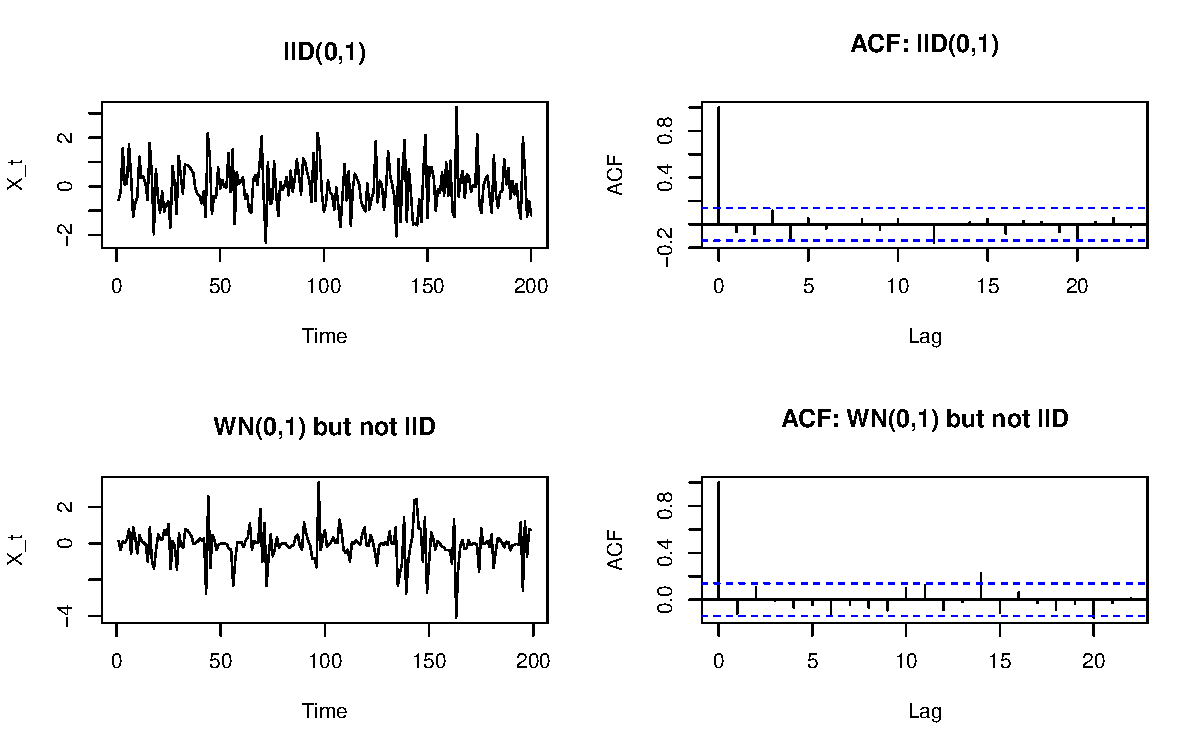
\includegraphics[keepaspectratio]{03-chap3_files/figure-pdf/unnamed-chunk-7-1.pdf}}

\section{3. Random walk}\label{random-walk}

A random walk process is obtained by cumulatively summing iid random
variables. If \({S_t, t=0, 1, 2, ...}\) is a random walk process, then
\(S_0 =0\)

\(S_1=0+X_1\)

\(S_2=0+X_1+X_2\)

\(...\)

\(S_t=X_1+X_2+...+X_t.\)

\textbf{Question}

Is \({S_t, t=0, 1, 2, ...}\) a weak stationary process?

\section{Identifying non-stationarity in the
mean}\label{identifying-non-stationarity-in-the-mean}

\begin{itemize}
\item
  Using time series plot
\item
  ACF plot

  \begin{itemize}
  \item
    ACF of stationary time series will drop to relatively quickly.
  \item
    The ACF of non-stationary series decreases slowly.
  \item
    For non-stationary series, the ACF at lag 1 is often large and
    positive.
  \end{itemize}
\end{itemize}

\section{Backshift notation:}\label{backshift-notation}

\[BX_t=X_{t-1}\]

\section{Ordinary differencing}\label{ordinary-differencing}

The first-order differencing can be defined as

\[\nabla X_t = X_t-X_{t-1}=X_t-BX_t=(1-B)X_t\] where \(\nabla=1-B\).

The second-order differencing

\[\nabla^2X_t=\nabla(\nabla X_t)=\nabla(X_t-X_{t-1})=\nabla X_t - \nabla X_{t-1}\]

\[\nabla X_t - \nabla X_{t-1}=(X_t-X_{t-1})-(X_{t-1}-X_{t-2})\]

In practice, we seldom need to go beyond second order differencing.

\section{Seasonal differencing}\label{seasonal-differencing}

Differencing between an observation and the corresponding observation
from the previous year.

\[\nabla_mX_t=X_t-X_{t-m}=(1-B^m)X_t\] where \((m)\) is the number of
seasons. For monthly, \((m=12)\), for quarterly \((m=4)\).

For monthly series

\[\nabla_{12}X_t=X_t-X_{t-12}\]

\section{Twice-differenced series}\label{twice-differenced-series}

\[\nabla^2_{12}X_t=\nabla_{12}X_t-\nabla_{12}X_{t-1}\]
\[\nabla_{12}X_t-\nabla_{12}X_{t-1}=(X_t-X_{t-12})-(X_{t-1}-X_{t-13})\]
If seasonality is strong, the seasonal differencing should be done
first.

\section{Deterministic trend vs Stochastic
trend}\label{deterministic-trend-vs-stochastic-trend}

\subsection{Deterministic trend}\label{deterministic-trend}

\[Y_t  = f(t) + \epsilon_t\]

where \(\epsilon_t \sim iid(0, \sigma^2)\), \(t = 1, 2, ...T\)

Mean of the process is time dependent, but the variance of the process
is constant.

A trend is deterministic if it is a nonrandom function of time. A
deterministic trend is a predictable, fixed function of time. If you
know the form of the function, you can determine the trend exactly.

\subsection{Stochastic trend}\label{stochastic-trend}

A stochastic trend is driven by random shocks that accumulate over time.
A stochastic trend is driven by random shocks (also called innovations,
disturbances, or error terms) that accumulate over time.

\textbf{1. Random walk}

\[Y_t = Y_{t-1} + \epsilon_t\]

\begin{itemize}
\item
  Random walk has a stochastic trend.
\item
  Model behind naive method.
\end{itemize}

A trend is said to be stochastic if it is a random function of time.

\textbf{2. Random walk with drift}

\[Y_t = \alpha +  Y_{t-1} + \epsilon_t\]

\begin{itemize}
\item
  Random walk with drift has a stochastic trend and a deterministic
  trend.
\item
  Model behind drift method.
\end{itemize}

\section{Random walk}\label{random-walk-1}

\[
\begin{aligned}
  Y_t &= Y_{t-1} + \epsilon_t \\
     Y_1    &= Y_0 + \epsilon_1 \\
         Y_2 &=  Y_1 + \epsilon_2=Y_0 + \epsilon_1 + \epsilon_2\\
          Y_3 &=  Y_2 + \epsilon_3=Y_0 + \epsilon_1 + \epsilon_2 +\epsilon_3\\
          .   \\
          Y_t &=Y_{t-1} + \epsilon_t=Y_0 + \epsilon_1 + \epsilon_2 + \epsilon_3 +...+ \epsilon_t = Y_0 + \sum_{i=1}^{t} \epsilon_t
\end{aligned}
\]

Mean: \(E(Y_t) = Y_0\).

Variance: \(Var(Y_t)=t \sigma^2\).

\section{Random walk with drift}\label{random-walk-with-drift}

\[
\begin{aligned}
  Y_t &= \alpha + Y_{t-1} + \epsilon_t \\
     Y_1    &= \alpha+Y_0 + \epsilon_1 \\
         Y_2 &= \alpha+ Y_1 + \epsilon_2=2 \alpha+Y_0 + \epsilon_1 + \epsilon_2\\
          Y_3 &= \alpha+ Y_2 + \epsilon_3= 3 \alpha+ Y_0 + \epsilon_1 + \epsilon_2 +\epsilon_3\\
          .   \\
          Y_t &= \alpha+Y_{t-1} + \epsilon_t= t \alpha+ Y_0 + \epsilon_1 + \epsilon_2 + \epsilon_3 +...+ \epsilon_t \\
          Y_t &= t \alpha + Y_0 + \sum_{i=1}^{t} \epsilon_t
\end{aligned}
\]

It has a \emph{deterministic trend} \((Y_0 + t \alpha)\) and a
\emph{stochastic trend} \(\sum_{i=1}^{t} \epsilon_t\).

Mean: \(E(Y_t) = Y_0 + t\alpha\)

Variance: \(Var(Y_t) = t\sigma^2\).

There is a trend in both mean and variance.

\section{Common trend removal (de-trending)
procedures}\label{common-trend-removal-de-trending-procedures}

\begin{enumerate}
\def\labelenumi{\arabic{enumi}.}
\item
  Deterministic trend: Time-trend regression

  The trend can be removed by fitting a deterministic polynomial time
  trend. The residual series after removing the trend will give us the
  de-trended series.
\item
  Stochastic trend: Differencing

  The process is also known as a \textbf{Difference-stationary process}.
\end{enumerate}

\section{Remove seasonality}\label{remove-seasonality}

Take seasonal differencing

\section{Example: Differencing on AirPassengers
Data}\label{example-differencing-on-airpassengers-data}

The built-in AirPassengers dataset (monthly airline passengers,
1949--1960) has trend + seasonality.

\begin{Shaded}
\begin{Highlighting}[]
\CommentTok{\# Load data}
\FunctionTok{data}\NormalTok{(}\StringTok{"AirPassengers"}\NormalTok{)}
\NormalTok{ts\_data }\OtherTok{\textless{}{-}}\NormalTok{ AirPassengers}

\CommentTok{\#par(mfrow = c(3,2))}

\CommentTok{\# 1. Original series}
\FunctionTok{plot}\NormalTok{(ts\_data, }\AttributeTok{main =} \StringTok{"Original Series"}\NormalTok{, }\AttributeTok{ylab =} \StringTok{"Passengers"}\NormalTok{)}
\end{Highlighting}
\end{Shaded}

\pandocbounded{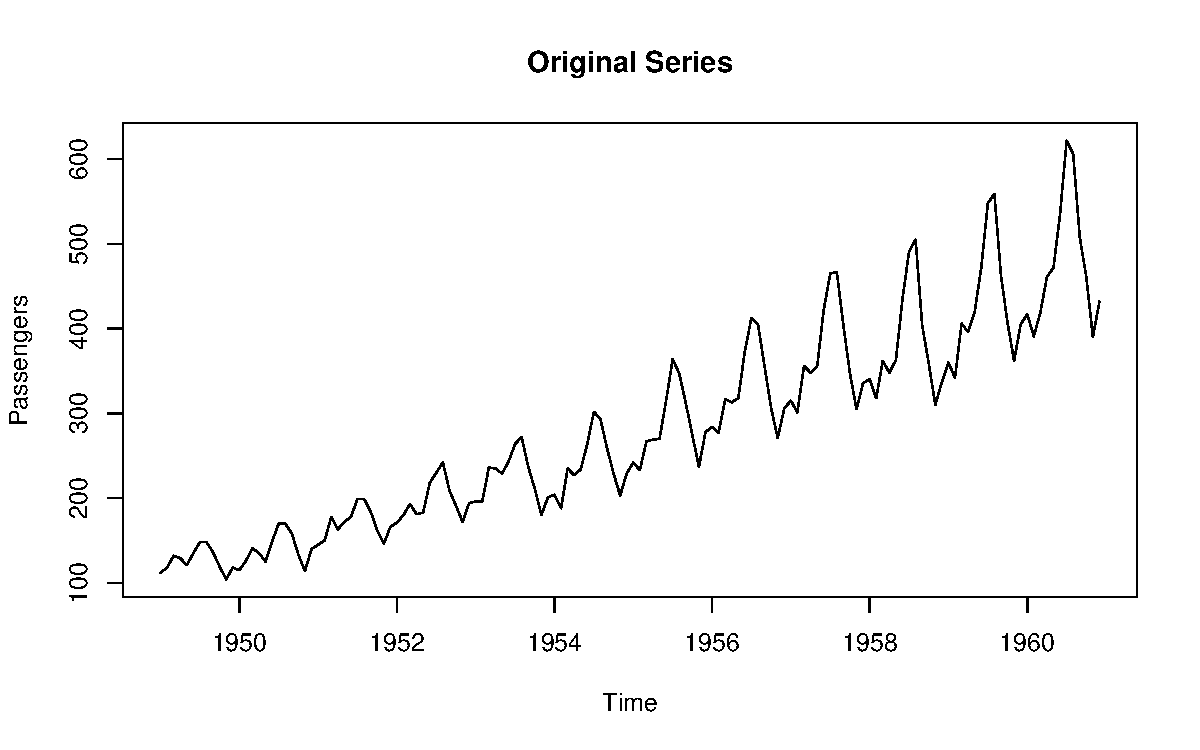
\includegraphics[keepaspectratio]{03-chap3_files/figure-pdf/unnamed-chunk-8-1.pdf}}

\begin{Shaded}
\begin{Highlighting}[]
\FunctionTok{acf}\NormalTok{(ts\_data, }\AttributeTok{main =} \StringTok{"ACF: Original Series"}\NormalTok{)}
\end{Highlighting}
\end{Shaded}

\pandocbounded{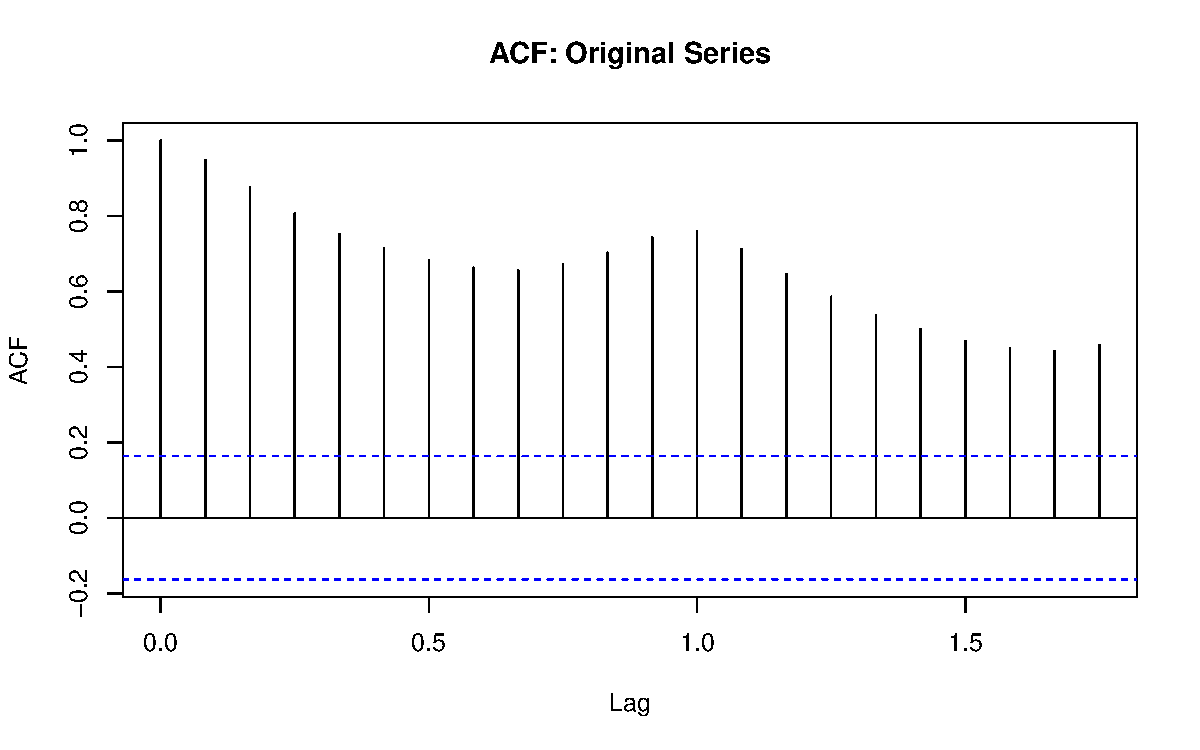
\includegraphics[keepaspectratio]{03-chap3_files/figure-pdf/unnamed-chunk-8-2.pdf}}

\begin{Shaded}
\begin{Highlighting}[]
\CommentTok{\# 2. First difference (remove trend)}
\NormalTok{diff1 }\OtherTok{\textless{}{-}} \FunctionTok{diff}\NormalTok{(ts\_data, }\AttributeTok{differences =} \DecValTok{1}\NormalTok{)}
\FunctionTok{plot}\NormalTok{(diff1, }\AttributeTok{main =} \StringTok{"1st Difference (Remove Trend)"}\NormalTok{, }\AttributeTok{ylab =} \StringTok{"Difference"}\NormalTok{)}
\end{Highlighting}
\end{Shaded}

\pandocbounded{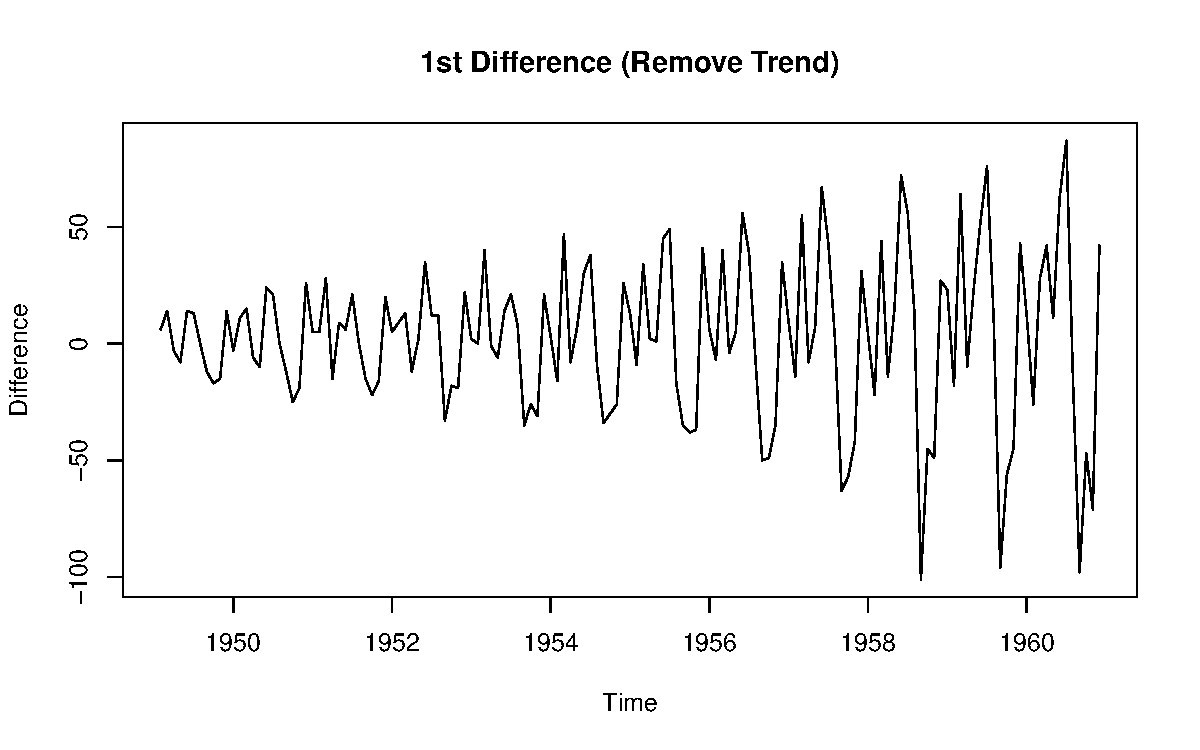
\includegraphics[keepaspectratio]{03-chap3_files/figure-pdf/unnamed-chunk-8-3.pdf}}

\begin{Shaded}
\begin{Highlighting}[]
\FunctionTok{acf}\NormalTok{(diff1, }\AttributeTok{main =} \StringTok{"ACF: 1st Difference"}\NormalTok{)}
\end{Highlighting}
\end{Shaded}

\pandocbounded{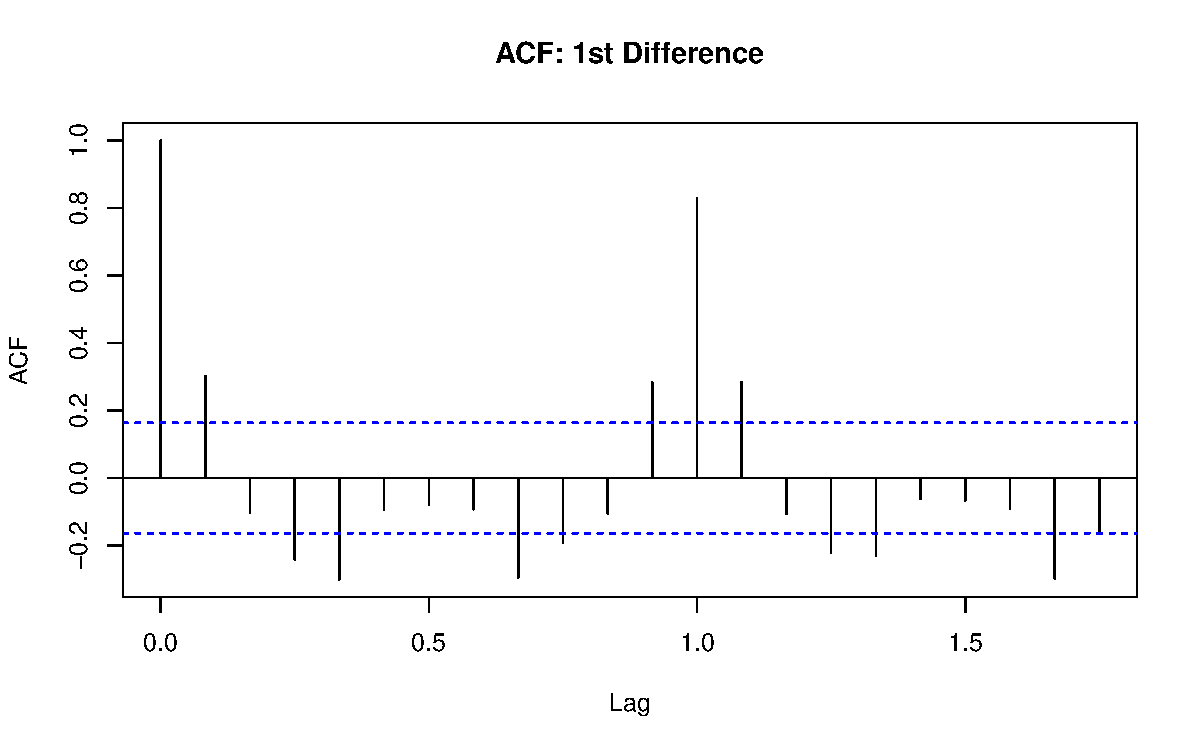
\includegraphics[keepaspectratio]{03-chap3_files/figure-pdf/unnamed-chunk-8-4.pdf}}

\begin{Shaded}
\begin{Highlighting}[]
\CommentTok{\# 3. Seasonal difference (lag = 12, remove seasonality)}
\NormalTok{diff\_seasonal }\OtherTok{\textless{}{-}} \FunctionTok{diff}\NormalTok{(diff1, }\AttributeTok{lag =} \DecValTok{12}\NormalTok{)}
\FunctionTok{plot}\NormalTok{(diff\_seasonal, }\AttributeTok{main =} \StringTok{"Seasonal Difference (Remove Seasonality)"}\NormalTok{, }\AttributeTok{ylab =} \StringTok{"Difference"}\NormalTok{)}
\end{Highlighting}
\end{Shaded}

\pandocbounded{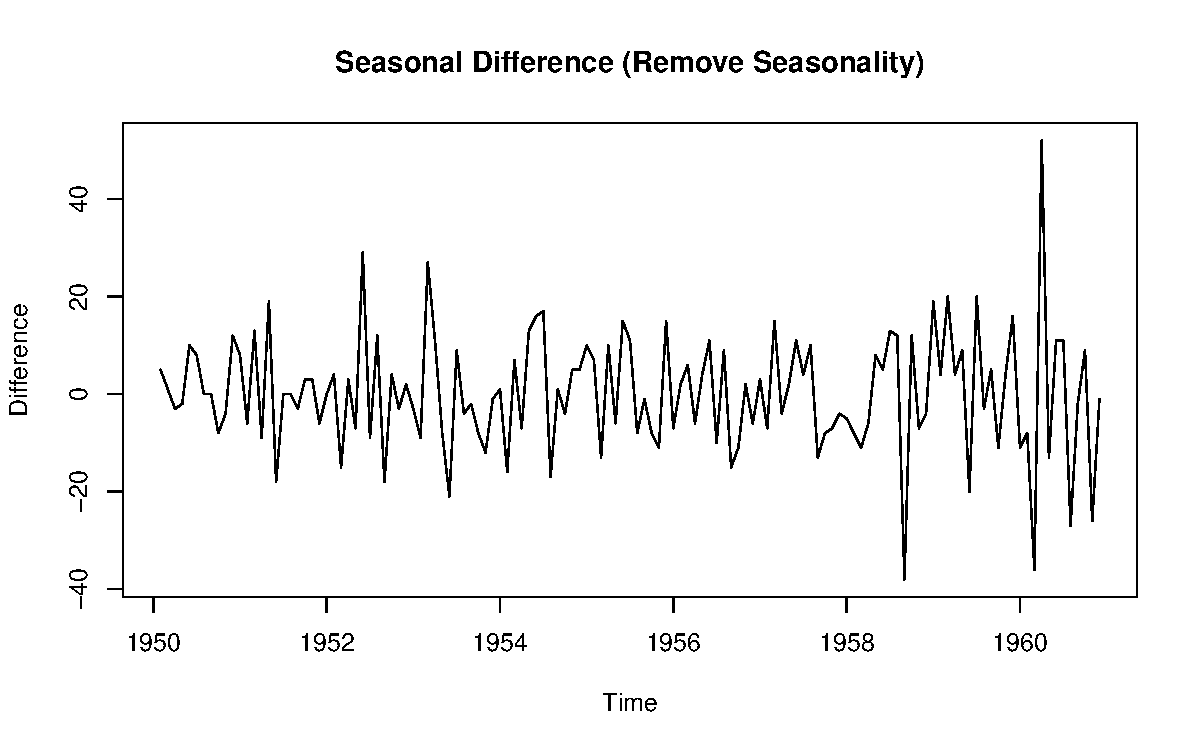
\includegraphics[keepaspectratio]{03-chap3_files/figure-pdf/unnamed-chunk-8-5.pdf}}

\begin{Shaded}
\begin{Highlighting}[]
\FunctionTok{acf}\NormalTok{(diff\_seasonal, }\AttributeTok{main =} \StringTok{"ACF: Seasonal Difference"}\NormalTok{)}
\end{Highlighting}
\end{Shaded}

\pandocbounded{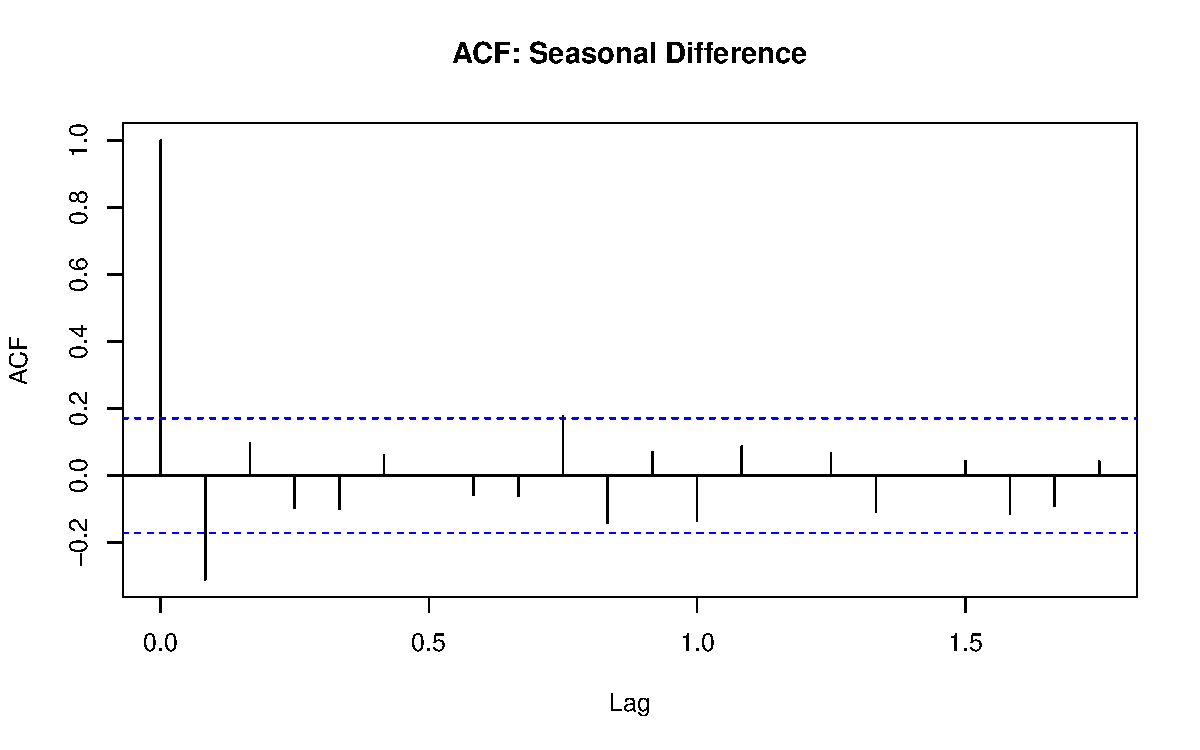
\includegraphics[keepaspectratio]{03-chap3_files/figure-pdf/unnamed-chunk-8-6.pdf}}

\begin{Shaded}
\begin{Highlighting}[]
\CommentTok{\# 3. Seasonal difference (lag = 12, remove seasonality from the original series)}
\NormalTok{diff\_seasonal\_only }\OtherTok{\textless{}{-}} \FunctionTok{diff}\NormalTok{(ts\_data, }\AttributeTok{lag =} \DecValTok{12}\NormalTok{)}
\FunctionTok{plot}\NormalTok{(diff\_seasonal\_only, }\AttributeTok{main =} \StringTok{"Seasonal Difference (Remove Seasonality)"}\NormalTok{, }\AttributeTok{ylab =} \StringTok{"Difference"}\NormalTok{)}
\end{Highlighting}
\end{Shaded}

\pandocbounded{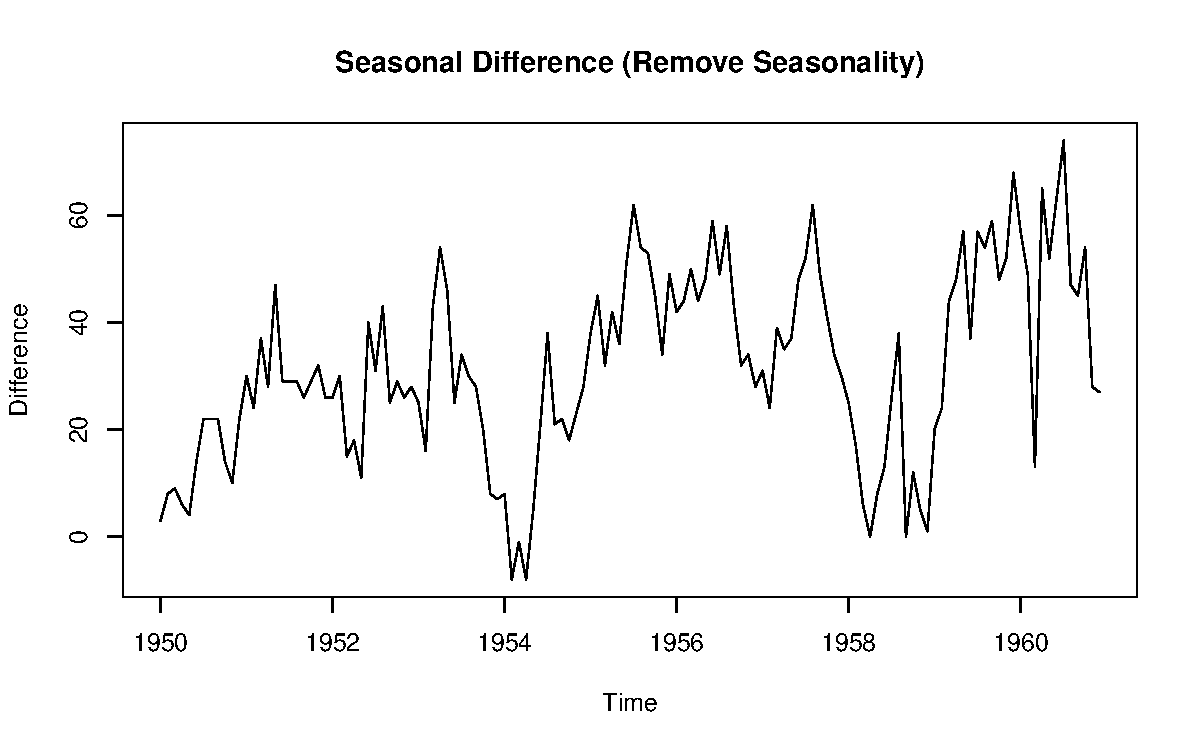
\includegraphics[keepaspectratio]{03-chap3_files/figure-pdf/unnamed-chunk-8-7.pdf}}

\begin{Shaded}
\begin{Highlighting}[]
\FunctionTok{acf}\NormalTok{(diff\_seasonal\_only, }\AttributeTok{main =} \StringTok{"ACF: Seasonal Difference"}\NormalTok{)}
\end{Highlighting}
\end{Shaded}

\pandocbounded{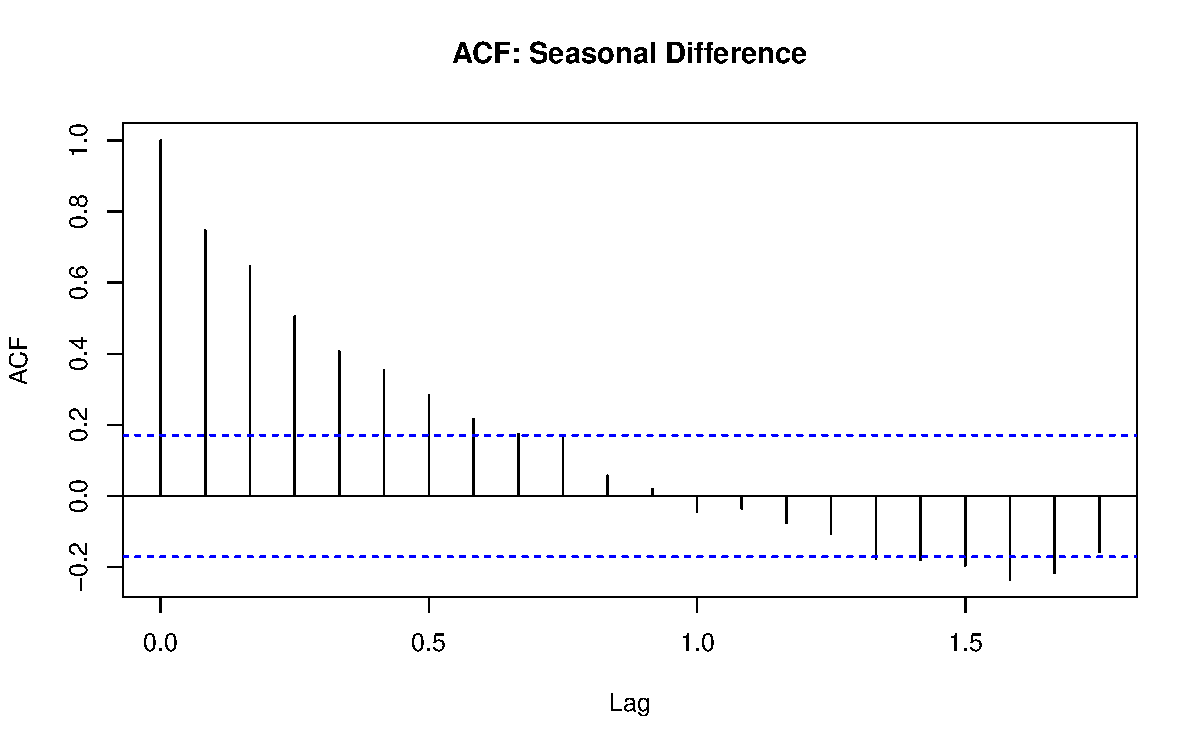
\includegraphics[keepaspectratio]{03-chap3_files/figure-pdf/unnamed-chunk-8-8.pdf}}

\begin{Shaded}
\begin{Highlighting}[]
\FunctionTok{head}\NormalTok{(ts\_data, }\DecValTok{14}\NormalTok{)}
\end{Highlighting}
\end{Shaded}

\begin{verbatim}
     Jan Feb Mar Apr May Jun Jul Aug Sep Oct Nov Dec
1949 112 118 132 129 121 135 148 148 136 119 104 118
1950 115 126                                        
\end{verbatim}

\begin{Shaded}
\begin{Highlighting}[]
\FunctionTok{head}\NormalTok{(diff1, }\DecValTok{14}\NormalTok{)}
\end{Highlighting}
\end{Shaded}

\begin{verbatim}
     Jan Feb Mar Apr May Jun Jul Aug Sep Oct Nov Dec
1949       6  14  -3  -8  14  13   0 -12 -17 -15  14
1950  -3  11  15                                    
\end{verbatim}

\begin{Shaded}
\begin{Highlighting}[]
\FunctionTok{head}\NormalTok{(diff\_seasonal, }\DecValTok{14}\NormalTok{)}
\end{Highlighting}
\end{Shaded}

\begin{verbatim}
     Jan Feb Mar Apr May Jun Jul Aug Sep Oct Nov Dec
1950       5   1  -3  -2  10   8   0   0  -8  -4  12
1951   8  -6  13                                    
\end{verbatim}

\begin{Shaded}
\begin{Highlighting}[]
\FunctionTok{head}\NormalTok{(diff\_seasonal\_only, }\DecValTok{14}\NormalTok{)}
\end{Highlighting}
\end{Shaded}

\begin{verbatim}
     Jan Feb Mar Apr May Jun Jul Aug Sep Oct Nov Dec
1950   3   8   9   6   4  14  22  22  22  14  10  22
1951  30  24                                        
\end{verbatim}

\section{Notation: I(d)}\label{notation-id}

Integrated to order \(d\): Series can be made stationary by differencing
\(d\) times.

\begin{itemize}
\tightlist
\item
  Known as \(I(d)\) process.
\end{itemize}

\textbf{Question:} Show that random walk process is an \(I(1)\) process.

The random walk process is called a unit root process. (If one of the
roots turns out to be one, then the process is called unit root
process.)

\section{Variance stabilization}\label{variance-stabilization}

Transform the series.

Eg:

\begin{itemize}
\item
  Square root: \(W_t = \sqrt{Y_t}\)
\item
  Logarithm: \(W_t = log({Y_t})\)

  \begin{itemize}
  \item
    This very useful.
  \item
    Interpretable: Changes in a log value are \textbf{relative (percent)
    changes on the original sclae}.
  \end{itemize}
\end{itemize}

\begin{Shaded}
\begin{Highlighting}[]
\NormalTok{log\_ts }\OtherTok{\textless{}{-}} \FunctionTok{log}\NormalTok{(ts\_data)}
\FunctionTok{plot}\NormalTok{(log\_ts, }\AttributeTok{main =} \StringTok{"Log{-}Transformed Series"}\NormalTok{, }\AttributeTok{ylab =} \StringTok{"log(Passengers)"}\NormalTok{, }\AttributeTok{col =} \StringTok{"steelblue"}\NormalTok{)}
\end{Highlighting}
\end{Shaded}

\pandocbounded{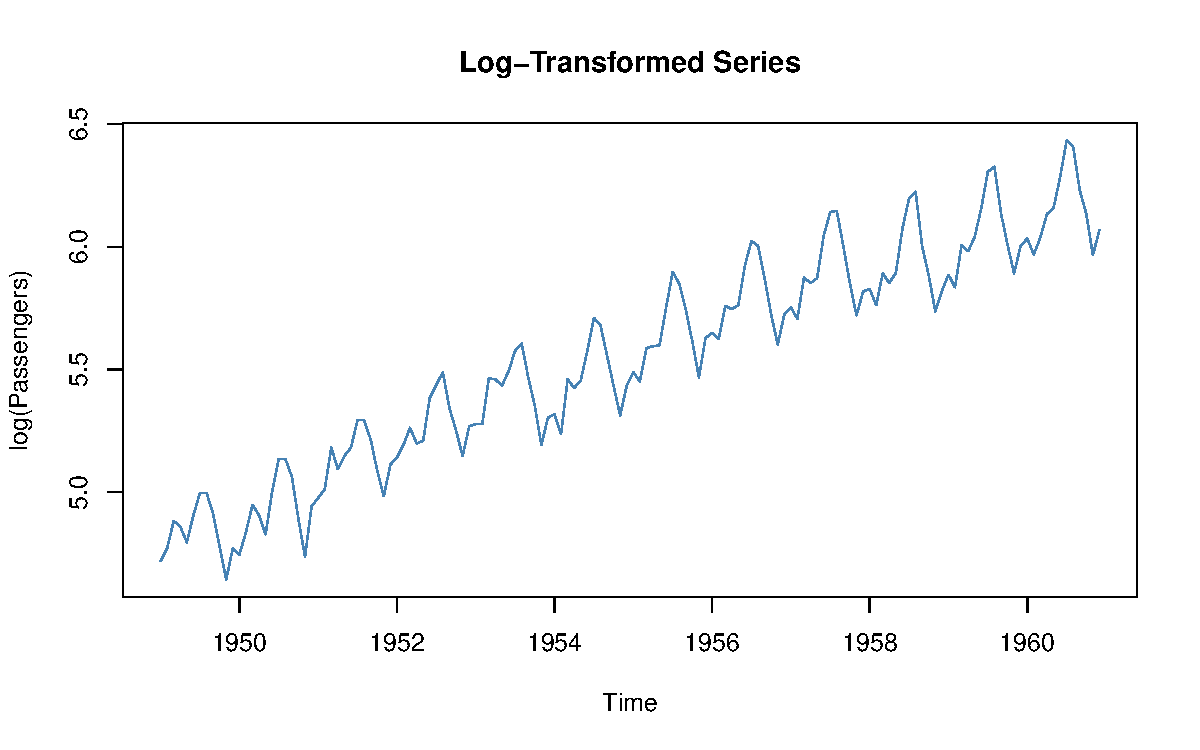
\includegraphics[keepaspectratio]{03-chap3_files/figure-pdf/unnamed-chunk-10-1.pdf}}

\bookmarksetup{startatroot}

\chapter{Models For Stationary Time
Series}\label{models-for-stationary-time-series}

In this chapter we will discuss family of autoregressive moving average
(ARMA) time series models.

\section{General Linear Process}\label{general-linear-process}

A \textbf{linear process} is a time series written as an infinite linear
combination of random shocks \(\{\varepsilon_t\}\):

\[X_t = \mu + \sum_{j=0}^{\infty} \psi_j \, \varepsilon_{t-j},\]

where,

\(\mu\) is the mean

\(\{\psi_j\}\) are coefficients (weights)

\(\varepsilon_t \sim \text{i.i.d. } (0, \sigma^2)\) are white noise
shocks.

\section{Moving Average Processes}\label{moving-average-processes}

If only finitely many coefficients \(\psi_j\) are nonzero, say up to lag
\(q\), then we have an MA(\(q\)) process:

\[X_t = \mu + \varepsilon_t + \theta_1 \varepsilon_{t-1} + \dots + \theta_q \varepsilon_{t-q},\]

where:

\begin{itemize}
\item
  \(\mu\) is the mean,
\item
  \(\varepsilon_t \sim \text{i.i.d. }(0, \sigma^2)\) are white noise
  shocks,
\item
  \(\theta_1, \dots, \theta_q\) are the MA coefficients.
\end{itemize}

So we can write:

\[\text{MA}(q) \subset \text{Linear Process}.\]

\section{Autoregressive Processes}\label{autoregressive-processes}

\(Y_t = \alpha + \phi_1 Y_{t-1} + \phi_2 Y_{t-2} + \dots + \phi_p Y_{t-p} + \epsilon_t\)

Where:

\(Y_t\) is the value at time \(t\)

\(\alpha\) is a constant,

\(\phi_1, \phi_2,...\phi_p\) are the parameters,

\(\epsilon_t\) is white noise (error term),

\(p\) is the order of the AR model.

\section{AR processes are also just special cases of the general linear
process}\label{ar-processes-are-also-just-special-cases-of-the-general-linear-process}

If the AR process is causal (i.e., roots of the characteristic
polynomial lie outside the unit circle), then it can be written as an
infinite linear process:

\[X_t = \sum_{j=0}^{\infty} \psi_j \, \varepsilon_{t-j},\]

where:

\begin{itemize}
\item
  \(\varepsilon_t \sim \text{i.i.d. }(0, \sigma^2)\) are white noise
  shocks,
\item
  \(\psi_j\) are coefficients determined from the AR parameters.
\end{itemize}

\subsection{AR(p) Process as an Infinite Linear Process Using Backshift
Operator}\label{arp-process-as-an-infinite-linear-process-using-backshift-operator}

Start with the AR(p) process:

\[X_t = \phi_1 X_{t-1} + \phi_2 X_{t-2} + \dots + \phi_p X_{t-p} + \varepsilon_t,\]

where \(\varepsilon_t \sim \text{i.i.d. }(0, \sigma^2)\) are white noise
shocks.

\subsubsection{1. Define the backshift operator
(B)}\label{define-the-backshift-operator-b}

\[B X_t = X_{t-1}, \quad B^2 X_t = X_{t-2}, \dots, B^p X_t = X_{t-p}.\]

\subsubsection{2. Rewrite the AR(p) process using
(B)}\label{rewrite-the-arp-process-using-b}

\[X_t - \phi_1 B X_t - \phi_2 B^2 X_t - \dots - \phi_p B^p X_t = \varepsilon_t\]

Factor out \(X_t\):

\[(1 - \phi_1 B - \phi_2 B^2 - \dots - \phi_p B^p) X_t = \varepsilon_t\]

Define the AR polynomial:

\[\phi(B) = 1 - \phi_1 B - \phi_2 B^2 - \dots - \phi_p B^p\]

Then the AR(p) process becomes:

\[\phi(B) X_t = \varepsilon_t\]

\subsubsection{3. Express as an infinite linear
process}\label{express-as-an-infinite-linear-process}

If the AR process is \textbf{causal} (roots of \(\phi(z)=0\) lie outside
the unit circle), we can invert the operator:

\[X_t = \phi(B)^{-1} \varepsilon_t\]

Expanding gives:

\[X_t = \sum_{j=0}^{\infty} \psi_j \, \varepsilon_{t-j},\]

where the coefficients \(\psi_j\) are determined recursively from the AR
parameters \(\phi_1, \dots, \phi_p\).

This shows that causal AR processes are \textbf{special cases of the
general linear process}.

\section{In-class: Properties of AR(1)
process}\label{in-class-properties-of-ar1-process}

Derive

\begin{itemize}
\item
  Mean
\item
  Variance
\item
  Covariance
\item
  Autocorrelation function of an AR(1) process
\end{itemize}

\section{In-class: Properties of AR(2)
process}\label{in-class-properties-of-ar2-process}

Derive

\begin{itemize}
\item
  Mean
\item
  Variance
\item
  Covariance
\item
  Autocorrelation function of an AR(1) process
\end{itemize}

\section{In-class: Properties of AR(P)
process}\label{in-class-properties-of-arp-process}

Derive

\begin{itemize}
\item
  Mean
\item
  Variance
\item
  Covariance
\item
  Autocorrelation function of an AR(P) process
\end{itemize}

\section{Properties of AR(1) model}\label{properties-of-ar1-model}

Consider the following \(AR(1)\) model.

\begin{equation}
  \label{eq:ar}
Y_t=\phi_0+\phi_1Y_{t-1}+\epsilon_{t}
\end{equation}

where \({\epsilon_t}\) is assumed to be a white noise process with mean
zero and variance \(\sigma^2\).

\subsection{Mean}\label{mean}

Assuming that the series is weak stationary, we have \(E(Y_t)=\mu\),
\(Var(Y_t)=\gamma_0\), and \(Cov(Y_t, Y_{t-k})=\gamma_k\), where \(\mu\)
and \(\gamma_0\) are constants. Given that \({\epsilon_t}\) is a white
noise, we have \(E(\epsilon_t)=0\). The mean of \(AR(1)\) process can be
computed as follows:

\[
\begin{aligned}
  E(Y_t) &= E(\phi_0+\phi_1 Y_{t-1}) \\
         &= E(\phi_0) +E(\phi_1 Y_{t-1}) \\
         &= \phi_0 +\phi_1 E(Y_{t-1}). \\
\end{aligned}
\]

Under the stationarity condition, \(E(Y_t)=E(Y_{t-1})=\mu\). Thus we get

\[\mu = \phi_0+\phi_1\mu.\]

Solving for \(\mu\) yields

\begin{equation}
  \label{eq:2}
E(Y_t)=\mu=\frac{\phi_0}{1-\phi_1}.
\end{equation}

The results has two constraints for \(Y_t\). First, the mean of \(Y_t\)
exists if \(\phi_1 \neq 1 .\) The mean of \(Y_t\) is zero if and only if
\(\phi_0=0\).

\subsection{Variance and the stationary condition of AR (1)
process}\label{variance-and-the-stationary-condition-of-ar-1-process}

First take variance of both sides of Equation @ref(eq:ar)

\[Var(Y_t)=Var(\phi_0+\phi_1 Y_{t-1}+\epsilon_t)\]

The \(Y_{t-1}\) occurred before time \(t\). The \(\epsilon_t\) does not
depend on any past observation. Hence, \(cov(Y_{t-1}, \epsilon_t)= 0\).
Furthermore, \({\epsilon_t}\) is a white noise. This gives

\[Var(Y_t)=\phi_1^2 Var(Y_{t-1})+\sigma^2.\]

Under the stationarity condition, \(Var(Y_t)=Var(Y_{t-1})\). Hence,

\[Var(Y_t)=\frac{\sigma^2}{1-\phi_1^2}.\]

provided that \(\phi_1^2 < 1\) or \(|\phi_1| < 1\) (The variance of a
random variable is bounded and non-negative). The necessary and
sufficient condition for the \(AR(1)\) model in Equation @ref(eq:ar) to
be weakly stationary is \(|\phi_1| < 1\). This condition is equivalent
to saying that the root of \(1-\phi_1B = 0\) must lie outside the unit
circle. This can be explained as below

Using the backshift notation we can write \(AR(1)\) process as

\[Y_t = \phi_0 + \phi_1BY_{t} + \epsilon_t.\]

Then we get

\[(1-\phi_1B)Y_t=\phi_0 + \epsilon_t.\] The \(AR(1)\) process is said to
be stationary if the roots of \((1-\phi_1B)=0\) lie outside the unit
circle.

\subsection{Covariance}\label{covariance}

The covariance \(\gamma_k=Cov(Y_t, Y_{t-k})\) is called the lag-\(k\)
autocovariance of \(Y_t\). The two main properties of \(\gamma_k\): (a)
\(\gamma_0=Var(Y_t)\) and (b) \(\gamma_{-k}=\gamma_{k}\).

The lag-\(k\) autocovariance of \(Y_t\) is

\begin{equation}
  \label{eq:3}
\begin{aligned}
  \gamma_k &= Cov(Y_t, Y_{t-k}) \\
         &= E[(Y_t-\mu)(Y_{t-k}-\mu)] \\
         &= E[Y_tY_{t-k}-Y_t\mu-\mu Y_{t-k} +\mu^2] \\
         &= E(Y_t Y_{t-k}) - \mu^2. \\
\end{aligned}
\end{equation}

Now we have

\begin{equation}
  \label{eq:3}
  E(Y_t Y_{t-k}) = \gamma_k + \mu^2
\end{equation}

\subsection{Autocorrelation function of an AR(1)
process}\label{autocorrelation-function-of-an-ar1-process}

To derive autocorrelation function of an AR(1) process we first multiply
both sides of Equation @ref(eq:ar) by \(Y_{t-k}\) and take expected
values:

\[E(Y_tY_{t-k})=\phi_0E(Y_{t-k})+\phi_1 E(Y_{t-1}Y_{t-k})+E(\epsilon_tY_{t-k})\]
Since \(\epsilon_t\) and \(Y_{t-k}\) are independent and using the
results in Equation @ref(eq:3)

\[\gamma_k + \mu^2 = \phi_0 \mu+\phi_1(\gamma_{k-1}+\mu^2)\]

Substituting the results in Equation @ref(eq:2) to Equation @ref(eq:3)
we get

\begin{equation}
\label{eq:5}
\gamma_k = \phi_1 \gamma_{k-1}.
\end{equation}

The autocorrelation function, \(\rho_k\), is defined as

\[\rho_k = \frac{\gamma_k}{\gamma_0}\].

Setting \(k=1\), we get \(\gamma_1 = \phi_1\gamma_0.\) Hence,

\[\rho_1=\phi_1.\]

Similarly with \(k=2\), \(\gamma_2 = \phi_1 \gamma_1\). Dividing both
sides by \(\gamma_0\) and substituting with \(\rho_1=\phi_1\) we get

\[\rho_2=\phi_1^2.\]

Now it is easy to see that in general

\begin{equation}
\label{eq:acfar1}
\rho_k = \frac{\gamma_k}{\gamma_0}=\phi_1^k 
\end{equation}

for \(k=0, 1, 2, 3, ...\).

Since \(|\phi_1| < 1,\) the autocorrelation function is an exponentially
decreasing as the number of lags \(k\) increases. There are two features
in the ACF of AR(1) process depending on the sign of \(\phi_1\). They
are,

\begin{enumerate}
\def\labelenumi{\arabic{enumi}.}
\item
  If \(0 < \phi_1 < 1,\) all correlations are positive.
\item
  if \(-1 < \phi_1 < 0,\) the lag 1 autocorrelation is negative
  (\(\rho_1=\phi_1\)) and the signs of successive autocorrelations
  alternate from positive to negative with their magnitudes decreasing
  exponentially.
\end{enumerate}

\section{Properties of AR(2) model}\label{properties-of-ar2-model}

Now consider a second-order autoregressive process (AR(2))

\begin{equation}
  \label{eq:ar2}
Y_t=\phi_0+\phi_1Y_{t-1}+\phi_2Y_{t-2}+\epsilon_t.
\end{equation}

\subsection{Mean}\label{mean-1}

\textbf{Question 1:} Using the same technique as that of the AR(1), show
that

\[E(Y_t) = \mu = \frac{\phi_0}{1-\phi_1 - \phi_2}\] and the mean of
\(Y_t\) exists if \(\phi_1 + \phi_2 \neq 1\).

\subsection{Variance}\label{variance}

\textbf{Question 2:} Show that
\[Var(Y_t) = \frac{(1-\phi_2)\sigma^2}{(1+\phi_2)((1+\phi_2)^2-\phi_1^2)}.\]

Here is a guide to the solution

Start with

\[Var(Y_t)=Var(\phi_0+\phi_1Y_{t-1}+\phi_2Y_{t-2}+\epsilon_t)\]

Solve it until you obtain the Eq. (a) as shown below.

\begin{equation}
\tag{a}
\gamma_0 (1-\phi_1^2 - \phi_2^2) = 2\phi_1\phi_2\gamma_1+\sigma^2.
\end{equation}

Next multiply both sides of Equation @ref(eq:ar2) by \(Y_{t-1}\) and
obtain an expression for \(\gamma_1\). Let's call this Eq. (b).

Solve Eq. (a) and (b) for \(\gamma_0.\)

\subsection{Stationarity of AR(2)
process}\label{stationarity-of-ar2-process}

To discuss the stationarity condition of the \(AR(2)\) process we use
the roots of the characteristic polynomial. Here is the illustration.

Using the backshift notation we can write \(AR(2)\) process as

\[Y_t = \phi_0 + \phi_1 BY_{t} + \phi_2 B^2 Y_{t} + \epsilon_t.\]

Furthermore, we get

\[(1-\phi_1 B - \phi_2 B^2) Y_t = \phi_0 + \epsilon_t.\]

The \textbf{characteristic polynomial} of \(AR(2)\) process is

\[\Phi(B)=1-\phi_1 B - \phi_2 B^2.\]

and the corresponding \textbf{AR characteristic equation}

\[1-\phi_1 B - \phi_2 B^2=0.\]

For stationarity, the roots of AR characteristic equation must lie
outside the unit circle. The two roots of the AR characteristic equation
are

\[\frac{\phi_1 \pm \sqrt{\phi_1^2 + 4\phi_2}}{-2\phi_2}\]

Using algebraic manipulation, we can show that these roots will exceed 1
in modulus if and only if simultaneously \(\phi_1 + \phi_2 < 1,\)
\(\phi_2-\phi_1 < 1,\) and \(|\phi_2| < 1.\) This is called the
stationarity condition of \(AR(2)\) process.

\subsection{Autocorrelation function of an AR(2)
process}\label{autocorrelation-function-of-an-ar2-process}

To derive autocorrelation function of an AR(2) process we first multiply
both sides of Equation @ref(eq:ar2) by \(Y_{t-k}\) and take expected
values:

\begin{align}
E(Y_tY_{t-k}) &= E(\phi_0Y_{t-k}+\theta_1Y_{t-1}Y_{t-k}+\theta_2Y_{t-2}Y_{t-k})+\epsilon_tY_{t-k} \\
&= \phi_0 E(Y_{t-k})+\phi_{1}E(Y_{t-1}Y_{t-k}) + \phi_2 E(Y_{t-2} Y_{t-k}) + E(\epsilon_tY_{t-k}).
\end{align}

Using the independence between \(\epsilon_t\) and \(Y_{t-1}\),
\(E(\epsilon_t Y_{t-k})=0\) and the results in Equation @ref(eq:3) (This
is valid for AR(2)) we have

\[\gamma_k + \mu^2 = \gamma_0 \mu + \theta_1 (\gamma_{k-1}+\mu^2)+\phi_2 (\gamma_{k-2}+\mu^2).\]

(Note that \(E(X_{t-1}X_{t-k})=E(X_{t-1}X_{(t-1)-(k-1)}=\gamma_{k-1})\))

Solving for \(\gamma_k\) we get

\begin{align}
\label{eq:eq9}
 \gamma_k=\phi_1\gamma_{k-1}+\phi_2\gamma_{k-2}.
\end{align}

By dividing the both sides of Equation @ref(eq:eq9) by \(\gamma_0\), we
have

\begin{align}
\label{eq:yule2}
 \rho_k=\phi_1\rho_{k-1}+\phi_2\rho_{k-2}.
\end{align}

for \(k>0\).

Setting \(k=1\) and using \(\rho_0=1\) and \(\rho_{-1}=\rho_1\), we get
\textbf{the Yule-Walker equation for \(AR(2)\) process.}

\[\rho_1=\phi_1+\phi_2 \rho_1\] or

\[\rho_1 = \frac{\phi_1}{1-\phi_2}.\]

Similarly, we can show that

\[\rho_2 = \frac{\phi_2(1-\phi_2)+\phi_1^2}{(1-\phi_2)}.\]

\section{Properties of AR(p) model}\label{properties-of-arp-model}

The \(p\)th order autoregressive model can be written as

\begin{align}
Y_t = \phi_0 + \phi_1Y_{t-1}+\phi_2 Y_{t-2}+ ... + \phi_p Y_{t-p}+\epsilon_t.
\end{align}

The AR characteristic equation is

\[1-\phi_1B-\phi_2B^2-...-\phi_pB^p=0.\]

For stationarity of \(AR(p)\) process, the \(p\) roots of the AR
characteristic must lie outside the unit circle.

\subsection{Mean}\label{mean-2}

\textbf{Question 3: } Find \(E(Y_t)\) of \(AR(p)\) process.

\subsection{Variance}\label{variance-1}

\textbf{Question 4: } Find \(Var(Y_t)\) of \(AR(p)\) process.

\subsection{Autocorrelation function (ACF) of an AR(p)
process}\label{autocorrelation-function-acf-of-an-arp-process}

\textbf{Question 5: } Similar to the results in Equation @ref(eq:yule2)
for \(AR(2)\) process, obtain the following recursive relationship for
\(AR(p)\).

\begin{align}
\label{eq:yulep}
\rho_k = \phi_1\rho_{k-1}+\phi_2 \rho_{k-2} + ... + \phi_p \rho_{k-p}.
\end{align}

Setting \(k=1, 2, ..., p\) into Equation @ref(eq:yulep) and using
\(\rho_0=1\) and \(\rho_{-k}=\rho_k\), we get the Yule-Walker equations
for \(AR(p)\) process

\begin{equation}
  \label{eq:13}
\begin{aligned}
  \rho_1 &= \phi_1+\phi_2 \rho_{1} + ... + \phi_p \rho_{p-1}\\
  \rho_2 &= \phi_1 \rho_1+\phi_2  + ... + \phi_p \rho_{p-2}\\
  ... \\
  \rho_p &= \phi_1 \rho_{p-1} +\phi_2 \rho_{p-2}  + ... + \phi_p \\
\end{aligned}
\end{equation}

The Yule-Walker equations in @ref(eq:13) can be written in matrix form
as below.

\[\left[\begin{array}
{r}
\rho_1  \\
\rho_2  \\
.\\
.\\
.\\
\rho_p
\end{array}\right] = \left[\begin{array}
{rrrrrrr}
1 & \rho_1 & \rho_2 & .&.&.& \rho_{p-1} \\
\rho_1 & 1 & \rho_1 & .&.&.& \rho_{p-2} \\
. & . & . & .&.&.& . \\
. & . & . & .&.&.& . \\
. & . & . & .&.&.& . \\
\rho_{p-1} & \rho_{p-2} & \rho_{p-3} & .&.&.& 1 \\
\end{array}\right] \left[\begin{array}
{r}
\phi_1  \\
\phi_2  \\
.\\
.\\
.\\
\phi_p
\end{array}\right]
\]

or

\[\bm{\rho_p}=\bm{P_p\phi}.\]

where,

\[\bm{\rho_p} = \left[\begin{array}
{r}
\rho_1  \\
\rho_2  \\
.\\
.\\
.\\
\rho_p
\end{array}\right], \bm{P_p} = \left[\begin{array}
{rrrrrrr}
1 & \rho_1 & \rho_2 & .&.&.& \rho_{p-1} \\
\rho_1 & 1 & \rho_1 & .&.&.& \rho_{p-2} \\
. & . & . & .&.&.& . \\
. & . & . & .&.&.& . \\
. & . & . & .&.&.& . \\
\rho_{p-1} & \rho_{p-2} & \rho_{p-3} & .&.&.& 1 \\
\end{array}\right], \bm{\phi} = \left[\begin{array}
{r}
\phi_1  \\
\phi_2  \\
.\\
.\\
.\\
\phi_p
\end{array}\right]\]

The parameters can be estimated using

\[\bm{\phi}=\bm{P_p^{-1}\rho_p}.\]

\textbf{Question 6:} Obtain the parameters of an \(AR(3)\) process whose
first autocorrelations are \(\rho_1=0.9\); \(\rho_2=0.9\);
\(\rho_3=0.5\). Is the process stationary?

\section{The partial autocorrelation function
(PACF)}\label{the-partial-autocorrelation-function-pacf}

Let \(\phi_{ki}\), the \(j\)th coefficient in an \(AR(k)\) model. Then,
\(\phi_{kk}\) is the last coefficient. From Equation @ref(eq:yulep), the
\(\phi_{kj}\) satisfy the set of equations

\begin{equation}
\label{eq:pacf}
\rho_j=\phi_{k1}\rho_{j-1}+...+\phi_{k(k-1)}\rho_{j-k+1}+\phi_{kk}\rho_{j-k},
\end{equation}

for \(j=1, 2, ...k\), leading to the Yule-Walker equations which may be
written

\begin{equation}
\label{eq:pacf}
\left[\begin{array}
{r}
\rho_1  \\
\rho_2  \\
.\\
.\\
.\\
\rho_k
\end{array}\right] = \left[\begin{array}
{rrrrrrr}
1 & \rho_1 & \rho_2 & .&.&.& \rho_{k-1} \\
\rho_1 & 1 & \rho_1 & .&.&.& \rho_{k-2} \\
. & . & . & .&.&.& . \\
. & . & . & .&.&.& . \\
. & . & . & .&.&.& . \\
\rho_{k-1} & \rho_{k-2} & \rho_{k-3} & .&.&.& 1 \\
\end{array}\right] \left[\begin{array}
{r}
\phi_{k1}  \\
\phi_{k2}  \\
.\\
.\\
.\\
\phi_{kk}
\end{array}\right]
\end{equation}

or

\[\bm{\rho_k}=\bm{P_k\phi_k}.\]

where

\[\bm{\rho_k} = \left[\begin{array}
{r}
\rho_1  \\
\rho_2  \\
.\\
.\\
.\\
\rho_k
\end{array}\right], \bm{P_k} =\left[\begin{array}
{rrrrrrr}
1 & \rho_1 & \rho_2 & .&.&.& \rho_{k-1} \\
\rho_1 & 1 & \rho_1 & .&.&.& \rho_{k-2} \\
. & . & . & .&.&.& . \\
. & . & . & .&.&.& . \\
. & . & . & .&.&.& . \\
\rho_{k-1} & \rho_{k-2} & \rho_{k-3} & .&.&.& 1 \\
\end{array}\right], \bm{\phi_k} = \left[\begin{array}
{r}
\phi_{k1}  \\
\phi_{k2}  \\
.\\
.\\
.\\
\phi_{kk}
\end{array}\right]\]

For each \(k\), we compute the coefficients \(\phi_{kk}\). Solving the
equations for \(k=1, 2, 3...\) successively, we obtain

For \(k=1\),

\begin{equation}
\label{eq:p1}
\phi_{11}=\rho_1.
\end{equation}

For \(k=2\),

\begin{equation}
\label{eq:p2}
\phi_{22}=\frac{\left[\begin{array}
{rr}
1 & \rho_2  \\
\rho_1 & \rho_2  \\
\end{array}\right]}{\left[\begin{array}
{rr}
1 & \rho_1  \\
\rho_1 & 1  \\
\end{array}\right]} = \frac{\rho_2-\rho_1^2}{1-\rho_1^2}
\end{equation}

For \(k=3\),

\begin{equation}
\label{eq:p3}
\phi_{33}=\frac{\left[\begin{array}
{rrr}
1 & \rho_1 & \rho_1  \\
\rho_1 & 1 & \rho_2  \\
\rho_2 & \rho_1 & \rho_3  \\
\end{array}\right]}{\left[\begin{array}
{rrr}
1 & \rho_1 & \rho_2  \\
\rho_1 & 1 & \rho_1  \\
\rho_2 & \rho_1 & 1  \\
\end{array}\right]}
\end{equation}

The quantity \(\phi_{kk}\) is called the partial autocorrelation at lag
\(k\) and can be defined as
\[\phi_{kk}=Corr(Y_tY_{t-k}|Y_{t-1}, Y_{t-2},..., Y_{t-k+1}).\] The
partial autocorrelation between \(Y_t\) and \(Y_{t-k}\) is the
correlation between \(Y_t\) and \(Y_{t-k}\) after removing the effect of
the intermediate variables \(Y_{t-1}, Y_{t-2}, ..., Y_{t-k+1}\).

In general the determinant in the numerator of Equations @ref(eq:p1),
@ref(eq:p2) and @ref(eq:p3) has the same elements as that in the
denominator, but replacing the last column with
\(\bm{\rho_k}= (\rho_1, \rho_2,...\rho_k).\)

\subsection{PACF for AR(1) models}\label{pacf-for-ar1-models}

From Equation @ref(eq:acfar1) we have

\(\rho_k=\phi_1^k\) for \(k=0, 1, 2, 3,...\)

Hence, for \(k=1\), the first partial autocorrelation coefficient is

\[\phi_{11}=\rho_1=\phi_1.\] From @ref(eq:p2) for \(k=2\), the second
partial autocorrelation coefficient is

\[\phi_{22}=\frac{\rho_2-\rho_1^2}{1-\rho_1^2}=\frac{\phi_1^2-\phi_1^2}{1-\phi_1^2} = 0\].

Similarly, for \(AR(1)\) we can show that \(\phi_{kk}=0\) for all
\(k > 0\). Hence, for \(AR(1)\) process the partial autocorrelation is
non-zero for lag \(1\) which is the order of the process, but is zero
for lags beyond the order 1.

\subsection{PACF for AR(2) model}\label{pacf-for-ar2-model}

\textbf{Question 7:} For \(AR(2)\) process show that \(\phi_{kk}=0\) for
all \(k>2\). Sketch the PACF of \(AR(2)\) process.

\subsection{PACF for AR(P) model}\label{pacf-for-arp-model}

In general for \(AR(p)\) precess, the partial autocorrelation function
\(\phi_{kk}\) is non-zero for \(k\) less than or equal to \(p\) (the
order of the process) and zero for all \(k\) greater than \(p\). In
other words, the partial autocorrelation function of a \(AR(p)\) process
has a cut-off after lag \(p\).

\bookmarksetup{startatroot}

\chapter{Moving average (MA) models}\label{moving-average-ma-models}

We first derive the properties of \(MA(1)\) and \(MA(2)\) models and
then give the results for the general \(MA(q)\) model.

\section{Properties of MA(1) model}\label{properties-of-ma1-model}

The general form for \(MA(1)\) model is

\begin{equation}
  \label{eq:ma1}
Y_t = \theta_0 + \theta_1 \epsilon_{t-1} + \epsilon_t
\end{equation}

where \(\theta_0\) is a constant and \({\epsilon_t}\) is a white noise
series.

\subsection{Mean}\label{mean-3}

\textbf{Question 8:} Show that \(E(Y_t) = \theta_0\).

\subsection{Variance}\label{variance-2}

\textbf{Question 9:} Show that \(Var(Y_t) = (1+\theta_1^2)\sigma^2\).

We can see both mean and variance are time-invariant. \(MA\) models are
finite linear combinations of a white noise sequence. Hence, \(MA\)
processes are always weakly stationary.

\subsection{Autocorrelation function of an MA(1)
process}\label{autocorrelation-function-of-an-ma1-process}

\subsubsection{Method 1}\label{method-1}

To obtain the autocorrelation function of \(MA(1)\), we first multiply
both sides of Equation @ref(eq:ma1) by \(Y_{t-k}\) and take the
expectation.

\begin{equation}
\label{eq: ma1acfs1}
\begin{aligned}
E[Y_tY_{t-k}] &= E[\theta_0 Y_{t-k} + \theta_1 \epsilon_{t-1} Y_{t-k} + \epsilon_t Y_{t-k}]\\
&= \theta_0 E(Y_{t-k}) + \theta_1 E(\epsilon_{t-1}Y_{t-k}) + E(\epsilon_t Y_{t-k})\\
\end{aligned}
\end{equation}

Using the independence between \(\epsilon_t\) and \(Y_{t-k}\) (future
error and past observation) \(E(\epsilon_t Y_{t-k}) = 0\). Now we have

\begin{equation}
\label{eq:ma1acfs2}
E[Y_tY_{t-k}] = \theta_0^2  + \theta_1 E(\epsilon_{t-1}Y_{t-k}) 
\end{equation}

Now let's obtain an expression for \(E[Y_t Y_{t-k}]\).

\begin{equation}
  \label{eq:covma1}
\begin{aligned}
  \gamma_k &= Cov(Y_t, Y_{t-k}) \\
         &= E[(Y_t-\theta_0)(Y_{t-k}-\theta_0)] \\
         &= E[Y_tY_{t-k}-Y_t\theta_0-\theta_0 Y_{t-k} +\theta_0^2] \\
         &= E(Y_t Y_{t-k}) - \theta_0^2. \\
\end{aligned}
\end{equation}

Now we have

\begin{equation}
  \label{eq:covma1}
  E(Y_t Y_{t-k}) = \gamma_k + \theta_0^2.
\end{equation}

Using the Equations @ref(eq:ma1acfs2) and @ref(eq:covma1) we have

\begin{equation}
  \label{eq:covma2}
  \gamma_k = \theta_0^2 - \theta_0^2 + \theta_1E(\epsilon_{t-1}Y_{t-k}).
\end{equation}

Now let's consider the case \(k=1\).

\begin{equation}
  \label{eq:covma3}
  \gamma_1 = \theta_0^2 - \theta_0^2 + \theta_1E(\epsilon_{t-1}Y_{t-1})
\end{equation}

Today's error and today's value are dependent. Hence,
\(E(\epsilon_{t-1}Y_{t-1}) \neq 0.\) We first need to identify
\(E(\epsilon_{t-1}Y_{t-1})\).

\begin{equation}
  \label{eq:covma4}
\begin{aligned}
E(\epsilon_{t-1}Y_{t-1}) &= E(\theta_0 \epsilon_{t-1} + \theta_1 \epsilon_{t-2} \epsilon_{t-1}+ \epsilon_{t-1}^2)\\
\end{aligned}
\end{equation}

Since, \{\(\epsilon_t\)\} is a white noise process
\(E(\epsilon_{t-1}) = 0\) and \(E(\epsilon_{t-2} \epsilon_{t-1}) = 0\).
Hence, we have

\begin{equation}
  \label{eq:covma5}
\begin{aligned}
E(\epsilon_{t-1}Y_{t-1}) &= E(\epsilon_{t-1}^2)=\sigma^2\\
\end{aligned}
\end{equation}

Substituting @ref(eq:covma5) in @ref(eq:covma3) we get

\[\gamma_1=\theta_1\sigma^2\].

Furthermore, \(\gamma_0 = Var(Y_t)=  (1+\theta_1^2)\sigma^2\). Hence

\[\rho_1=\frac{\gamma_1}{\gamma_0}=\frac{\theta}{1+\theta_1^2}.\]

When \(k=2\), from Equation @ref(eq:covma3) and
\(E(\epsilon_{t-1}Y_{k-2}) = 0\) (future error and past observation) we
get \(\gamma_2=0\). Hence \(\rho_2=0\). Similarly, we can show that

\[\gamma_k = \rho_k=0\] for all \(k \geq 2\).

We can see that the ACF of \(MA(1)\) process is zero, beyond the order
of 1 of the process.

\subsubsection{Method 2: By using the definition of
covariance}\label{method-2-by-using-the-definition-of-covariance}

\begin{equation}
  \label{eq:mtd21}
\begin{aligned}
\gamma_1 = Cov(Y_t, Y_{t-1}) &= Cov(\epsilon_t + \theta_1 \epsilon_{t-1}+ \theta_0, \epsilon_{t-1}+\theta_1 \epsilon_{t-2} + \theta_0)\\
&=Cov(\theta_1 \epsilon_{t-1}, \epsilon_{t-1})\\
&=\theta_1 \sigma^2.
\end{aligned}
\end{equation}

\begin{equation}
  \label{eq:mtd21}
\begin{aligned}
\gamma_2=Cov(Y_t, Y_{t-2}) &= Cov(\epsilon_t + \theta_1 \epsilon_{t-1}+ \theta_0, \epsilon_{t-2}+\theta_1 \epsilon_{t-3} + \theta_0)\\
&=0.
\end{aligned}
\end{equation}

We have \(\gamma_0=\sigma^2(1+\theta_1^2)\), (Using the variance).

Hence

\[\rho_1=\frac{\gamma_1}{\gamma_0}=\frac{\theta_1}{1+\theta_1^2}.\]

Similarly we can show \(\gamma_k=\rho_k=0\) for all \(k \geq 2\).

\section{Properties of MA(2) model}\label{properties-of-ma2-model}

An \(MA(2)\) model is in the form

\begin{equation}
  \label{eq:ma2}
Y_t = \theta_0 + \theta_1 \epsilon_{t-1} + \theta_2 \epsilon_{t-2} + \epsilon_t
\end{equation}

where \(\theta_0\) is a constant and \({\epsilon_t}\) is a white noise
series.

\subsection{Mean}\label{mean-4}

\textbf{Question 10: } Show that \(E(Y_t) = \theta_0.\)

\subsection{Variance}\label{variance-3}

\textbf{Question 11: } Show that
\(Var(Y_t) = \sigma^2 (1+\theta_1^2 + \theta_2^2).\)

\subsection{Autocorrelation function of an MA(2)
process}\label{autocorrelation-function-of-an-ma2-process}

\textbf{Question 12: }For \(MA(2)\) process show that,

\[\rho_1=\frac{\theta_1(1+\theta_2)}{1+\theta_1^2+\theta_2^2},\]
\[\rho_2 = \frac{\theta_2}{1+\theta_1^2 + \theta_2^2},\]

and \(\rho_k=0\) for all \(k \geq 3.\)

\section{Properties of MA(q) model}\label{properties-of-maq-model}

\begin{equation}
  \label{eq:ma2}
Y_t = \theta_0 + \theta_1 \epsilon_{t-1} + \theta_2 \epsilon_{t-2} +...+ \theta_q \epsilon_{t-q} +\epsilon_t
\end{equation}

where \(\theta_0\) is a constant and \({\epsilon_t}\) is a white noise
series.

\subsection{Mean}\label{mean-5}

\textbf{Question 13:} Show that the constant term of an \(MA\) model is
the mean of the series (i.e.~\(E(Y_t)=\theta_0\)).

\subsection{Variance}\label{variance-4}

\textbf{Question 14:} Show that the variance of an \(MA\) model is
\[Var(Y_t)=(1+\theta_1^2+\theta_2^2+...+\theta_q^2)\sigma^2.\]

\subsection{Autocorrelation function of an MA(q)
process}\label{autocorrelation-function-of-an-maq-process}

\textbf{Question 15:} Show that the autocorrelation function of a
\(MA(q)\) process is zero, beyond the order of \(q\) of the process. In
other words, the autocorrelation function of a moving average process
has a cutoff after lag \(q\).

\section{Partial autocorrelation function of an MA(q)
process}\label{partial-autocorrelation-function-of-an-maq-process}

The partial autocorrelation functions for \(MA(q)\) models behave very
much like the autocorrelation functions of \(AR(p)\) models. The PACF of
\(MA\) models decays exponentially to zero, rather like ACF for \(AR\)
model.

\bookmarksetup{startatroot}

\chapter{Dual relation between AR and MA
process}\label{dual-relation-between-ar-and-ma-process}

\textbf{Dual relation 1}

\textbf{First we consider the relation AR(p) \textless--\textgreater{}
MA(}\(\infty\)\textbf{)}

Let \(AR(p)\) be a \textbf{stationary} \(AR\) model with order \(p\).
Then,

\[Y_t = \phi_1Y_{t-1}+ \phi_2Y_{t-2}+...+ \phi_pY_{t-p}+\epsilon_t,\]
where \(\epsilon_t \sim WN(0, \sigma^2).\)

Using the backshift operator we can write the \(AR(p)\) model as

\[(1-\phi_1B-\phi_2B^2-...-\phi_pB^P)Y_t=\epsilon_t.\] Then

\[\phi(B)Y_t=\epsilon_t,\] where
\(\phi(B)=1-\phi_1B-\phi_2B^2-...-\phi_pB^p.\) Furthermore, \(Y_t\) can
be written as infinite sum of previous \(\epsilon\)'s as below

\[Y_t = \phi^{-1}(B)\epsilon_t,\] where \(\phi(B)\psi(B)=1\) and
\(\psi(B)=1+\Psi_1B+\psi_2B^2+...\) Then \[Y_t=\psi(B)\epsilon_t.\] This
is a representation of \(MA(\infty)\) process.

\textbf{Next, we consider the relation MA(q) \textless--\textgreater{}
AR(}\(\infty\)\textbf{)}

Let \(MA(q)\) be \textbf{invertible} moving average process

\[Y_t = \epsilon_t + \theta_t\epsilon_{t-1}+\theta_2\epsilon_{t-2}+...+\theta_p\epsilon_{t-q}.\]

Using the backshift operator we can write the \(MA(q)\) process as

\[Y_t = (1+\theta_1B+\theta_2B^2-...+\theta_qB^q)\epsilon_t.\]

Then,

\[Y_t = \theta(B)\epsilon_t,\]

where \(\theta(B)=1+\theta_1B+\theta_2B^2+...+\theta_1B^q.\) Hence, for
an \textbf{invertible} moving average process, \(Y_t\) can be
represented as a finite weighted sum of previous error terms,
\(\epsilon\). Furthermore, since the process is invertible
\(\epsilon_t\) can be represented as an infinite weighted sum of
previous \(Y\)'s as below

\[\epsilon_t=\theta^{-1}(B)Y_t,\] where \(\pi(B)\theta(B)=1\), and
\(\pi(B) = 1+\pi_1B+\pi B^2+...\). Hence,

\[\epsilon_t = \pi(B)Y_t.\] This is an representation of a
\(AR(\infty)\) process.

\textbf{Dual relation 2}

An \(MA(q)\) process has an ACF function that is zero beyond lag \(q\)
and its PACF is decays exponentially to 0. Consequently, an \(AR(p)\)
process has an PACF that is zero beyond lag-\(p\), but its ACF decays
exponentially to 0.

\textbf{Dual relation 3}

For an \(AR(p)\) process the roots of \(\phi(B)=0\) must lie outside the
unit circle to satisfy the condition of stationarity. However, the
parameters of the \(AR(p)\) are not required to satisfy any conditions
to ensure invertibility. Conversely, the parameters of the \(MA\)
process are not required to satisfy any condition to ensure
stationarity. However, to ensure the condition of invertibility, the
roots of \(\theta(B)=0\) must lie outside the unit circle.

\bookmarksetup{startatroot}

\chapter{Autoregressive and Moving-average (ARMA)
models}\label{autoregressive-and-moving-average-arma-models}

current value = linear combination of past values + linear combination
of past error + current error

The \(ARMA(p, q)\) can be written as

\[Y_t=c+\phi_1 Y_{t-1}+\phi_2 Y_{t-2}+...+\phi_p Y_{t-p}+\theta_1\epsilon_{t-1}+\theta_2\epsilon_{t-2}+...+\theta_q\epsilon_{t-q}+\epsilon_t,\]
where \(\{\epsilon_t\}\) is a white noise process.

Using the back shift operator

\[\phi(B)Y_t=\theta(B)\epsilon_t,\] where \(\phi(.)\) and \(\theta(.)\)
are the \(p\)th and \(q\)th degree polynomials,

\[\phi(B)=1-\phi_1 \epsilon -...-\phi_p \epsilon^p,\] and
\[\theta(B)=1+\theta_1\epsilon+...+\theta_q\epsilon^q.\]

\section{Stationary condition}\label{stationary-condition}

Roots of \[\phi(B)=0\] lie outside the unit circle.

\section{Invertible condition}\label{invertible-condition}

Roots of \[\theta(B)=0\] lie outside the unit circle.

\section{Autocorrelation function and Partial autocorrelation
function}\label{autocorrelation-function-and-partial-autocorrelation-function}

The ACF of an ARMA model exhibits a pattern similar to that of an AR
model. The PACF of ARMA process behaves like the PACF of a MA process.
Hence, the ACF and PACF are not informative in determining the order of
an ARMA model.

\bookmarksetup{startatroot}

\chapter{Theoretical ACF and PACF for AR, MA and ARMA
models}\label{theoretical-acf-and-pacf-for-ar-ma-and-arma-models}

Theoretical autocorrelation coefficients for some of the more common AR,
MA and ARMA models are shown here. However, the ACF and PACF calculated
from the data will not exactly match any set of theoretical ACF and PACF
because the ACF and PACF calculated from the data are subject to
sampling variation.

\section{ACF and PACF calculated from
data}\label{acf-and-pacf-calculated-from-data}

\begin{figure}[H]

{\centering \pandocbounded{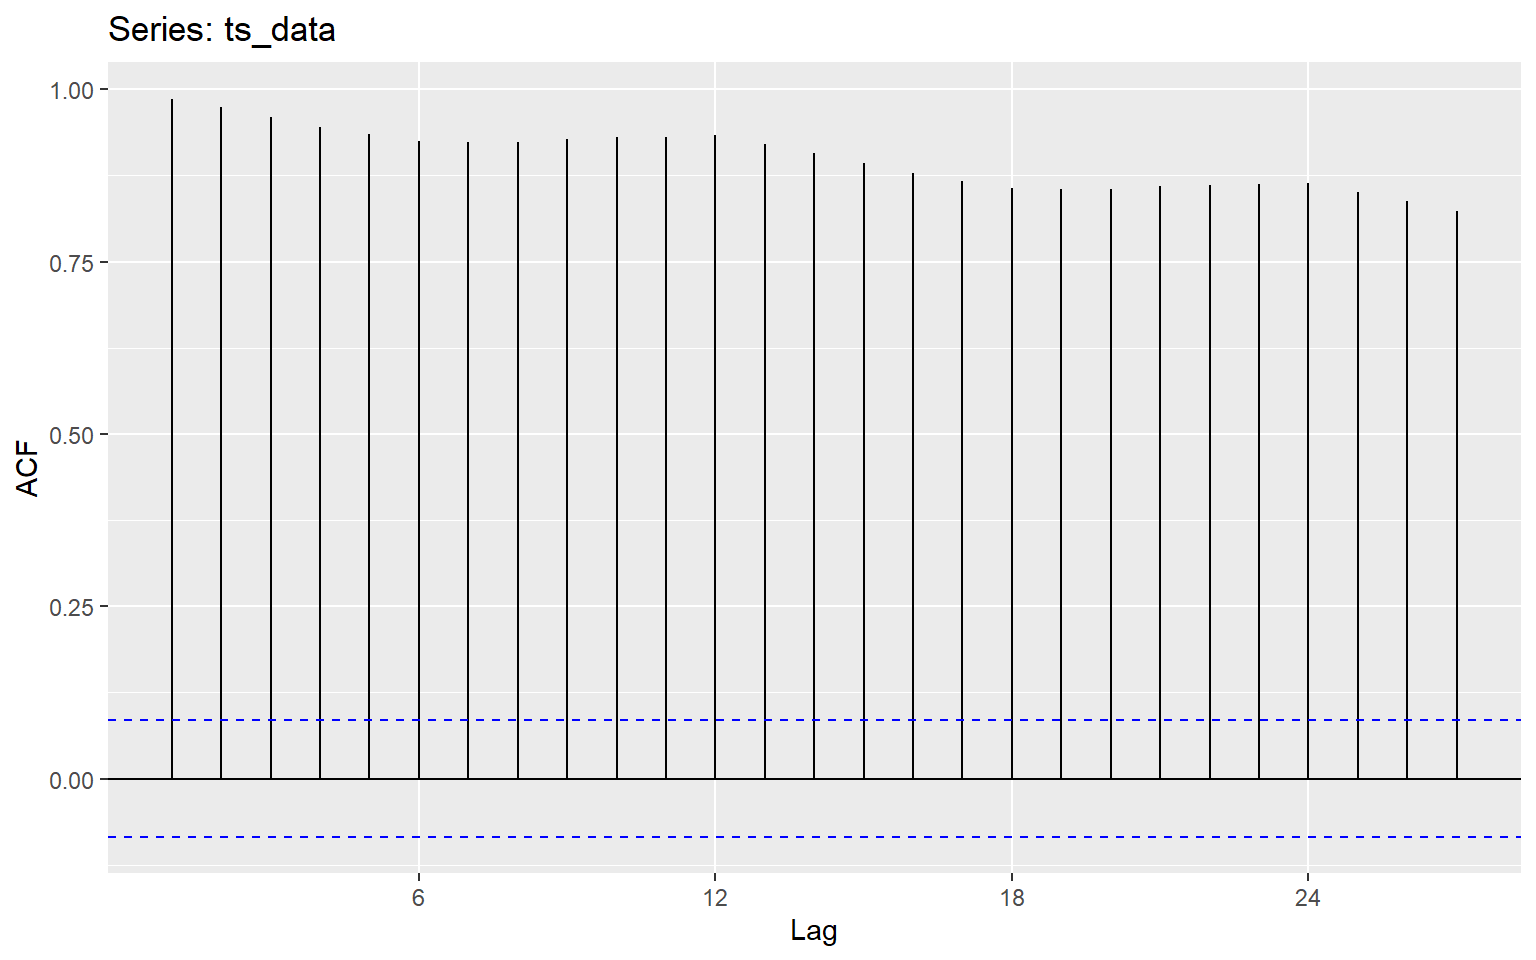
\includegraphics[keepaspectratio]{04-chap4_files/figure-pdf/unnamed-chunk-1-1.pdf}}

}

\caption{ACF and PACF of AR(1), MA(1) and ARMA(1, 1) models calculated
from the data}

\end{figure}%

\bookmarksetup{startatroot}

\chapter{References}\label{references}

Box, G. E., Jenkins, G. M., Reinsel, G. C., \& Ljung, G. M. (2015). Time
series analysis: forecasting and control.

\bookmarksetup{startatroot}

\chapter*{Bibliography}\label{bibliography}
\addcontentsline{toc}{chapter}{Bibliography}

\markboth{Bibliography}{Bibliography}

\printbibliography[heading=none]





\end{document}
